\documentclass[]{book}
\usepackage{lmodern}
\usepackage{amssymb,amsmath}
\usepackage{ifxetex,ifluatex}
\usepackage{fixltx2e} % provides \textsubscript
\ifnum 0\ifxetex 1\fi\ifluatex 1\fi=0 % if pdftex
  \usepackage[T1]{fontenc}
  \usepackage[utf8]{inputenc}
\else % if luatex or xelatex
  \ifxetex
    \usepackage{mathspec}
  \else
    \usepackage{fontspec}
  \fi
  \defaultfontfeatures{Ligatures=TeX,Scale=MatchLowercase}
\fi
% use upquote if available, for straight quotes in verbatim environments
\IfFileExists{upquote.sty}{\usepackage{upquote}}{}
% use microtype if available
\IfFileExists{microtype.sty}{%
\usepackage{microtype}
\UseMicrotypeSet[protrusion]{basicmath} % disable protrusion for tt fonts
}{}
\usepackage[margin=1in]{geometry}
\usepackage{hyperref}
\hypersetup{unicode=true,
            pdftitle={Feature Engineering},
            pdfauthor={Alfonso R. Reyes},
            pdfborder={0 0 0},
            breaklinks=true}
\urlstyle{same}  % don't use monospace font for urls
\usepackage{natbib}
\bibliographystyle{apalike}
\usepackage{color}
\usepackage{fancyvrb}
\newcommand{\VerbBar}{|}
\newcommand{\VERB}{\Verb[commandchars=\\\{\}]}
\DefineVerbatimEnvironment{Highlighting}{Verbatim}{commandchars=\\\{\}}
% Add ',fontsize=\small' for more characters per line
\usepackage{framed}
\definecolor{shadecolor}{RGB}{248,248,248}
\newenvironment{Shaded}{\begin{snugshade}}{\end{snugshade}}
\newcommand{\AlertTok}[1]{\textcolor[rgb]{0.94,0.16,0.16}{#1}}
\newcommand{\AnnotationTok}[1]{\textcolor[rgb]{0.56,0.35,0.01}{\textbf{\textit{#1}}}}
\newcommand{\AttributeTok}[1]{\textcolor[rgb]{0.77,0.63,0.00}{#1}}
\newcommand{\BaseNTok}[1]{\textcolor[rgb]{0.00,0.00,0.81}{#1}}
\newcommand{\BuiltInTok}[1]{#1}
\newcommand{\CharTok}[1]{\textcolor[rgb]{0.31,0.60,0.02}{#1}}
\newcommand{\CommentTok}[1]{\textcolor[rgb]{0.56,0.35,0.01}{\textit{#1}}}
\newcommand{\CommentVarTok}[1]{\textcolor[rgb]{0.56,0.35,0.01}{\textbf{\textit{#1}}}}
\newcommand{\ConstantTok}[1]{\textcolor[rgb]{0.00,0.00,0.00}{#1}}
\newcommand{\ControlFlowTok}[1]{\textcolor[rgb]{0.13,0.29,0.53}{\textbf{#1}}}
\newcommand{\DataTypeTok}[1]{\textcolor[rgb]{0.13,0.29,0.53}{#1}}
\newcommand{\DecValTok}[1]{\textcolor[rgb]{0.00,0.00,0.81}{#1}}
\newcommand{\DocumentationTok}[1]{\textcolor[rgb]{0.56,0.35,0.01}{\textbf{\textit{#1}}}}
\newcommand{\ErrorTok}[1]{\textcolor[rgb]{0.64,0.00,0.00}{\textbf{#1}}}
\newcommand{\ExtensionTok}[1]{#1}
\newcommand{\FloatTok}[1]{\textcolor[rgb]{0.00,0.00,0.81}{#1}}
\newcommand{\FunctionTok}[1]{\textcolor[rgb]{0.00,0.00,0.00}{#1}}
\newcommand{\ImportTok}[1]{#1}
\newcommand{\InformationTok}[1]{\textcolor[rgb]{0.56,0.35,0.01}{\textbf{\textit{#1}}}}
\newcommand{\KeywordTok}[1]{\textcolor[rgb]{0.13,0.29,0.53}{\textbf{#1}}}
\newcommand{\NormalTok}[1]{#1}
\newcommand{\OperatorTok}[1]{\textcolor[rgb]{0.81,0.36,0.00}{\textbf{#1}}}
\newcommand{\OtherTok}[1]{\textcolor[rgb]{0.56,0.35,0.01}{#1}}
\newcommand{\PreprocessorTok}[1]{\textcolor[rgb]{0.56,0.35,0.01}{\textit{#1}}}
\newcommand{\RegionMarkerTok}[1]{#1}
\newcommand{\SpecialCharTok}[1]{\textcolor[rgb]{0.00,0.00,0.00}{#1}}
\newcommand{\SpecialStringTok}[1]{\textcolor[rgb]{0.31,0.60,0.02}{#1}}
\newcommand{\StringTok}[1]{\textcolor[rgb]{0.31,0.60,0.02}{#1}}
\newcommand{\VariableTok}[1]{\textcolor[rgb]{0.00,0.00,0.00}{#1}}
\newcommand{\VerbatimStringTok}[1]{\textcolor[rgb]{0.31,0.60,0.02}{#1}}
\newcommand{\WarningTok}[1]{\textcolor[rgb]{0.56,0.35,0.01}{\textbf{\textit{#1}}}}
\usepackage{longtable,booktabs}
\usepackage{graphicx,grffile}
\makeatletter
\def\maxwidth{\ifdim\Gin@nat@width>\linewidth\linewidth\else\Gin@nat@width\fi}
\def\maxheight{\ifdim\Gin@nat@height>\textheight\textheight\else\Gin@nat@height\fi}
\makeatother
% Scale images if necessary, so that they will not overflow the page
% margins by default, and it is still possible to overwrite the defaults
% using explicit options in \includegraphics[width, height, ...]{}
\setkeys{Gin}{width=\maxwidth,height=\maxheight,keepaspectratio}
\IfFileExists{parskip.sty}{%
\usepackage{parskip}
}{% else
\setlength{\parindent}{0pt}
\setlength{\parskip}{6pt plus 2pt minus 1pt}
}
\setlength{\emergencystretch}{3em}  % prevent overfull lines
\providecommand{\tightlist}{%
  \setlength{\itemsep}{0pt}\setlength{\parskip}{0pt}}
\setcounter{secnumdepth}{5}
% Redefines (sub)paragraphs to behave more like sections
\ifx\paragraph\undefined\else
\let\oldparagraph\paragraph
\renewcommand{\paragraph}[1]{\oldparagraph{#1}\mbox{}}
\fi
\ifx\subparagraph\undefined\else
\let\oldsubparagraph\subparagraph
\renewcommand{\subparagraph}[1]{\oldsubparagraph{#1}\mbox{}}
\fi

%%% Use protect on footnotes to avoid problems with footnotes in titles
\let\rmarkdownfootnote\footnote%
\def\footnote{\protect\rmarkdownfootnote}

%%% Change title format to be more compact
\usepackage{titling}

% Create subtitle command for use in maketitle
\providecommand{\subtitle}[1]{
  \posttitle{
    \begin{center}\large#1\end{center}
    }
}

\setlength{\droptitle}{-2em}

  \title{Feature Engineering}
    \pretitle{\vspace{\droptitle}\centering\huge}
  \posttitle{\par}
    \author{Alfonso R. Reyes}
    \preauthor{\centering\large\emph}
  \postauthor{\par}
      \predate{\centering\large\emph}
  \postdate{\par}
    \date{2019-09-18}

\usepackage{booktabs}

\begin{document}
\maketitle

{
\setcounter{tocdepth}{1}
\tableofcontents
}
\hypertarget{prerequisites}{%
\chapter*{Prerequisites}\label{prerequisites}}
\addcontentsline{toc}{chapter}{Prerequisites}

\begin{Shaded}
\begin{Highlighting}[]
\KeywordTok{print}\NormalTok{(assets_dir)}
\CommentTok{#> [1] "/home/datascience/repos/machine-learning-rsuite/import/assets"}
\NormalTok{image_file <-}\StringTok{ }\KeywordTok{file.path}\NormalTok{(assets_dir, }\StringTok{"linear_regression.jpg"}\NormalTok{)}
\KeywordTok{file.exists}\NormalTok{(image_file)}
\CommentTok{#> [1] TRUE}
\end{Highlighting}
\end{Shaded}

\begin{Shaded}
\begin{Highlighting}[]
\NormalTok{knitr}\OperatorTok{::}\KeywordTok{include_graphics}\NormalTok{(image_file)}
\end{Highlighting}
\end{Shaded}

\begin{center}\includegraphics[width=0.7\linewidth]{/home/datascience/repos/machine-learning-rsuite/import/assets/linear_regression} \end{center}

This is a \emph{sample} book written in \textbf{Markdown}. You can use anything that Pandoc's Markdown supports, e.g., a math equation \(a^2 + b^2 = c^2\).

The \textbf{bookdown} package can be installed from CRAN or Github:

\begin{Shaded}
\begin{Highlighting}[]
\KeywordTok{install.packages}\NormalTok{(}\StringTok{"bookdown"}\NormalTok{)}
\CommentTok{# or the development version}
\CommentTok{# devtools::install_github("rstudio/bookdown")}
\end{Highlighting}
\end{Shaded}

Remember each Rmd file contains one and only one chapter, and a chapter is defined by the first-level heading \texttt{\#}.

To compile this example to PDF, you need XeLaTeX. You are recommended to install TinyTeX (which includes XeLaTeX): \url{https://yihui.name/tinytex/}.

\hypertarget{employee-attrition.-employee-attrition-dataset.-lime-package}{%
\chapter{\texorpdfstring{Employee attrition. Employee-Attrition dataset. \emph{LIME} package}{Employee attrition. Employee-Attrition dataset. LIME package}}\label{employee-attrition.-employee-attrition-dataset.-lime-package}}

Article: \url{https://www.business-science.io/business/2017/09/18/hr_employee_attrition.html}
Data: \url{https://www.ibm.com/communities/analytics/watson-analytics-blog/hr-employee-attrition/}

\hypertarget{introduction}{%
\section{Introduction}\label{introduction}}

\hypertarget{employee-attrition-a-major-problem}{%
\subsection{Employee attrition: a major problem}\label{employee-attrition-a-major-problem}}

Bill Gates was once quoted as saying,

\begin{quote}
``You take away our top 20 employees and we {[}Microsoft{]} become a mediocre company''.
\end{quote}

His statement cuts to the core of a major problem: employee attrition. An organization is only as good as its employees, and these people are the true source of its competitive advantage.

Organizations face huge costs resulting from employee turnover. Some costs are tangible such as training expenses and the time it takes from when an employee starts to when they become a productive member. However, the most important costs are intangible. Consider what's lost when a productive employee quits: new product ideas, great project management, or customer relationships.

With advances in machine learning and data science, its possible to not only predict employee attrition but to understand the key variables that influence turnover. We'll take a look at two cutting edge techniques:

\begin{enumerate}
\def\labelenumi{\arabic{enumi}.}
\item
  Machine Learning with \texttt{h2o.automl()} from the h2o package: This function takes automated machine learning to the next level by testing a number of advanced algorithms such as random forests, ensemble methods, and deep learning along with more traditional algorithms such as logistic regression. The main takeaway is that we can now easily achieve predictive performance that is in the same ball park (and in some cases even better than) commercial algorithms and ML/AI software.
\item
  Feature Importance with the \texttt{lime} package: The problem with advanced machine learning algorithms such as deep learning is that it's near impossible to understand the algorithm because of its complexity. This has all changed with the lime package. The major advancement with lime is that, by recursively analyzing the models locally, it can extract feature importance that repeats globally. What this means to us is that lime has opened the door to understanding the ML models regardless of complexity. Now the best (and typically very complex) models can also be investigated and potentially understood as to what variables or features make the model tick.
\end{enumerate}

\hypertarget{employee-attrition-machine-learning-analysis}{%
\subsection{Employee attrition: machine learning analysis}\label{employee-attrition-machine-learning-analysis}}

With these new automated ML tools combined with tools to uncover critical variables, we now have capabilities for both extreme predictive accuracy and understandability, which was previously impossible! We'll investigate an HR Analytic example of employee attrition that was evaluated by IBM Watson.

\hypertarget{where-we-got-the-data}{%
\subsection{Where we got the data}\label{where-we-got-the-data}}

The example comes from IBM Watson Analytics website. You can download the data and read the analysis here:

Get data used in this post here.
Read IBM Watson Analytics article here.
To summarize, the article makes a usage case for IBM Watson as an automated ML platform. The article shows that using Watson, the analyst was able to detect features that led to increased probability of attrition.

\hypertarget{automated-machine-learning-what-we-did-with-the-data}{%
\subsection{Automated machine learning (what we did with the data)}\label{automated-machine-learning-what-we-did-with-the-data}}

In this example we'll show how we can use the combination of H2O for developing a complex model with high predictive accuracy on unseen data and then how we can use LIME to understand important features related to employee attrition.

\hypertarget{load-packages}{%
\subsection{Load packages}\label{load-packages}}

Load the following packages.

\begin{Shaded}
\begin{Highlighting}[]
\CommentTok{# Load the following packages}
\KeywordTok{library}\NormalTok{(tidyquant)  }\CommentTok{# Loads tidyverse and several other pkgs }
\KeywordTok{library}\NormalTok{(readxl)     }\CommentTok{# Super simple excel reader}
\KeywordTok{library}\NormalTok{(h2o)        }\CommentTok{# Professional grade ML pkg}
\KeywordTok{library}\NormalTok{(lime)       }\CommentTok{# Explain complex black-box ML models}
\end{Highlighting}
\end{Shaded}

\hypertarget{load-data}{%
\subsection{Load data}\label{load-data}}

Download the data here. You can load the data using read\_excel(), pointing the path to your local file.

\begin{Shaded}
\begin{Highlighting}[]
\CommentTok{# Read excel data}
\NormalTok{hr_data_raw <-}\StringTok{ }\KeywordTok{read_excel}\NormalTok{(}\DataTypeTok{path =} \KeywordTok{file.path}\NormalTok{(data_raw_dir,}
                                           \StringTok{"WA_Fn-UseC_-HR-Employee-Attrition.xlsx"}\NormalTok{))}
\end{Highlighting}
\end{Shaded}

Let's check out the raw data. It's 1470 rows (observations) by 35 columns (features). The ``Attrition'' column is our target. We'll use all other columns as features to our model.

\begin{Shaded}
\begin{Highlighting}[]
\CommentTok{# View first 10 rows}
\NormalTok{hr_data_raw[}\DecValTok{1}\OperatorTok{:}\DecValTok{10}\NormalTok{,] }\OperatorTok
\StringTok{    }\NormalTok{knitr}\OperatorTok{::}\KeywordTok{kable}\NormalTok{(}\DataTypeTok{caption =} \StringTok{"First 10 rows"}\NormalTok{)}
\end{Highlighting}
\end{Shaded}

\begin{table}[t]

\caption{\label{tab:unnamed-chunk-2}First 10 rows}
\centering
\begin{tabular}{r|l|l|r|l|r|r|l|r|r|r|l|r|r|r|l|r|l|r|r|r|l|l|r|r|r|r|r|r|r|r|r|r|r|r}
\hline
Age & Attrition & BusinessTravel & DailyRate & Department & DistanceFromHome & Education & EducationField & EmployeeCount & EmployeeNumber & EnvironmentSatisfaction & Gender & HourlyRate & JobInvolvement & JobLevel & JobRole & JobSatisfaction & MaritalStatus & MonthlyIncome & MonthlyRate & NumCompaniesWorked & Over18 & OverTime & PercentSalaryHike & PerformanceRating & RelationshipSatisfaction & StandardHours & StockOptionLevel & TotalWorkingYears & TrainingTimesLastYear & WorkLifeBalance & YearsAtCompany & YearsInCurrentRole & YearsSinceLastPromotion & YearsWithCurrManager\\
\hline
41 & Yes & Travel\_Rarely & 1102 & Sales & 1 & 2 & Life Sciences & 1 & 1 & 2 & Female & 94 & 3 & 2 & Sales Executive & 4 & Single & 5993 & 19479 & 8 & Y & Yes & 11 & 3 & 1 & 80 & 0 & 8 & 0 & 1 & 6 & 4 & 0 & 5\\
\hline
49 & No & Travel\_Frequently & 279 & Research \& Development & 8 & 1 & Life Sciences & 1 & 2 & 3 & Male & 61 & 2 & 2 & Research Scientist & 2 & Married & 5130 & 24907 & 1 & Y & No & 23 & 4 & 4 & 80 & 1 & 10 & 3 & 3 & 10 & 7 & 1 & 7\\
\hline
37 & Yes & Travel\_Rarely & 1373 & Research \& Development & 2 & 2 & Other & 1 & 4 & 4 & Male & 92 & 2 & 1 & Laboratory Technician & 3 & Single & 2090 & 2396 & 6 & Y & Yes & 15 & 3 & 2 & 80 & 0 & 7 & 3 & 3 & 0 & 0 & 0 & 0\\
\hline
33 & No & Travel\_Frequently & 1392 & Research \& Development & 3 & 4 & Life Sciences & 1 & 5 & 4 & Female & 56 & 3 & 1 & Research Scientist & 3 & Married & 2909 & 23159 & 1 & Y & Yes & 11 & 3 & 3 & 80 & 0 & 8 & 3 & 3 & 8 & 7 & 3 & 0\\
\hline
27 & No & Travel\_Rarely & 591 & Research \& Development & 2 & 1 & Medical & 1 & 7 & 1 & Male & 40 & 3 & 1 & Laboratory Technician & 2 & Married & 3468 & 16632 & 9 & Y & No & 12 & 3 & 4 & 80 & 1 & 6 & 3 & 3 & 2 & 2 & 2 & 2\\
\hline
32 & No & Travel\_Frequently & 1005 & Research \& Development & 2 & 2 & Life Sciences & 1 & 8 & 4 & Male & 79 & 3 & 1 & Laboratory Technician & 4 & Single & 3068 & 11864 & 0 & Y & No & 13 & 3 & 3 & 80 & 0 & 8 & 2 & 2 & 7 & 7 & 3 & 6\\
\hline
59 & No & Travel\_Rarely & 1324 & Research \& Development & 3 & 3 & Medical & 1 & 10 & 3 & Female & 81 & 4 & 1 & Laboratory Technician & 1 & Married & 2670 & 9964 & 4 & Y & Yes & 20 & 4 & 1 & 80 & 3 & 12 & 3 & 2 & 1 & 0 & 0 & 0\\
\hline
30 & No & Travel\_Rarely & 1358 & Research \& Development & 24 & 1 & Life Sciences & 1 & 11 & 4 & Male & 67 & 3 & 1 & Laboratory Technician & 3 & Divorced & 2693 & 13335 & 1 & Y & No & 22 & 4 & 2 & 80 & 1 & 1 & 2 & 3 & 1 & 0 & 0 & 0\\
\hline
38 & No & Travel\_Frequently & 216 & Research \& Development & 23 & 3 & Life Sciences & 1 & 12 & 4 & Male & 44 & 2 & 3 & Manufacturing Director & 3 & Single & 9526 & 8787 & 0 & Y & No & 21 & 4 & 2 & 80 & 0 & 10 & 2 & 3 & 9 & 7 & 1 & 8\\
\hline
36 & No & Travel\_Rarely & 1299 & Research \& Development & 27 & 3 & Medical & 1 & 13 & 3 & Male & 94 & 3 & 2 & Healthcare Representative & 3 & Married & 5237 & 16577 & 6 & Y & No & 13 & 3 & 2 & 80 & 2 & 17 & 3 & 2 & 7 & 7 & 7 & 7\\
\hline
\end{tabular}
\end{table}

The only pre-processing we'll do in this example is change all character data types to factors. This is needed for H2O. We could make a number of other numeric data that is actually categorical factors, but this tends to increase modeling time and can have little improvement on model performance.

\begin{Shaded}
\begin{Highlighting}[]
\NormalTok{hr_data <-}\StringTok{ }\NormalTok{hr_data_raw }\OperatorTok
\StringTok{    }\KeywordTok{mutate_if}\NormalTok{(is.character, as.factor) }\OperatorTok
\StringTok{    }\KeywordTok{select}\NormalTok{(Attrition, }\KeywordTok{everything}\NormalTok{())}
\end{Highlighting}
\end{Shaded}

Let's take a glimpse at the processed dataset. We can see all of the columns. Note our target (``Attrition'') is the first column.

\begin{Shaded}
\begin{Highlighting}[]
\KeywordTok{glimpse}\NormalTok{(hr_data)}
\CommentTok{#> Observations: 1,470}
\CommentTok{#> Variables: 35}
\CommentTok{#> $ Attrition                <fct> Yes, No, Yes, No, No, No, No, No, No,...}
\CommentTok{#> $ Age                      <dbl> 41, 49, 37, 33, 27, 32, 59, 30, 38, 3...}
\CommentTok{#> $ BusinessTravel           <fct> Travel_Rarely, Travel_Frequently, Tra...}
\CommentTok{#> $ DailyRate                <dbl> 1102, 279, 1373, 1392, 591, 1005, 132...}
\CommentTok{#> $ Department               <fct> Sales, Research & Development, Resear...}
\CommentTok{#> $ DistanceFromHome         <dbl> 1, 8, 2, 3, 2, 2, 3, 24, 23, 27, 16, ...}
\CommentTok{#> $ Education                <dbl> 2, 1, 2, 4, 1, 2, 3, 1, 3, 3, 3, 2, 1...}
\CommentTok{#> $ EducationField           <fct> Life Sciences, Life Sciences, Other, ...}
\CommentTok{#> $ EmployeeCount            <dbl> 1, 1, 1, 1, 1, 1, 1, 1, 1, 1, 1, 1, 1...}
\CommentTok{#> $ EmployeeNumber           <dbl> 1, 2, 4, 5, 7, 8, 10, 11, 12, 13, 14,...}
\CommentTok{#> $ EnvironmentSatisfaction  <dbl> 2, 3, 4, 4, 1, 4, 3, 4, 4, 3, 1, 4, 1...}
\CommentTok{#> $ Gender                   <fct> Female, Male, Male, Female, Male, Mal...}
\CommentTok{#> $ HourlyRate               <dbl> 94, 61, 92, 56, 40, 79, 81, 67, 44, 9...}
\CommentTok{#> $ JobInvolvement           <dbl> 3, 2, 2, 3, 3, 3, 4, 3, 2, 3, 4, 2, 3...}
\CommentTok{#> $ JobLevel                 <dbl> 2, 2, 1, 1, 1, 1, 1, 1, 3, 2, 1, 2, 1...}
\CommentTok{#> $ JobRole                  <fct> Sales Executive, Research Scientist, ...}
\CommentTok{#> $ JobSatisfaction          <dbl> 4, 2, 3, 3, 2, 4, 1, 3, 3, 3, 2, 3, 3...}
\CommentTok{#> $ MaritalStatus            <fct> Single, Married, Single, Married, Mar...}
\CommentTok{#> $ MonthlyIncome            <dbl> 5993, 5130, 2090, 2909, 3468, 3068, 2...}
\CommentTok{#> $ MonthlyRate              <dbl> 19479, 24907, 2396, 23159, 16632, 118...}
\CommentTok{#> $ NumCompaniesWorked       <dbl> 8, 1, 6, 1, 9, 0, 4, 1, 0, 6, 0, 0, 1...}
\CommentTok{#> $ Over18                   <fct> Y, Y, Y, Y, Y, Y, Y, Y, Y, Y, Y, Y, Y...}
\CommentTok{#> $ OverTime                 <fct> Yes, No, Yes, Yes, No, No, Yes, No, N...}
\CommentTok{#> $ PercentSalaryHike        <dbl> 11, 23, 15, 11, 12, 13, 20, 22, 21, 1...}
\CommentTok{#> $ PerformanceRating        <dbl> 3, 4, 3, 3, 3, 3, 4, 4, 4, 3, 3, 3, 3...}
\CommentTok{#> $ RelationshipSatisfaction <dbl> 1, 4, 2, 3, 4, 3, 1, 2, 2, 2, 3, 4, 4...}
\CommentTok{#> $ StandardHours            <dbl> 80, 80, 80, 80, 80, 80, 80, 80, 80, 8...}
\CommentTok{#> $ StockOptionLevel         <dbl> 0, 1, 0, 0, 1, 0, 3, 1, 0, 2, 1, 0, 1...}
\CommentTok{#> $ TotalWorkingYears        <dbl> 8, 10, 7, 8, 6, 8, 12, 1, 10, 17, 6, ...}
\CommentTok{#> $ TrainingTimesLastYear    <dbl> 0, 3, 3, 3, 3, 2, 3, 2, 2, 3, 5, 3, 1...}
\CommentTok{#> $ WorkLifeBalance          <dbl> 1, 3, 3, 3, 3, 2, 2, 3, 3, 2, 3, 3, 2...}
\CommentTok{#> $ YearsAtCompany           <dbl> 6, 10, 0, 8, 2, 7, 1, 1, 9, 7, 5, 9, ...}
\CommentTok{#> $ YearsInCurrentRole       <dbl> 4, 7, 0, 7, 2, 7, 0, 0, 7, 7, 4, 5, 2...}
\CommentTok{#> $ YearsSinceLastPromotion  <dbl> 0, 1, 0, 3, 2, 3, 0, 0, 1, 7, 0, 0, 4...}
\CommentTok{#> $ YearsWithCurrManager     <dbl> 5, 7, 0, 0, 2, 6, 0, 0, 8, 7, 3, 8, 3...}
\end{Highlighting}
\end{Shaded}

\hypertarget{modeling-employee-attrition}{%
\section{Modeling Employee attrition}\label{modeling-employee-attrition}}

We are going to use the \texttt{h2o.automl()} function from the H2O platform to model employee attrition.

\hypertarget{machine-learning-with-h2o}{%
\subsection{\texorpdfstring{Machine Learning with \texttt{h2o}}{Machine Learning with h2o}}\label{machine-learning-with-h2o}}

First, we need to initialize the \emph{Java Virtual Machine (JVM)} that H2O uses locally.

\begin{Shaded}
\begin{Highlighting}[]
\CommentTok{# Initialize H2O JVM}
\KeywordTok{h2o.init}\NormalTok{()}
\CommentTok{#> }
\CommentTok{#> H2O is not running yet, starting it now...}
\CommentTok{#> }
\CommentTok{#> Note:  In case of errors look at the following log files:}
\CommentTok{#>     /tmp/RtmpCSPWrv/h2o_datascience_started_from_r.out}
\CommentTok{#>     /tmp/RtmpCSPWrv/h2o_datascience_started_from_r.err}
\CommentTok{#> }
\CommentTok{#> }
\CommentTok{#> Starting H2O JVM and connecting: . Connection successful!}
\CommentTok{#> }
\CommentTok{#> R is connected to the H2O cluster: }
\CommentTok{#>     H2O cluster uptime:         1 seconds 256 milliseconds }
\CommentTok{#>     H2O cluster timezone:       America/Chicago }
\CommentTok{#>     H2O data parsing timezone:  UTC }
\CommentTok{#>     H2O cluster version:        3.22.1.1 }
\CommentTok{#>     H2O cluster version age:    8 months and 20 days !!! }
\CommentTok{#>     H2O cluster name:           H2O_started_from_R_datascience_mwl453 }
\CommentTok{#>     H2O cluster total nodes:    1 }
\CommentTok{#>     H2O cluster total memory:   6.96 GB }
\CommentTok{#>     H2O cluster total cores:    8 }
\CommentTok{#>     H2O cluster allowed cores:  8 }
\CommentTok{#>     H2O cluster healthy:        TRUE }
\CommentTok{#>     H2O Connection ip:          localhost }
\CommentTok{#>     H2O Connection port:        54321 }
\CommentTok{#>     H2O Connection proxy:       NA }
\CommentTok{#>     H2O Internal Security:      FALSE }
\CommentTok{#>     H2O API Extensions:         XGBoost, Algos, AutoML, Core V3, Core V4 }
\CommentTok{#>     R Version:                  R version 3.6.0 (2019-04-26)}
\KeywordTok{h2o.no_progress}\NormalTok{() }\CommentTok{# Turn off output of progress bars}
\end{Highlighting}
\end{Shaded}

Next, we change our data to an h2o object that the package can interpret. We also split the data into training, validation, and test sets. Our preference is to use 70\%, 15\%, 15\%, respectively.

\begin{Shaded}
\begin{Highlighting}[]
\CommentTok{# Split data into Train/Validation/Test Sets}
\NormalTok{hr_data_h2o <-}\StringTok{ }\KeywordTok{as.h2o}\NormalTok{(hr_data)}

\NormalTok{split_h2o <-}\StringTok{ }\KeywordTok{h2o.splitFrame}\NormalTok{(hr_data_h2o, }\KeywordTok{c}\NormalTok{(}\FloatTok{0.7}\NormalTok{, }\FloatTok{0.15}\NormalTok{), }\DataTypeTok{seed =} \DecValTok{1234}\NormalTok{ )}
\NormalTok{train_h2o <-}\StringTok{ }\KeywordTok{h2o.assign}\NormalTok{(split_h2o[[}\DecValTok{1}\NormalTok{]], }\StringTok{"train"}\NormalTok{ ) }\CommentTok{# 70%}
\NormalTok{valid_h2o <-}\StringTok{ }\KeywordTok{h2o.assign}\NormalTok{(split_h2o[[}\DecValTok{2}\NormalTok{]], }\StringTok{"valid"}\NormalTok{ ) }\CommentTok{# 15%}
\NormalTok{test_h2o  <-}\StringTok{ }\KeywordTok{h2o.assign}\NormalTok{(split_h2o[[}\DecValTok{3}\NormalTok{]], }\StringTok{"test"}\NormalTok{ )  }\CommentTok{# 15%}
\end{Highlighting}
\end{Shaded}

\hypertarget{model}{%
\section{Model}\label{model}}

Now we are ready to model. We'll set the target and feature names. The target is what we aim to predict (in our case ``Attrition''). The features (every other column) are what we will use to model the prediction.

\begin{Shaded}
\begin{Highlighting}[]
\CommentTok{# Set names for h2o}
\NormalTok{y <-}\StringTok{ "Attrition"}
\NormalTok{x <-}\StringTok{ }\KeywordTok{setdiff}\NormalTok{(}\KeywordTok{names}\NormalTok{(train_h2o), y)}
\end{Highlighting}
\end{Shaded}

Now the fun begins. We run the h2o.automl() setting the arguments it needs to run models against. For more information, see the h2o.automl documentation.

\begin{itemize}
\tightlist
\item
  \texttt{x\ =\ x}: The names of our feature columns.
\item
  \texttt{y\ =\ y}: The name of our target column.
\item
  \texttt{training\_frame} = train\_h2o: Our training set consisting of 70\% of the data.
\item
  \texttt{leaderboard\_frame} = valid\_h2o: Our validation set consisting of 15\% of the data. H2O uses this to ensure the model does not overfit the data.
\item
  \texttt{max\_runtime\_secs\ =\ 30}: We supply this to speed up H2O's modeling. The algorithm has a large number of complex models so we want to keep things moving at the expense of some accuracy.
\end{itemize}

\begin{Shaded}
\begin{Highlighting}[]
\CommentTok{# Run the automated machine learning }
\NormalTok{automl_models_h2o <-}\StringTok{ }\KeywordTok{h2o.automl}\NormalTok{(}
    \DataTypeTok{x =}\NormalTok{ x, }
    \DataTypeTok{y =}\NormalTok{ y,}
    \DataTypeTok{training_frame    =}\NormalTok{ train_h2o,}
    \DataTypeTok{leaderboard_frame =}\NormalTok{ valid_h2o,}
    \DataTypeTok{max_runtime_secs  =} \DecValTok{30}
\NormalTok{    )}
\end{Highlighting}
\end{Shaded}

All of the models are stored the \texttt{automl\_models\_h2o} object. However, we are only concerned with the leader, which is the best model in terms of accuracy on the validation set. We'll extract it from the models object.

\begin{Shaded}
\begin{Highlighting}[]
\CommentTok{# Extract leader model}
\NormalTok{automl_leader <-}\StringTok{ }\NormalTok{automl_models_h2o}\OperatorTok{@}\NormalTok{leader}
\end{Highlighting}
\end{Shaded}

\hypertarget{predict}{%
\section{Predict}\label{predict}}

Now we are ready to predict on our test set, which is unseen from during our modeling process. This is the true test of performance. We use the \texttt{h2o.predict()} function to make predictions.\\

\begin{Shaded}
\begin{Highlighting}[]
\CommentTok{# Predict on hold-out set, test_h2o}
\NormalTok{pred_h2o <-}\StringTok{ }\KeywordTok{h2o.predict}\NormalTok{(}\DataTypeTok{object =}\NormalTok{ automl_leader, }\DataTypeTok{newdata =}\NormalTok{ test_h2o)}
\end{Highlighting}
\end{Shaded}

\hypertarget{performance}{%
\section{Performance}\label{performance}}

Now we can evaluate our leader model. We'll reformat the test set an add the predictions as column so we have the actual and prediction columns side-by-side.\\

\begin{Shaded}
\begin{Highlighting}[]
\CommentTok{# Prep for performance assessment}
\NormalTok{test_performance <-}\StringTok{ }\NormalTok{test_h2o }\OperatorTok
\StringTok{    }\NormalTok{tibble}\OperatorTok{::}\KeywordTok{as_tibble}\NormalTok{() }\OperatorTok
\StringTok{    }\KeywordTok{select}\NormalTok{(Attrition) }\OperatorTok
\StringTok{    }\KeywordTok{add_column}\NormalTok{(}\DataTypeTok{pred =} \KeywordTok{as.vector}\NormalTok{(pred_h2o}\OperatorTok{$}\NormalTok{predict)) }\OperatorTok
\StringTok{    }\KeywordTok{mutate_if}\NormalTok{(is.character, as.factor)}
\NormalTok{test_performance}
\CommentTok{#> # A tibble: 211 x 2}
\CommentTok{#>   Attrition pred }
\CommentTok{#>   <fct>     <fct>}
\CommentTok{#> 1 No        No   }
\CommentTok{#> 2 No        No   }
\CommentTok{#> 3 Yes       Yes  }
\CommentTok{#> 4 No        No   }
\CommentTok{#> 5 No        No   }
\CommentTok{#> 6 No        No   }
\CommentTok{#> # ... with 205 more rows}
\end{Highlighting}
\end{Shaded}

We can use the table() function to quickly get a confusion table of the results. We see that the leader model wasn't perfect, but it did a decent job identifying employees that are likely to quit. For perspective, a logistic regression would not perform nearly this well.\\

\begin{Shaded}
\begin{Highlighting}[]
\CommentTok{# Confusion table counts}
\NormalTok{confusion_matrix <-}\StringTok{ }\NormalTok{test_performance }\OperatorTok
\StringTok{    }\KeywordTok{table}\NormalTok{() }
\NormalTok{confusion_matrix}
\CommentTok{#>          pred}
\CommentTok{#> Attrition  No Yes}
\CommentTok{#>       No  165  17}
\CommentTok{#>       Yes   9  20}
\end{Highlighting}
\end{Shaded}

We'll run through a binary classification analysis to understand the model performance.

\begin{Shaded}
\begin{Highlighting}[]
\CommentTok{# Performance analysis}
\NormalTok{tn <-}\StringTok{ }\NormalTok{confusion_matrix[}\DecValTok{1}\NormalTok{]}
\NormalTok{tp <-}\StringTok{ }\NormalTok{confusion_matrix[}\DecValTok{4}\NormalTok{]}
\NormalTok{fp <-}\StringTok{ }\NormalTok{confusion_matrix[}\DecValTok{3}\NormalTok{]}
\NormalTok{fn <-}\StringTok{ }\NormalTok{confusion_matrix[}\DecValTok{2}\NormalTok{]}

\NormalTok{accuracy <-}\StringTok{ }\NormalTok{(tp }\OperatorTok{+}\StringTok{ }\NormalTok{tn) }\OperatorTok{/}\StringTok{ }\NormalTok{(tp }\OperatorTok{+}\StringTok{ }\NormalTok{tn }\OperatorTok{+}\StringTok{ }\NormalTok{fp }\OperatorTok{+}\StringTok{ }\NormalTok{fn)}
\NormalTok{misclassification_rate <-}\StringTok{ }\DecValTok{1} \OperatorTok{-}\StringTok{ }\NormalTok{accuracy}
\NormalTok{recall <-}\StringTok{ }\NormalTok{tp }\OperatorTok{/}\StringTok{ }\NormalTok{(tp }\OperatorTok{+}\StringTok{ }\NormalTok{fn)}
\NormalTok{precision <-}\StringTok{ }\NormalTok{tp }\OperatorTok{/}\StringTok{ }\NormalTok{(tp }\OperatorTok{+}\StringTok{ }\NormalTok{fp)}
\NormalTok{null_error_rate <-}\StringTok{ }\NormalTok{tn }\OperatorTok{/}\StringTok{ }\NormalTok{(tp }\OperatorTok{+}\StringTok{ }\NormalTok{tn }\OperatorTok{+}\StringTok{ }\NormalTok{fp }\OperatorTok{+}\StringTok{ }\NormalTok{fn)}

\KeywordTok{tibble}\NormalTok{(}
\NormalTok{    accuracy,}
\NormalTok{    misclassification_rate,}
\NormalTok{    recall,}
\NormalTok{    precision,}
\NormalTok{    null_error_rate}
\NormalTok{) }\OperatorTok\StringTok{ }
\StringTok{    }\KeywordTok{transpose}\NormalTok{() }
\CommentTok{#> [[1]]}
\CommentTok{#> [[1]]$accuracy}
\CommentTok{#> [1] 0.877}
\CommentTok{#> }
\CommentTok{#> [[1]]$misclassification_rate}
\CommentTok{#> [1] 0.123}
\CommentTok{#> }
\CommentTok{#> [[1]]$recall}
\CommentTok{#> [1] 0.69}
\CommentTok{#> }
\CommentTok{#> [[1]]$precision}
\CommentTok{#> [1] 0.541}
\CommentTok{#> }
\CommentTok{#> [[1]]$null_error_rate}
\CommentTok{#> [1] 0.782}
\end{Highlighting}
\end{Shaded}

It is important to understand is that the accuracy can be misleading: 88\% sounds pretty good especially for modeling HR data, but if we just pick \texttt{Attrition\ =\ NO} we would get an accuracy of about 79\%. Doesn't sound so great now.

Before we make our final judgement, let's dive a little deeper into precision and recall. Precision is when the model predicts yes, how often is it actually yes. Recall (also true positive rate or specificity) is when the actual value is yes how often is the model correct. Confused yet? Let's explain in terms of what's important to HR.

Most HR groups would probably prefer to incorrectly classify folks not looking to quit as high potential of quiting rather than classify those that are likely to quit as not at risk. Because it's important to not miss at risk employees, HR will really care about recall or when the actual value is \texttt{Attrition\ =\ YES} how often the model predicts YES.

Recall for our model is 62\%. In an HR context, this is 62\% more employees that could potentially be targeted prior to quiting. From that standpoint, an organization that loses 100 people per year could possibly target 62 implementing measures to retain.

\hypertarget{the-lime-package}{%
\section{\texorpdfstring{The \texttt{lime} package}{The lime package}}\label{the-lime-package}}

We have a very good model that is capable of making very accurate predictions on unseen data, but what can it tell us about what causes attrition? Let's find out using LIME.

\hypertarget{set-up}{%
\subsection{Set up}\label{set-up}}

The \texttt{lime} package implements LIME in R. One thing to note is that it's not setup out-of-the-box to work with \texttt{h2o}. The good news is with a few functions we can get everything working properly. We'll need to make two custom functions:

\begin{itemize}
\item
  \texttt{model\_type}: Used to tell lime what type of model we are dealing with. It could be classification, regression, survival, etc.
\item
  \texttt{predict\_model}: Used to allow lime to perform predictions that its algorithm can interpret.
\end{itemize}

The first thing we need to do is identify the class of our model leader object. We do this with the \texttt{class()} function.

\begin{Shaded}
\begin{Highlighting}[]
\KeywordTok{class}\NormalTok{(automl_leader)}
\CommentTok{#> [1] "H2OBinomialModel"}
\CommentTok{#> attr(,"package")}
\CommentTok{#> [1] "h2o"}
\end{Highlighting}
\end{Shaded}

Next we create our \texttt{model\_type} function. It's only input is x the h2o model. The function simply returns ``classification'', which tells LIME we are classifying.\\

\begin{Shaded}
\begin{Highlighting}[]
\CommentTok{# Setup lime::model_type() function for h2o}
\NormalTok{model_type.H2OBinomialModel <-}\StringTok{ }\ControlFlowTok{function}\NormalTok{(x, ...) \{}
    \CommentTok{# Function tells lime() what model type we are dealing with}
    \CommentTok{# 'classification', 'regression', 'survival', 'clustering', 'multilabel', etc}
    \CommentTok{#}
    \CommentTok{# x is our h2o model}
    
    \KeywordTok{return}\NormalTok{(}\StringTok{"classification"}\NormalTok{)}
\NormalTok{\}}
\end{Highlighting}
\end{Shaded}

Now we can create our \texttt{predict\_model} function. The trick here is to realize that it's inputs must be x a model, newdata a dataframe object (this is important), and type which is not used but can be use to switch the output type. The output is also a little tricky because it must be in the format of probabilities by classification (this is important; shown next). Internally we just call the \texttt{h2o.predict()} function.

\begin{Shaded}
\begin{Highlighting}[]
\CommentTok{# Setup lime::predict_model() function for h2o}
\NormalTok{predict_model.H2OBinomialModel <-}\StringTok{ }\ControlFlowTok{function}\NormalTok{(x, newdata, type, ...) \{}
    \CommentTok{# Function performs prediction and returns dataframe with Response}
    \CommentTok{#}
    \CommentTok{# x is h2o model}
    \CommentTok{# newdata is data frame}
    \CommentTok{# type is only setup for data frame}
    
\NormalTok{    pred <-}\StringTok{ }\KeywordTok{h2o.predict}\NormalTok{(x, }\KeywordTok{as.h2o}\NormalTok{(newdata))}
    
    \CommentTok{# return probs}
    \KeywordTok{return}\NormalTok{(}\KeywordTok{as.data.frame}\NormalTok{(pred[,}\OperatorTok{-}\DecValTok{1}\NormalTok{]))}
    
\NormalTok{\}}
\end{Highlighting}
\end{Shaded}

Run this next script to show you what the output looks like and to test our \texttt{predict\_model} function. See how it's the probabilities by classification. It must be in this form for \texttt{model\_type\ =\ “classification”}.

\begin{Shaded}
\begin{Highlighting}[]
\CommentTok{# Test our predict_model() function}
\KeywordTok{predict_model}\NormalTok{(}\DataTypeTok{x =}\NormalTok{ automl_leader, }\DataTypeTok{newdata =} \KeywordTok{as.data.frame}\NormalTok{(test_h2o[,}\OperatorTok{-}\DecValTok{1}\NormalTok{]), }\DataTypeTok{type =} \StringTok{'raw'}\NormalTok{) }\OperatorTok
\StringTok{    }\NormalTok{tibble}\OperatorTok{::}\KeywordTok{as_tibble}\NormalTok{()}
\CommentTok{#> # A tibble: 211 x 2}
\CommentTok{#>      No     Yes}
\CommentTok{#>   <dbl>   <dbl>}
\CommentTok{#> 1 0.812 0.188  }
\CommentTok{#> 2 0.940 0.0604 }
\CommentTok{#> 3 0.164 0.836  }
\CommentTok{#> 4 0.985 0.0152 }
\CommentTok{#> 5 0.808 0.192  }
\CommentTok{#> 6 0.991 0.00903}
\CommentTok{#> # ... with 205 more rows}
\end{Highlighting}
\end{Shaded}

Now the fun part, we create an explainer using the \texttt{lime()} function. Just pass the training data set without the ``Attribution column''. The form must be a data frame, which is OK since our predict\_model function will switch it to an h2o object. Set\texttt{model\ =\ automl\_leader} our leader model, and \texttt{bin\_continuous\ =\ FALSE}. We could tell the algorithm to bin continuous variables, but this may not make sense for categorical numeric data that we didn't change to factors.\\

\begin{Shaded}
\begin{Highlighting}[]
\CommentTok{# Run lime() on training set}
\NormalTok{explainer <-}\StringTok{ }\NormalTok{lime}\OperatorTok{::}\KeywordTok{lime}\NormalTok{(}
    \KeywordTok{as.data.frame}\NormalTok{(train_h2o[,}\OperatorTok{-}\DecValTok{1}\NormalTok{]), }
    \DataTypeTok{model          =}\NormalTok{ automl_leader, }
    \DataTypeTok{bin_continuous =} \OtherTok{FALSE}\NormalTok{)}
\CommentTok{#> Warning: Data contains numeric columns with zero variance}
\end{Highlighting}
\end{Shaded}

Now we run the \texttt{explain()} function, which returns our explanation. This can take a minute to run so we limit it to just the first ten rows of the test data set. We set n\_labels = 1 because we care about explaining a single class. Setting n\_features = 4 returns the top four features that are critical to each case. Finally, setting kernel\_width = 0.5 allows us to increase the ``model\_r2'' value by shrinking the localized evaluation.\\

\begin{Shaded}
\begin{Highlighting}[]
\CommentTok{# Run explain() on explainer}
\NormalTok{explanation <-}\StringTok{ }\NormalTok{lime}\OperatorTok{::}\KeywordTok{explain}\NormalTok{(}
    \KeywordTok{as.data.frame}\NormalTok{(test_h2o[}\DecValTok{1}\OperatorTok{:}\DecValTok{10}\NormalTok{,}\OperatorTok{-}\DecValTok{1}\NormalTok{]), }
    \DataTypeTok{explainer    =}\NormalTok{ explainer, }
    \DataTypeTok{n_labels     =} \DecValTok{1}\NormalTok{, }
    \DataTypeTok{n_features   =} \DecValTok{4}\NormalTok{,}
    \DataTypeTok{kernel_width =} \FloatTok{0.5}\NormalTok{)}
\end{Highlighting}
\end{Shaded}

\hypertarget{feature-importance-visualization}{%
\section{Feature Importance Visualization}\label{feature-importance-visualization}}

The payoff for the work we put in using LIME is this feature importance plot. This allows us to visualize each of the ten cases (observations) from the test data. The top four features for each case are shown. Note that they are not the same for each case. The green bars mean that the feature supports the model conclusion, and the red bars contradict. We'll focus in on Cases with \texttt{Label\ =\ Yes}, which are predicted to have attrition. We can see a common theme with Case 3 and Case 7: Training Time, Job Role, and Over Time are among the top factors influencing attrition. These are only two cases, but they can be used to potentially generalize to the larger population as we will see next.

\begin{Shaded}
\begin{Highlighting}[]
\KeywordTok{plot_features}\NormalTok{(explanation) }\OperatorTok{+}
\StringTok{    }\KeywordTok{labs}\NormalTok{(}\DataTypeTok{title =} \StringTok{"HR Predictive Analytics: LIME Feature Importance Visualization"}\NormalTok{,}
         \DataTypeTok{subtitle =} \StringTok{"Hold Out (Test) Set, First 10 Cases Shown"}\NormalTok{)}
\end{Highlighting}
\end{Shaded}

\begin{center}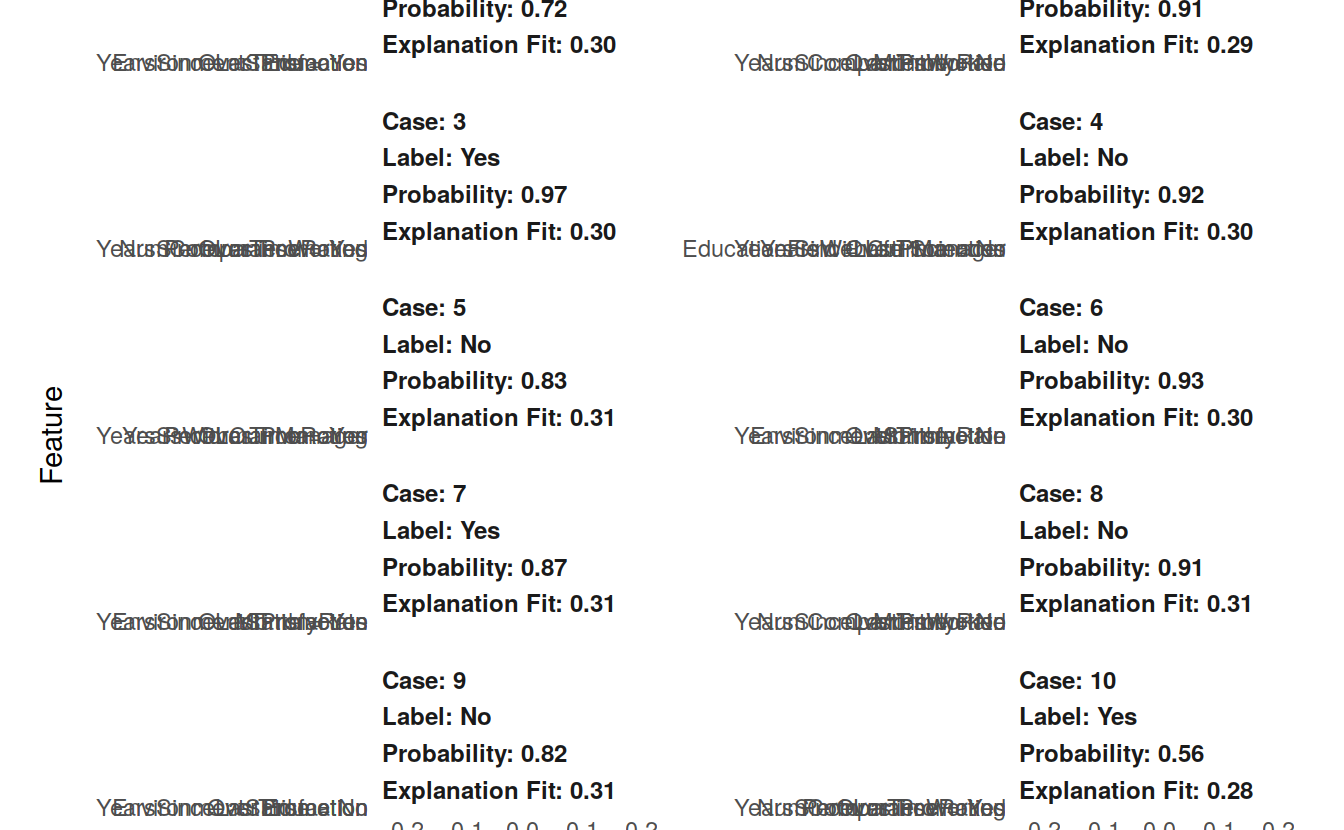
\includegraphics[width=0.7\linewidth]{comparison_342-classification_employee_attrition-lime-multi_files/figure-latex/plot-features-1} \end{center}

\hypertarget{what-features-are-linked-to-employee-attrition}{%
\subsection{What features are linked to employee attrition}\label{what-features-are-linked-to-employee-attrition}}

Now we turn to our three critical features from the LIME Feature Importance Plot:

\begin{itemize}
\tightlist
\item
  Training Time
\item
  Job Role
\item
  Over Time
\end{itemize}

We'll subset this data and visualize to detect trends.

\begin{Shaded}
\begin{Highlighting}[]
\CommentTok{# Focus on critical features of attrition}
\NormalTok{attrition_critical_features <-}\StringTok{ }\NormalTok{hr_data }\OperatorTok
\StringTok{    }\NormalTok{tibble}\OperatorTok{::}\KeywordTok{as_tibble}\NormalTok{() }\OperatorTok
\StringTok{    }\KeywordTok{select}\NormalTok{(Attrition, TrainingTimesLastYear, JobRole, OverTime) }\OperatorTok
\StringTok{    }\KeywordTok{rowid_to_column}\NormalTok{(}\DataTypeTok{var =} \StringTok{"Case"}\NormalTok{)}
\NormalTok{attrition_critical_features}
\CommentTok{#> # A tibble: 1,470 x 5}
\CommentTok{#>    Case Attrition TrainingTimesLastYear JobRole               OverTime}
\CommentTok{#>   <int> <fct>                     <dbl> <fct>                 <fct>   }
\CommentTok{#> 1     1 Yes                           0 Sales Executive       Yes     }
\CommentTok{#> 2     2 No                            3 Research Scientist    No      }
\CommentTok{#> 3     3 Yes                           3 Laboratory Technician Yes     }
\CommentTok{#> 4     4 No                            3 Research Scientist    Yes     }
\CommentTok{#> 5     5 No                            3 Laboratory Technician No      }
\CommentTok{#> 6     6 No                            2 Laboratory Technician No      }
\CommentTok{#> # ... with 1,464 more rows}
\end{Highlighting}
\end{Shaded}

\hypertarget{training}{%
\subsection{Training}\label{training}}

From the violin plot, the employees that stay tend to have a large peaks at two and three trainings per year whereas the employees that leave tend to have a large peak at two trainings per year. This suggests that employees with more trainings may be less likely to leave.\\

\begin{Shaded}
\begin{Highlighting}[]
\KeywordTok{ggplot}\NormalTok{(attrition_critical_features, }\KeywordTok{aes}\NormalTok{(}\DataTypeTok{x =}\NormalTok{ Attrition, }
                                        \DataTypeTok{y =}\NormalTok{ TrainingTimesLastYear)) }\OperatorTok{+}
\StringTok{    }\KeywordTok{geom_violin}\NormalTok{()  }\OperatorTok{+}
\StringTok{    }\KeywordTok{geom_jitter}\NormalTok{(}\DataTypeTok{alpha =} \FloatTok{0.25}\NormalTok{)}
\end{Highlighting}
\end{Shaded}

\begin{center}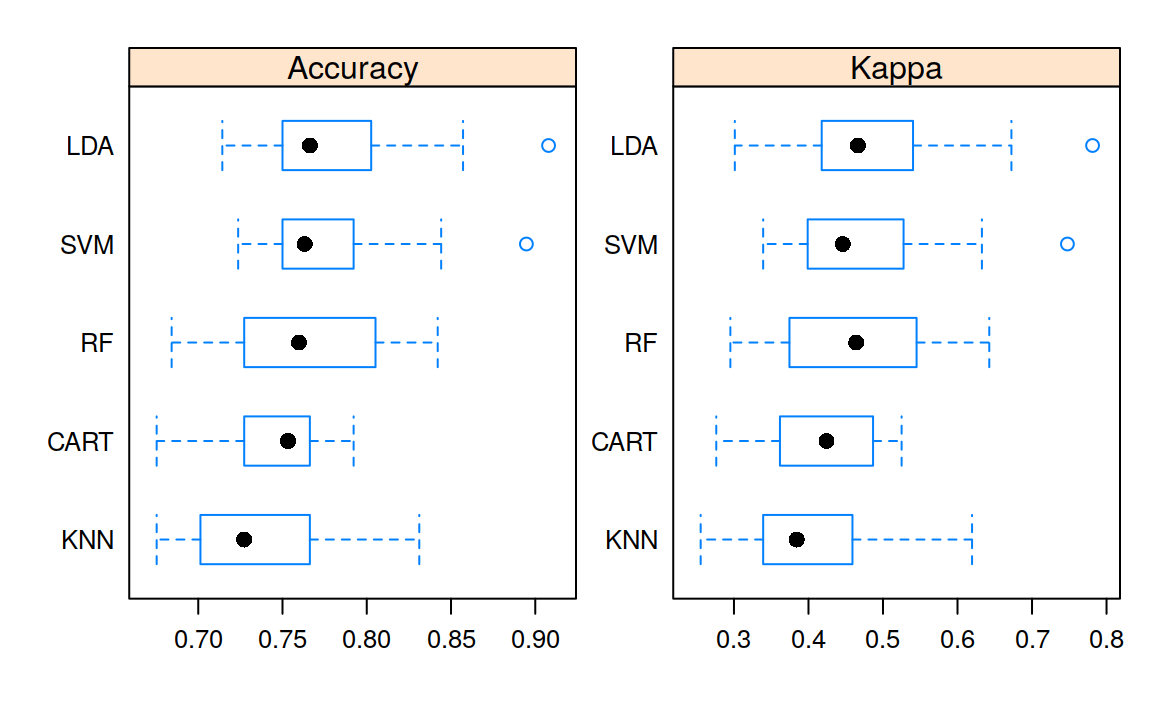
\includegraphics[width=0.7\linewidth]{comparison_342-classification_employee_attrition-lime-multi_files/figure-latex/unnamed-chunk-5-1} \end{center}

\begin{Shaded}
\begin{Highlighting}[]
\NormalTok{attrition_critical_features }\OperatorTok
\StringTok{    }\KeywordTok{ggplot}\NormalTok{(}\KeywordTok{aes}\NormalTok{(Attrition, TrainingTimesLastYear)) }\OperatorTok{+}
\StringTok{    }\KeywordTok{geom_jitter}\NormalTok{(}\DataTypeTok{alpha =} \FloatTok{0.5}\NormalTok{, }\DataTypeTok{fill =} \KeywordTok{palette_light}\NormalTok{()[[}\DecValTok{1}\NormalTok{]]) }\OperatorTok{+}
\StringTok{    }\KeywordTok{geom_violin}\NormalTok{(}\DataTypeTok{alpha =} \FloatTok{0.7}\NormalTok{, }\DataTypeTok{fill =} \KeywordTok{palette_light}\NormalTok{()[[}\DecValTok{1}\NormalTok{]]) }\OperatorTok{+}
\StringTok{    }\KeywordTok{theme_tq}\NormalTok{() }\OperatorTok{+}
\StringTok{    }\KeywordTok{labs}\NormalTok{(}
    \DataTypeTok{title =} \StringTok{"Prevalance of Training is Lower in Attrition = Yes"}\NormalTok{,}
    \DataTypeTok{subtitle =} \StringTok{"Suggests that increased training is related to lower attrition"}
\NormalTok{    )}
\end{Highlighting}
\end{Shaded}

\begin{center}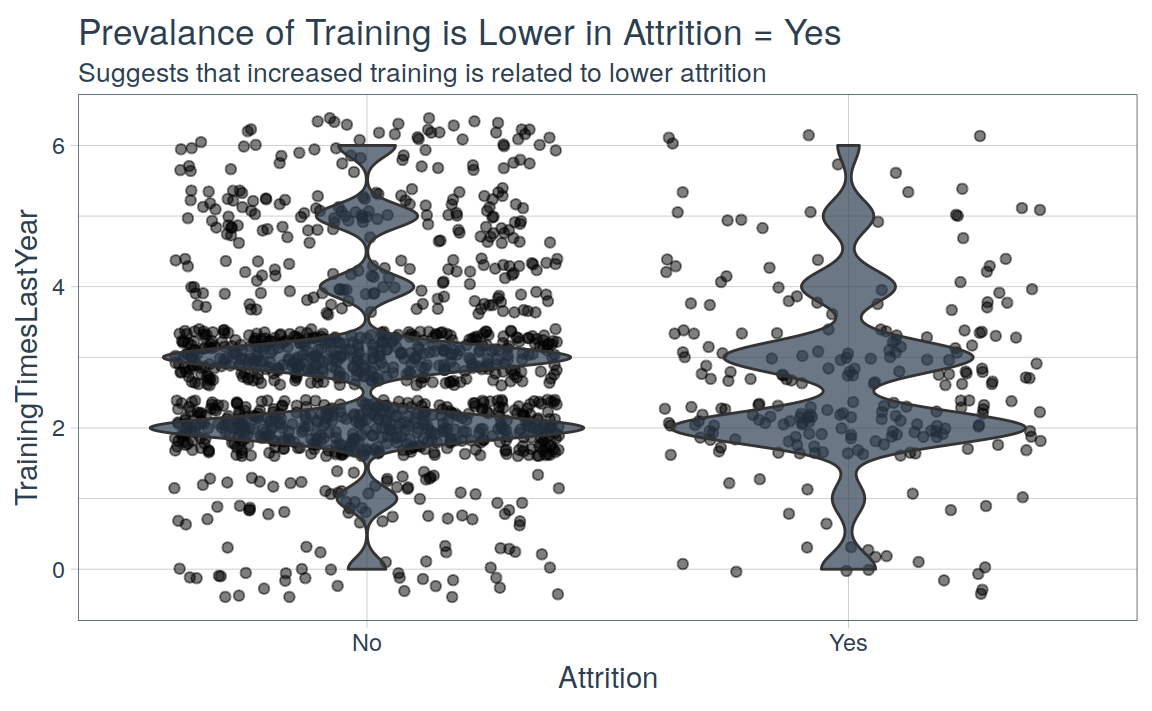
\includegraphics[width=0.7\linewidth]{comparison_342-classification_employee_attrition-lime-multi_files/figure-latex/plot-critical_training-1} \end{center}

\hypertarget{overtime}{%
\subsection{Overtime}\label{overtime}}

The plot below shows a very interesting relationship: a very high proportion of employees that turnover are working over time. The opposite is true for employees that stay.\\

\begin{Shaded}
\begin{Highlighting}[]
\NormalTok{attrition_critical_features }\OperatorTok\StringTok{ }
\StringTok{    }\KeywordTok{mutate}\NormalTok{(}\DataTypeTok{OverTime =} \KeywordTok{case_when}\NormalTok{(}
\NormalTok{                        OverTime }\OperatorTok{==}\StringTok{ "Yes"} \OperatorTok{~}\StringTok{ }\DecValTok{1}\NormalTok{,}
\NormalTok{                        OverTime }\OperatorTok{==}\StringTok{ "No"}  \OperatorTok{~}\StringTok{ }\DecValTok{0}\NormalTok{ )) }\OperatorTok\StringTok{ }
\StringTok{    }\KeywordTok{ggplot}\NormalTok{(}\KeywordTok{aes}\NormalTok{(Attrition, OverTime)) }\OperatorTok{+}
\StringTok{    }\KeywordTok{geom_jitter}\NormalTok{(}\DataTypeTok{alpha =} \FloatTok{0.5}\NormalTok{, }\DataTypeTok{fill =} \KeywordTok{palette_light}\NormalTok{()[[}\DecValTok{1}\NormalTok{]]) }\OperatorTok{+}\StringTok{ }
\StringTok{    }\KeywordTok{geom_violin}\NormalTok{(}\DataTypeTok{alpha =} \FloatTok{0.7}\NormalTok{, }\DataTypeTok{fill =} \KeywordTok{palette_light}\NormalTok{()[[}\DecValTok{1}\NormalTok{]]) }\OperatorTok{+}\StringTok{ }
\StringTok{    }\KeywordTok{theme_tq}\NormalTok{() }\OperatorTok{+}\StringTok{ }
\StringTok{    }\KeywordTok{labs}\NormalTok{(}
    \DataTypeTok{title =} \StringTok{"Prevalance of Over Time is Higher in Attrition = Yes"}\NormalTok{,}
    \DataTypeTok{subtitle =} \StringTok{"Suggests that increased overtime is related to higher attrition"}\NormalTok{)}
\end{Highlighting}
\end{Shaded}

\begin{center}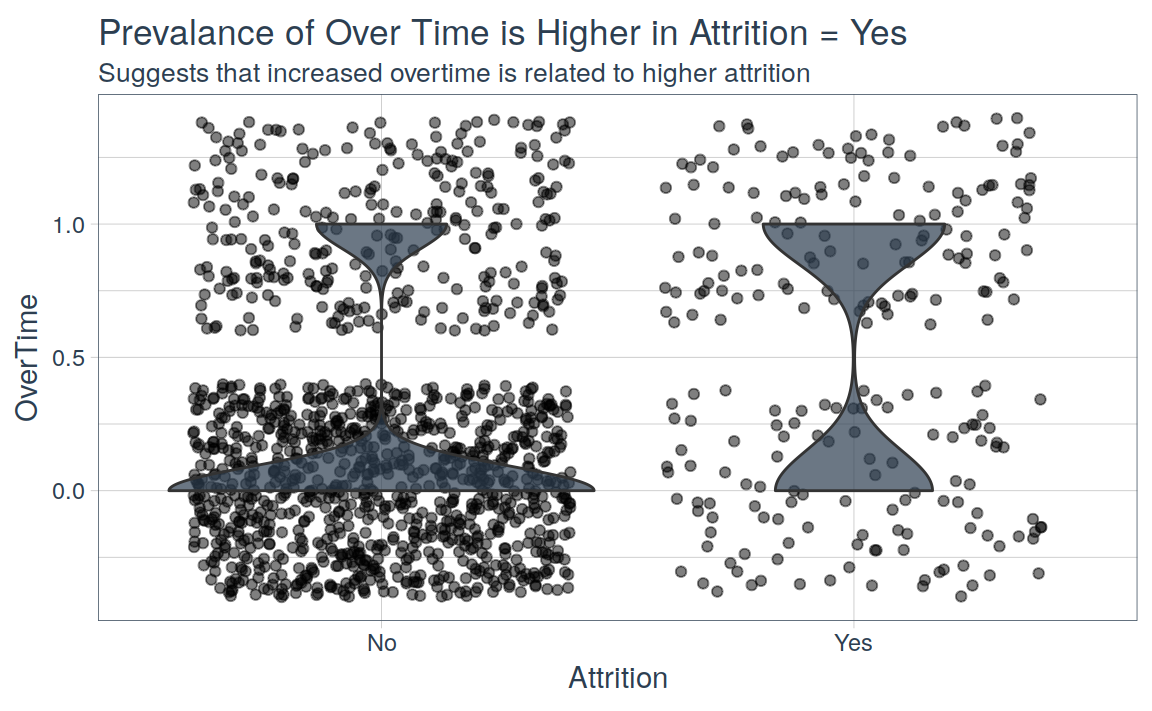
\includegraphics[width=0.7\linewidth]{comparison_342-classification_employee_attrition-lime-multi_files/figure-latex/plot-overtime-1} \end{center}

\begin{Shaded}
\begin{Highlighting}[]
\KeywordTok{ggplot}\NormalTok{(attrition_critical_features, }\KeywordTok{aes}\NormalTok{(}\DataTypeTok{x =}\NormalTok{ Attrition, }
                                        \DataTypeTok{y =}\NormalTok{ OverTime,}
\NormalTok{                                        )) }\OperatorTok{+}
\StringTok{    }\CommentTok{# geom_violin(aes(y = ..prop.., group = 1)) +}
\StringTok{    }\KeywordTok{geom_jitter}\NormalTok{(}\DataTypeTok{alpha =} \FloatTok{0.5}\NormalTok{)}
\end{Highlighting}
\end{Shaded}

\begin{center}\includegraphics[width=0.7\linewidth]{comparison_342-classification_employee_attrition-lime-multi_files/figure-latex/unnamed-chunk-6-1} \end{center}

\hypertarget{job-role}{%
\subsection{Job Role}\label{job-role}}

Several job roles are experiencing more turnover. Sales reps have the highest turnover at about 40\% followed by Lab Technician, Human Resources, Sales Executive, and Research Scientist. It may be worthwhile to investigate what localized issues could be creating the high turnover among these groups within the organization.

\begin{Shaded}
\begin{Highlighting}[]
\NormalTok{p <-}\StringTok{ }\KeywordTok{ggplot}\NormalTok{(}\DataTypeTok{data =} \KeywordTok{subset}\NormalTok{(attrition_critical_features, Attrition }\OperatorTok{==}\StringTok{ "Yes"}\NormalTok{),}
            \DataTypeTok{mapping =} \KeywordTok{aes}\NormalTok{(}\DataTypeTok{x =}\NormalTok{ JobRole))}
\NormalTok{p }\OperatorTok{+}\StringTok{ }\KeywordTok{geom_bar}\NormalTok{(}\DataTypeTok{mapping =} \KeywordTok{aes}\NormalTok{(}\DataTypeTok{y =}\NormalTok{ ..prop.., }\DataTypeTok{group =} \DecValTok{1}\NormalTok{)) }\OperatorTok{+}\StringTok{ }
\StringTok{    }\KeywordTok{coord_flip}\NormalTok{()}
\end{Highlighting}
\end{Shaded}

\begin{center}\includegraphics[width=0.7\linewidth]{comparison_342-classification_employee_attrition-lime-multi_files/figure-latex/unnamed-chunk-7-1} \end{center}

\begin{Shaded}
\begin{Highlighting}[]

\CommentTok{# geom_bar(mapping = aes(y = ..prop.., group = 1)) }
\end{Highlighting}
\end{Shaded}

\begin{Shaded}
\begin{Highlighting}[]
\NormalTok{p <-}\StringTok{ }\KeywordTok{ggplot}\NormalTok{(}\DataTypeTok{data =}\NormalTok{ attrition_critical_features,}
            \DataTypeTok{mapping =} \KeywordTok{aes}\NormalTok{(}\DataTypeTok{x =}\NormalTok{ JobRole))}
\NormalTok{p }\OperatorTok{+}\StringTok{ }\KeywordTok{geom_bar}\NormalTok{(}\DataTypeTok{mapping =} \KeywordTok{aes}\NormalTok{(}\DataTypeTok{y =}\NormalTok{ ..prop.., }\DataTypeTok{group =} \DecValTok{1}\NormalTok{)) }\OperatorTok{+}\StringTok{ }
\StringTok{    }\KeywordTok{coord_flip}\NormalTok{() }\OperatorTok{+}
\StringTok{    }\KeywordTok{facet_wrap}\NormalTok{(Attrition }\OperatorTok{~}\StringTok{ }\NormalTok{.)}
\end{Highlighting}
\end{Shaded}

\begin{center}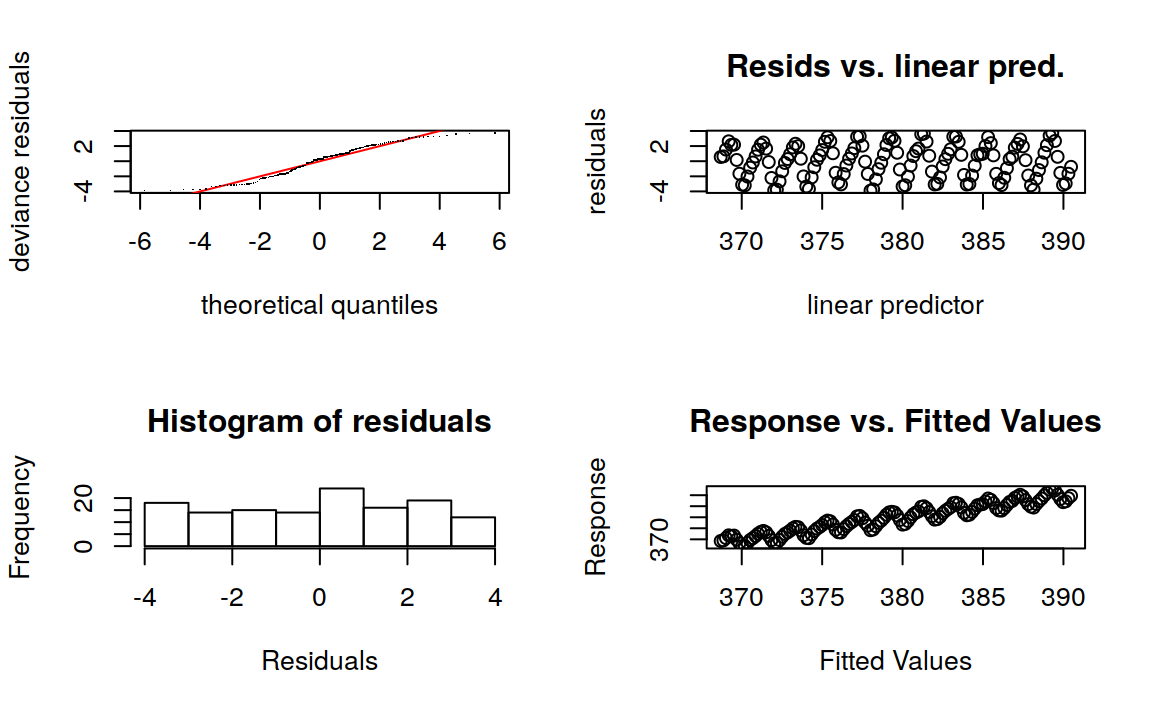
\includegraphics[width=0.7\linewidth]{comparison_342-classification_employee_attrition-lime-multi_files/figure-latex/unnamed-chunk-8-1} \end{center}

\begin{Shaded}
\begin{Highlighting}[]
\NormalTok{attrition_critical_features }\OperatorTok
\StringTok{    }\KeywordTok{group_by}\NormalTok{(JobRole, Attrition) }\OperatorTok\StringTok{ }
\StringTok{    }\KeywordTok{summarize}\NormalTok{(}\DataTypeTok{total =} \KeywordTok{n}\NormalTok{())}
\CommentTok{#> # A tibble: 18 x 3}
\CommentTok{#> # Groups:   JobRole [9]}
\CommentTok{#>   JobRole                   Attrition total}
\CommentTok{#>   <fct>                     <fct>     <int>}
\CommentTok{#> 1 Healthcare Representative No          122}
\CommentTok{#> 2 Healthcare Representative Yes           9}
\CommentTok{#> 3 Human Resources           No           40}
\CommentTok{#> 4 Human Resources           Yes          12}
\CommentTok{#> 5 Laboratory Technician     No          197}
\CommentTok{#> 6 Laboratory Technician     Yes          62}
\CommentTok{#> # ... with 12 more rows}
\end{Highlighting}
\end{Shaded}

\begin{Shaded}
\begin{Highlighting}[]
\NormalTok{attrition_critical_features }\OperatorTok
\StringTok{    }\KeywordTok{group_by}\NormalTok{(JobRole, Attrition) }\OperatorTok\StringTok{ }
\StringTok{    }\KeywordTok{summarize}\NormalTok{(}\DataTypeTok{total =} \KeywordTok{n}\NormalTok{()) }\OperatorTok\StringTok{ }
\StringTok{    }\KeywordTok{spread}\NormalTok{(}\DataTypeTok{key =}\NormalTok{ Attrition, }\DataTypeTok{value =}\NormalTok{ total) }\OperatorTok\StringTok{ }
\StringTok{    }\KeywordTok{mutate}\NormalTok{(}\DataTypeTok{pct_attrition =}\NormalTok{ Yes }\OperatorTok{/}\StringTok{ }\NormalTok{(Yes }\OperatorTok{+}\StringTok{ }\NormalTok{No))}
\CommentTok{#> # A tibble: 9 x 4}
\CommentTok{#> # Groups:   JobRole [9]}
\CommentTok{#>   JobRole                      No   Yes pct_attrition}
\CommentTok{#>   <fct>                     <int> <int>         <dbl>}
\CommentTok{#> 1 Healthcare Representative   122     9        0.0687}
\CommentTok{#> 2 Human Resources              40    12        0.231 }
\CommentTok{#> 3 Laboratory Technician       197    62        0.239 }
\CommentTok{#> 4 Manager                      97     5        0.0490}
\CommentTok{#> 5 Manufacturing Director      135    10        0.0690}
\CommentTok{#> 6 Research Director            78     2        0.025 }
\CommentTok{#> # ... with 3 more rows}
\end{Highlighting}
\end{Shaded}

\begin{Shaded}
\begin{Highlighting}[]
\NormalTok{attrition_critical_features }\OperatorTok
\StringTok{    }\KeywordTok{group_by}\NormalTok{(JobRole, Attrition) }\OperatorTok\StringTok{ }
\StringTok{    }\KeywordTok{summarize}\NormalTok{(}\DataTypeTok{total =} \KeywordTok{n}\NormalTok{()) }\OperatorTok
\StringTok{    }\KeywordTok{spread}\NormalTok{(}\DataTypeTok{key =}\NormalTok{ Attrition, }\DataTypeTok{value =}\NormalTok{ total) }\OperatorTok
\StringTok{    }\KeywordTok{mutate}\NormalTok{(}\DataTypeTok{pct_attrition =}\NormalTok{ Yes }\OperatorTok{/}\StringTok{ }\NormalTok{(Yes }\OperatorTok{+}\StringTok{ }\NormalTok{No)) }\OperatorTok
\StringTok{    }\KeywordTok{ggplot}\NormalTok{(}\KeywordTok{aes}\NormalTok{(}\DataTypeTok{x =}\NormalTok{ forcats}\OperatorTok{::}\KeywordTok{fct_reorder}\NormalTok{(JobRole, pct_attrition), }\DataTypeTok{y =}\NormalTok{ pct_attrition)) }\OperatorTok{+}
\StringTok{    }\KeywordTok{geom_bar}\NormalTok{(}\DataTypeTok{stat =} \StringTok{"identity"}\NormalTok{, }\DataTypeTok{alpha =} \DecValTok{1}\NormalTok{, }\DataTypeTok{fill =} \KeywordTok{palette_light}\NormalTok{()[[}\DecValTok{1}\NormalTok{]]) }\OperatorTok{+}
\StringTok{    }\KeywordTok{expand_limits}\NormalTok{(}\DataTypeTok{y =} \KeywordTok{c}\NormalTok{(}\DecValTok{0}\NormalTok{, }\DecValTok{1}\NormalTok{)) }\OperatorTok{+}
\StringTok{    }\KeywordTok{coord_flip}\NormalTok{() }\OperatorTok{+}
\StringTok{    }\KeywordTok{theme_tq}\NormalTok{() }\OperatorTok{+}
\StringTok{    }\KeywordTok{labs}\NormalTok{(}
        \DataTypeTok{title =} \StringTok{"Attrition Varies By Job Role"}\NormalTok{,}
        \DataTypeTok{subtitle =} \StringTok{"Sales Rep, Lab Tech, HR, Sales Exec, and Research Scientist }
\StringTok{        have much higher turnover"}\NormalTok{,}
        \DataTypeTok{y =} \StringTok{"Attrition Percentage (Yes / Total)"}\NormalTok{,}
        \DataTypeTok{x =} \StringTok{"JobRole"}
\NormalTok{    )}
\end{Highlighting}
\end{Shaded}

\begin{center}\includegraphics[width=0.7\linewidth]{comparison_342-classification_employee_attrition-lime-multi_files/figure-latex/unnamed-chunk-11-1} \end{center}

\hypertarget{conclusions}{%
\section{Conclusions}\label{conclusions}}

There's a lot to take away from this article. We showed how you can use predictive analytics to develop sophisticated models that very accurately detect employees that are at risk of turnover. The autoML algorithm from H2O.ai worked well for classifying attrition with an accuracy around 87\% on unseen / unmodeled data. We then used LIME to breakdown the complex ensemble model returned from H2O into critical features that are related to attrition. Overall, this is a really useful example where we can see how machine learning and data science can be used in business applications.

\hypertarget{dealing-with-unbalanced-data}{%
\chapter{Dealing with unbalanced data}\label{dealing-with-unbalanced-data}}

\hypertarget{breast-cancer-dataset}{%
\section{Breast cancer dataset}\label{breast-cancer-dataset}}

\hypertarget{introduction-1}{%
\section{Introduction}\label{introduction-1}}

Source: \url{https://shiring.github.io/machine_learning/2017/04/02/unbalanced}

\begin{Shaded}
\begin{Highlighting}[]
\KeywordTok{library}\NormalTok{(caret)}
\CommentTok{#> Loading required package: lattice}
\CommentTok{#> Loading required package: ggplot2}
\CommentTok{#> Registered S3 methods overwritten by 'ggplot2':}
\CommentTok{#>   method         from }
\CommentTok{#>   [.quosures     rlang}
\CommentTok{#>   c.quosures     rlang}
\CommentTok{#>   print.quosures rlang}
\KeywordTok{library}\NormalTok{(mice)}
\CommentTok{#> }
\CommentTok{#> Attaching package: 'mice'}
\CommentTok{#> The following objects are masked from 'package:base':}
\CommentTok{#> }
\CommentTok{#>     cbind, rbind}
\KeywordTok{library}\NormalTok{(ggplot2)}
\end{Highlighting}
\end{Shaded}

In my last post, where I shared the code that I used to produce an example analysis to go along with my webinar on building meaningful models for disease prediction, I mentioned that it is advised to consider over- or under-sampling when you have unbalanced data sets. Because my focus in this webinar was on evaluating model performance, I did not want to add an additional layer of complexity and therefore did not further discuss how to specifically deal with unbalanced data.

But because I had gotten a few questions regarding this, I thought it would be worthwhile to explain over- and under-sampling techniques in more detail and show how you can very easily implement them with \texttt{caret}.

\hypertarget{read-and-process-the-data}{%
\section{Read and process the data}\label{read-and-process-the-data}}

\begin{Shaded}
\begin{Highlighting}[]
\NormalTok{bc_data <-}\StringTok{ }\KeywordTok{read.table}\NormalTok{(}\KeywordTok{file.path}\NormalTok{(data_raw_dir, }\StringTok{"breast-cancer-wisconsin.data"}\NormalTok{), }
                      \DataTypeTok{header =} \OtherTok{FALSE}\NormalTok{, }\DataTypeTok{sep =} \StringTok{","}\NormalTok{)}

\KeywordTok{colnames}\NormalTok{(bc_data) <-}\StringTok{ }\KeywordTok{c}\NormalTok{(}\StringTok{"sample_code_number"}\NormalTok{, }\StringTok{"clump_thickness"}\NormalTok{, }
                       \StringTok{"uniformity_of_cell_size"}\NormalTok{, }\StringTok{"uniformity_of_cell_shape"}\NormalTok{,}
                       \StringTok{"marginal_adhesion"}\NormalTok{, }\StringTok{"single_epithelial_cell_size"}\NormalTok{, }
                       \StringTok{"bare_nuclei"}\NormalTok{, }\StringTok{"bland_chromatin"}\NormalTok{, }\StringTok{"normal_nucleoli"}\NormalTok{, }
                       \StringTok{"mitosis"}\NormalTok{, }\StringTok{"classes"}\NormalTok{)}

\NormalTok{bc_data}\OperatorTok{$}\NormalTok{classes <-}\StringTok{ }\KeywordTok{ifelse}\NormalTok{(bc_data}\OperatorTok{$}\NormalTok{classes }\OperatorTok{==}\StringTok{ "2"}\NormalTok{, }\StringTok{"benign"}\NormalTok{,}
                          \KeywordTok{ifelse}\NormalTok{(bc_data}\OperatorTok{$}\NormalTok{classes }\OperatorTok{==}\StringTok{ "4"}\NormalTok{, }\StringTok{"malignant"}\NormalTok{, }\OtherTok{NA}\NormalTok{))}

\NormalTok{bc_data[bc_data }\OperatorTok{==}\StringTok{ "?"}\NormalTok{] <-}\StringTok{ }\OtherTok{NA}

\CommentTok{# how many NAs are in the data}
\KeywordTok{length}\NormalTok{(}\KeywordTok{which}\NormalTok{(}\KeywordTok{is.na}\NormalTok{(bc_data)))}
\CommentTok{#> [1] 16}
\end{Highlighting}
\end{Shaded}

\begin{Shaded}
\begin{Highlighting}[]
\CommentTok{# impute missing data}

\CommentTok{# skip columns: sample_code_number and classes}
\NormalTok{bc_data[,}\DecValTok{2}\OperatorTok{:}\DecValTok{10}\NormalTok{] <-}\StringTok{ }\KeywordTok{apply}\NormalTok{(bc_data[, }\DecValTok{2}\OperatorTok{:}\DecValTok{10}\NormalTok{], }\DecValTok{2}\NormalTok{, }\ControlFlowTok{function}\NormalTok{(x) }\KeywordTok{as.numeric}\NormalTok{(}\KeywordTok{as.character}\NormalTok{(x)))}

\CommentTok{# impute but stay mute}
\NormalTok{dataset_impute <-}\StringTok{ }\KeywordTok{mice}\NormalTok{(bc_data[, }\DecValTok{2}\OperatorTok{:}\DecValTok{10}\NormalTok{],  }\DataTypeTok{print =} \OtherTok{FALSE}\NormalTok{)}

\CommentTok{# bind "classes" with the rest. skip "sample_code_number"}
\NormalTok{bc_data <-}\StringTok{ }\KeywordTok{cbind}\NormalTok{(bc_data[, }\DecValTok{11}\NormalTok{, }\DataTypeTok{drop =} \OtherTok{FALSE}\NormalTok{], }
\NormalTok{                 mice}\OperatorTok{::}\KeywordTok{complete}\NormalTok{(dataset_impute, }\DataTypeTok{action =} \DecValTok{1}\NormalTok{))}

\NormalTok{bc_data}\OperatorTok{$}\NormalTok{classes <-}\StringTok{ }\KeywordTok{as.factor}\NormalTok{(bc_data}\OperatorTok{$}\NormalTok{classes)}
\end{Highlighting}
\end{Shaded}

\hypertarget{unbalanced-data}{%
\subsection{Unbalanced data}\label{unbalanced-data}}

In this context, unbalanced data refers to classification problems where we have unequal instances for different classes. Having unbalanced data is actually very common in general, but it is especially prevalent when working with disease data where we usually have more healthy control samples than disease cases. Even more extreme unbalance is seen with fraud detection, where e.g.~most credit card uses are okay and only very few will be fraudulent. In the example I used for my webinar, a \emph{breast cancer} dataset, we had about twice as many benign than malignant samples.

\begin{Shaded}
\begin{Highlighting}[]
\CommentTok{# how many benign and malignant cases are there?}
\KeywordTok{summary}\NormalTok{(bc_data}\OperatorTok{$}\NormalTok{classes)}
\CommentTok{#>    benign malignant }
\CommentTok{#>       458       241}
\end{Highlighting}
\end{Shaded}

\hypertarget{why-is-unbalanced-data-a-problem-in-machine-learning}{%
\subsubsection{Why is unbalanced data a problem in machine learning?}\label{why-is-unbalanced-data-a-problem-in-machine-learning}}

Most machine learning classification algorithms are sensitive to unbalance in the predictor classes. Let's consider an even more extreme example than our breast cancer dataset: assume we had 10 malignant vs 90 benign samples. A machine learning model that has been trained and tested on such a dataset could now predict ``benign'' for all samples and still gain a very high accuracy. An unbalanced dataset will bias the prediction model towards the more common class!

\hypertarget{how-to-balance-data-for-modeling}{%
\subsubsection{How to balance data for modeling}\label{how-to-balance-data-for-modeling}}

The basic theoretical concepts behind over- and under-sampling are very simple:

With under-sampling, we randomly select a subset of samples from the class with more instances to match the number of samples coming from each class. In our example, we would randomly pick 241 out of the 458 benign cases. The main disadvantage of under-sampling is that we lose potentially relevant information from the left-out samples.

With oversampling, we randomly duplicate samples from the class with fewer instances or we generate additional instances based on the data that we have, so as to match the number of samples in each class. While we avoid losing information with this approach, we also run the risk of overfitting our model as we are more likely to get the same samples in the training and in the test data, i.e.~the test data is no longer independent from training data. This would lead to an overestimation of our model's performance and generalizability.

In reality though, we should not simply perform over- or under-sampling on our training data and then run the model. We need to account for cross-validation and perform over- or under-sampling on each fold independently to get an honest estimate of model performance!

\hypertarget{modeling-the-original-unbalanced-data}{%
\subsubsection{Modeling the original unbalanced data}\label{modeling-the-original-unbalanced-data}}

Here is the same model I used in my webinar example: I randomly divide the data into training and test sets (stratified by class) and perform Random Forest modeling with 10 x 10 repeated cross-validation. Final model performance is then measured on the test set.

\begin{Shaded}
\begin{Highlighting}[]
\KeywordTok{set.seed}\NormalTok{(}\DecValTok{42}\NormalTok{)}
\NormalTok{index <-}\StringTok{ }\KeywordTok{createDataPartition}\NormalTok{(bc_data}\OperatorTok{$}\NormalTok{classes, }\DataTypeTok{p =} \FloatTok{0.7}\NormalTok{, }\DataTypeTok{list =} \OtherTok{FALSE}\NormalTok{)}
\NormalTok{train_data <-}\StringTok{ }\NormalTok{bc_data[index, ]}
\NormalTok{test_data  <-}\StringTok{ }\NormalTok{bc_data[}\OperatorTok{-}\NormalTok{index, ]}
\end{Highlighting}
\end{Shaded}

\begin{Shaded}
\begin{Highlighting}[]
\KeywordTok{set.seed}\NormalTok{(}\DecValTok{42}\NormalTok{)}
\NormalTok{model_rf <-}\StringTok{ }\NormalTok{caret}\OperatorTok{::}\KeywordTok{train}\NormalTok{(classes }\OperatorTok{~}\StringTok{ }\NormalTok{.,}
                         \DataTypeTok{data =}\NormalTok{ train_data,}
                         \DataTypeTok{method =} \StringTok{"rf"}\NormalTok{,}
                         \DataTypeTok{preProcess =} \KeywordTok{c}\NormalTok{(}\StringTok{"scale"}\NormalTok{, }\StringTok{"center"}\NormalTok{),}
                         \DataTypeTok{trControl =} \KeywordTok{trainControl}\NormalTok{(}\DataTypeTok{method =} \StringTok{"repeatedcv"}\NormalTok{, }
                                                  \DataTypeTok{number =} \DecValTok{10}\NormalTok{, }
                                                  \DataTypeTok{repeats =} \DecValTok{10}\NormalTok{, }
                                                  \DataTypeTok{verboseIter =} \OtherTok{FALSE}\NormalTok{))}
\end{Highlighting}
\end{Shaded}

\begin{Shaded}
\begin{Highlighting}[]
\NormalTok{final <-}\StringTok{ }\KeywordTok{data.frame}\NormalTok{(}\DataTypeTok{actual =}\NormalTok{ test_data}\OperatorTok{$}\NormalTok{classes,}
                    \KeywordTok{predict}\NormalTok{(model_rf, }
                            \DataTypeTok{newdata =}\NormalTok{ test_data, }
                            \DataTypeTok{type =} \StringTok{"prob"}\NormalTok{))}

\NormalTok{final}\OperatorTok{$}\NormalTok{predict <-}\StringTok{ }\KeywordTok{ifelse}\NormalTok{(final}\OperatorTok{$}\NormalTok{benign }\OperatorTok{>}\StringTok{ }\FloatTok{0.5}\NormalTok{, }\StringTok{"benign"}\NormalTok{, }\StringTok{"malignant"}\NormalTok{)}
\end{Highlighting}
\end{Shaded}

\begin{Shaded}
\begin{Highlighting}[]
\NormalTok{final_predict <-}\StringTok{ }\KeywordTok{as.factor}\NormalTok{(final}\OperatorTok{$}\NormalTok{predict)}
\NormalTok{test_data_classes <-}\StringTok{ }\KeywordTok{as.factor}\NormalTok{(test_data}\OperatorTok{$}\NormalTok{classes)}

\NormalTok{cm_original <-}\StringTok{ }\KeywordTok{confusionMatrix}\NormalTok{(final_predict, test_data_classes)}
\NormalTok{cm_original}\OperatorTok{$}\NormalTok{byClass[}\StringTok{'Sensitivity'}\NormalTok{]}
\CommentTok{#> Sensitivity }
\CommentTok{#>       0.978}
\end{Highlighting}
\end{Shaded}

\hypertarget{under-sampling}{%
\section{Under-sampling}\label{under-sampling}}

Luckily, \texttt{caret} makes it very easy to incorporate over- and under-sampling techniques with cross-validation resampling. We can simply add the sampling option to our \texttt{trainControl} and choose down for under- (also called \texttt{down}-) sampling. The rest stays the same as with our original model.

\begin{Shaded}
\begin{Highlighting}[]
\KeywordTok{set.seed}\NormalTok{(}\DecValTok{42}\NormalTok{)}
\NormalTok{ctrl <-}\StringTok{ }\KeywordTok{trainControl}\NormalTok{(}\DataTypeTok{method =} \StringTok{"repeatedcv"}\NormalTok{, }
                     \DataTypeTok{number =} \DecValTok{10}\NormalTok{, }
                     \DataTypeTok{repeats =} \DecValTok{10}\NormalTok{, }
                     \DataTypeTok{verboseIter =} \OtherTok{FALSE}\NormalTok{,}
                     \DataTypeTok{sampling =} \StringTok{"down"}\NormalTok{)}


\NormalTok{model_rf_under <-}\StringTok{ }\NormalTok{caret}\OperatorTok{::}\KeywordTok{train}\NormalTok{(classes }\OperatorTok{~}\StringTok{ }\NormalTok{.,}
                         \DataTypeTok{data =}\NormalTok{ train_data,}
                         \DataTypeTok{method =} \StringTok{"rf"}\NormalTok{,}
                         \DataTypeTok{preProcess =} \KeywordTok{c}\NormalTok{(}\StringTok{"scale"}\NormalTok{, }\StringTok{"center"}\NormalTok{),}
                         \DataTypeTok{trControl =}\NormalTok{ ctrl)}
\end{Highlighting}
\end{Shaded}

\begin{Shaded}
\begin{Highlighting}[]
\NormalTok{final_under <-}\StringTok{ }\KeywordTok{data.frame}\NormalTok{(}\DataTypeTok{actual =}\NormalTok{ test_data}\OperatorTok{$}\NormalTok{classes,}
                    \KeywordTok{predict}\NormalTok{(model_rf_under, }
                            \DataTypeTok{newdata =}\NormalTok{ test_data, }
                            \DataTypeTok{type =} \StringTok{"prob"}\NormalTok{))}

\NormalTok{final_under}\OperatorTok{$}\NormalTok{predict <-}\StringTok{ }\KeywordTok{ifelse}\NormalTok{(final_under}\OperatorTok{$}\NormalTok{benign }\OperatorTok{>}\StringTok{ }\FloatTok{0.5}\NormalTok{, }\StringTok{"benign"}\NormalTok{, }\StringTok{"malignant"}\NormalTok{)}
\end{Highlighting}
\end{Shaded}

\begin{Shaded}
\begin{Highlighting}[]
\NormalTok{final_under_predict <-}\StringTok{ }\KeywordTok{as.factor}\NormalTok{(final_under}\OperatorTok{$}\NormalTok{predict)}
\NormalTok{test_data_classes <-}\StringTok{ }\NormalTok{test_data}\OperatorTok{$}\NormalTok{classes}

\NormalTok{cm_under <-}\StringTok{ }\KeywordTok{confusionMatrix}\NormalTok{(final_under_predict, test_data_classes)}
\NormalTok{cm_under}\OperatorTok{$}\NormalTok{byClass[}\StringTok{'Sensitivity'}\NormalTok{]}
\CommentTok{#> Sensitivity }
\CommentTok{#>       0.978}
\end{Highlighting}
\end{Shaded}

\hypertarget{oversampling}{%
\section{Oversampling}\label{oversampling}}

For over- (also called up-) sampling we simply specify sampling = ``up''.

\begin{Shaded}
\begin{Highlighting}[]
\KeywordTok{set.seed}\NormalTok{(}\DecValTok{42}\NormalTok{)}
\NormalTok{ctrl <-}\StringTok{ }\KeywordTok{trainControl}\NormalTok{(}\DataTypeTok{method =} \StringTok{"repeatedcv"}\NormalTok{, }
                     \DataTypeTok{number =} \DecValTok{10}\NormalTok{, }
                     \DataTypeTok{repeats =} \DecValTok{10}\NormalTok{, }
                     \DataTypeTok{verboseIter =} \OtherTok{FALSE}\NormalTok{,}
                     \DataTypeTok{sampling =} \StringTok{"up"}\NormalTok{)}


\NormalTok{model_rf_over <-}\StringTok{ }\NormalTok{caret}\OperatorTok{::}\KeywordTok{train}\NormalTok{(classes }\OperatorTok{~}\StringTok{ }\NormalTok{.,}
                         \DataTypeTok{data =}\NormalTok{ train_data,}
                         \DataTypeTok{method =} \StringTok{"rf"}\NormalTok{,}
                         \DataTypeTok{preProcess =} \KeywordTok{c}\NormalTok{(}\StringTok{"scale"}\NormalTok{, }\StringTok{"center"}\NormalTok{),}
                         \DataTypeTok{trControl =}\NormalTok{ ctrl)}
\end{Highlighting}
\end{Shaded}

\begin{Shaded}
\begin{Highlighting}[]
\NormalTok{final_over <-}\StringTok{ }\KeywordTok{data.frame}\NormalTok{(}\DataTypeTok{actual =}\NormalTok{ test_data}\OperatorTok{$}\NormalTok{classes,}
                          \KeywordTok{predict}\NormalTok{(model_rf_over, }
                                  \DataTypeTok{newdata =}\NormalTok{ test_data, }
                                  \DataTypeTok{type =} \StringTok{"prob"}\NormalTok{))}

\NormalTok{final_over}\OperatorTok{$}\NormalTok{predict <-}\StringTok{ }\KeywordTok{ifelse}\NormalTok{(final_over}\OperatorTok{$}\NormalTok{benign }\OperatorTok{>}\StringTok{ }\FloatTok{0.5}\NormalTok{, }\StringTok{"benign"}\NormalTok{, }\StringTok{"malignant"}\NormalTok{)}
\end{Highlighting}
\end{Shaded}

\begin{Shaded}
\begin{Highlighting}[]
\NormalTok{final_over_predict <-}\StringTok{ }\KeywordTok{as.factor}\NormalTok{(final_over}\OperatorTok{$}\NormalTok{predict)}
\NormalTok{test_data_classes <-}\StringTok{ }\NormalTok{test_data}\OperatorTok{$}\NormalTok{classes}

\NormalTok{cm_over <-}\StringTok{ }\KeywordTok{confusionMatrix}\NormalTok{(final_over_predict, test_data_classes)}
\NormalTok{cm_over}\OperatorTok{$}\NormalTok{byClass[}\StringTok{'Sensitivity'}\NormalTok{]}
\CommentTok{#> Sensitivity }
\CommentTok{#>       0.978}
\end{Highlighting}
\end{Shaded}

\hypertarget{rose}{%
\subsection{ROSE}\label{rose}}

Besides over- and under-sampling, there are hybrid methods that combine under-sampling with the generation of additional data. Two of the most popular are ROSE and SMOTE.

\begin{quote}
From Nicola Lunardon, Giovanna Menardi and Nicola Torelli's ``ROSE: A Package for Binary Imbalanced Learning'' (R Journal, 2014, Vol. 6 Issue 1, p.~79): ``The ROSE package provides functions to deal with binary classification problems in the presence of imbalanced classes. Artificial balanced samples are generated according to a smoothed bootstrap approach and allow for aiding both the phases of estimation and accuracy evaluation of a binary classifier in the presence of a rare class. Functions that implement more traditional remedies for the class imbalance and different metrics to evaluate accuracy are also provided. These are estimated by holdout, bootstrap, or cross-validation methods.''
\end{quote}

You implement them the same way as before, this time choosing sampling = ``rose''\ldots{}

\begin{Shaded}
\begin{Highlighting}[]
\KeywordTok{set.seed}\NormalTok{(}\DecValTok{42}\NormalTok{)}
\NormalTok{ctrl <-}\StringTok{ }\KeywordTok{trainControl}\NormalTok{(}\DataTypeTok{method =} \StringTok{"repeatedcv"}\NormalTok{, }
                     \DataTypeTok{number =} \DecValTok{10}\NormalTok{, }
                     \DataTypeTok{repeats =} \DecValTok{10}\NormalTok{, }
                     \DataTypeTok{verboseIter =} \OtherTok{FALSE}\NormalTok{,}
                     \DataTypeTok{sampling =} \StringTok{"rose"}\NormalTok{)}

\NormalTok{model_rf_rose <-}\StringTok{ }\NormalTok{caret}\OperatorTok{::}\KeywordTok{train}\NormalTok{(classes }\OperatorTok{~}\StringTok{ }\NormalTok{.,}
                              \DataTypeTok{data =}\NormalTok{ train_data,}
                              \DataTypeTok{method =} \StringTok{"rf"}\NormalTok{,}
                              \DataTypeTok{preProcess =} \KeywordTok{c}\NormalTok{(}\StringTok{"scale"}\NormalTok{, }\StringTok{"center"}\NormalTok{),}
                              \DataTypeTok{trControl =}\NormalTok{ ctrl)}
\CommentTok{#> Loaded ROSE 0.0-3}
\end{Highlighting}
\end{Shaded}

\begin{Shaded}
\begin{Highlighting}[]
\NormalTok{final_rose <-}\StringTok{ }\KeywordTok{data.frame}\NormalTok{(}\DataTypeTok{actual =}\NormalTok{ test_data}\OperatorTok{$}\NormalTok{classes,}
                         \KeywordTok{predict}\NormalTok{(model_rf_rose, }
                                 \DataTypeTok{newdata =}\NormalTok{ test_data, }
                                 \DataTypeTok{type =} \StringTok{"prob"}\NormalTok{))}

\NormalTok{final_rose}\OperatorTok{$}\NormalTok{predict <-}\StringTok{ }\KeywordTok{ifelse}\NormalTok{(final_rose}\OperatorTok{$}\NormalTok{benign }\OperatorTok{>}\StringTok{ }\FloatTok{0.5}\NormalTok{, }\StringTok{"benign"}\NormalTok{, }\StringTok{"malignant"}\NormalTok{)}
\end{Highlighting}
\end{Shaded}

\begin{Shaded}
\begin{Highlighting}[]
\NormalTok{cm_rose <-}\StringTok{ }\KeywordTok{confusionMatrix}\NormalTok{(}\KeywordTok{as.factor}\NormalTok{(final_rose}\OperatorTok{$}\NormalTok{predict), }
                           \KeywordTok{as.factor}\NormalTok{(test_data}\OperatorTok{$}\NormalTok{classes))}
\NormalTok{cm_rose}\OperatorTok{$}\NormalTok{byClass[}\StringTok{'Sensitivity'}\NormalTok{]}
\CommentTok{#> Sensitivity }
\CommentTok{#>       0.985}
\end{Highlighting}
\end{Shaded}

\hypertarget{smote}{%
\subsection{SMOTE}\label{smote}}

\ldots{} or by choosing sampling = ``smote'' in the \texttt{trainControl} settings.

\begin{quote}
From Nitesh V. Chawla, Kevin W. Bowyer, Lawrence O. Hall and W. Philip Kegelmeyer's ``SMOTE: Synthetic Minority Over-sampling Technique'' (Journal of Artificial Intelligence Research, 2002, Vol. 16, pp.~321--357): ``This paper shows that a combination of our method of over-sampling the minority (abnormal) class and under-sampling the majority (normal) class can achieve better classifier performance (in ROC space) than only under-sampling the majority class. This paper also shows that a combination of our method of over-sampling the minority class and under-sampling the majority class can achieve better classifier performance (in ROC space) than varying the loss ratios in Ripper or class priors in Naive Bayes. Our method of over-sampling the minority class involves creating synthetic minority class examples.''
\end{quote}

\begin{Shaded}
\begin{Highlighting}[]
\KeywordTok{set.seed}\NormalTok{(}\DecValTok{42}\NormalTok{)}
\NormalTok{ctrl <-}\StringTok{ }\KeywordTok{trainControl}\NormalTok{(}\DataTypeTok{method =} \StringTok{"repeatedcv"}\NormalTok{, }
                     \DataTypeTok{number =} \DecValTok{10}\NormalTok{, }
                     \DataTypeTok{repeats =} \DecValTok{10}\NormalTok{, }
                     \DataTypeTok{verboseIter =} \OtherTok{FALSE}\NormalTok{,}
                     \DataTypeTok{sampling =} \StringTok{"smote"}\NormalTok{)}

\NormalTok{model_rf_smote <-}\StringTok{ }\NormalTok{caret}\OperatorTok{::}\KeywordTok{train}\NormalTok{(classes }\OperatorTok{~}\StringTok{ }\NormalTok{.,}
                              \DataTypeTok{data =}\NormalTok{ train_data,}
                              \DataTypeTok{method =} \StringTok{"rf"}\NormalTok{,}
                              \DataTypeTok{preProcess =} \KeywordTok{c}\NormalTok{(}\StringTok{"scale"}\NormalTok{, }\StringTok{"center"}\NormalTok{),}
                              \DataTypeTok{trControl =}\NormalTok{ ctrl)}
\CommentTok{#> Loading required package: grid}
\CommentTok{#> Registered S3 method overwritten by 'xts':}
\CommentTok{#>   method     from}
\CommentTok{#>   as.zoo.xts zoo}
\CommentTok{#> Registered S3 method overwritten by 'quantmod':}
\CommentTok{#>   method            from}
\CommentTok{#>   as.zoo.data.frame zoo}
\end{Highlighting}
\end{Shaded}

\begin{Shaded}
\begin{Highlighting}[]
\NormalTok{final_smote <-}\StringTok{ }\KeywordTok{data.frame}\NormalTok{(}\DataTypeTok{actual =}\NormalTok{ test_data}\OperatorTok{$}\NormalTok{classes,}
                         \KeywordTok{predict}\NormalTok{(model_rf_smote, }
                                 \DataTypeTok{newdata =}\NormalTok{ test_data, }
                                 \DataTypeTok{type =} \StringTok{"prob"}\NormalTok{))}

\NormalTok{final_smote}\OperatorTok{$}\NormalTok{predict <-}\StringTok{ }\KeywordTok{ifelse}\NormalTok{(final_smote}\OperatorTok{$}\NormalTok{benign }\OperatorTok{>}\StringTok{ }\FloatTok{0.5}\NormalTok{, }\StringTok{"benign"}\NormalTok{, }\StringTok{"malignant"}\NormalTok{)}
\end{Highlighting}
\end{Shaded}

\begin{Shaded}
\begin{Highlighting}[]
\NormalTok{cm_smote <-}\StringTok{ }\KeywordTok{confusionMatrix}\NormalTok{(}\KeywordTok{as.factor}\NormalTok{(final_smote}\OperatorTok{$}\NormalTok{predict), }
                            \KeywordTok{as.factor}\NormalTok{(test_data}\OperatorTok{$}\NormalTok{classes))}
\NormalTok{cm_smote}\OperatorTok{$}\NormalTok{byClass[}\StringTok{'Sensitivity'}\NormalTok{]}
\CommentTok{#> Sensitivity }
\CommentTok{#>       0.978}
\end{Highlighting}
\end{Shaded}

\hypertarget{predictions}{%
\section{Predictions}\label{predictions}}

Now let's compare the predictions of all these models:

\begin{Shaded}
\begin{Highlighting}[]
\NormalTok{models <-}\StringTok{ }\KeywordTok{list}\NormalTok{(}
                \DataTypeTok{original =}\NormalTok{ model_rf,}
                \DataTypeTok{under =}\NormalTok{ model_rf_under,}
                \DataTypeTok{over =}\NormalTok{ model_rf_over,}
                \DataTypeTok{smote =}\NormalTok{ model_rf_smote,}
                \DataTypeTok{rose =}\NormalTok{ model_rf_rose)}

\NormalTok{resampling <-}\StringTok{ }\KeywordTok{resamples}\NormalTok{(models)}
\KeywordTok{bwplot}\NormalTok{(resampling)}
\end{Highlighting}
\end{Shaded}

\begin{center}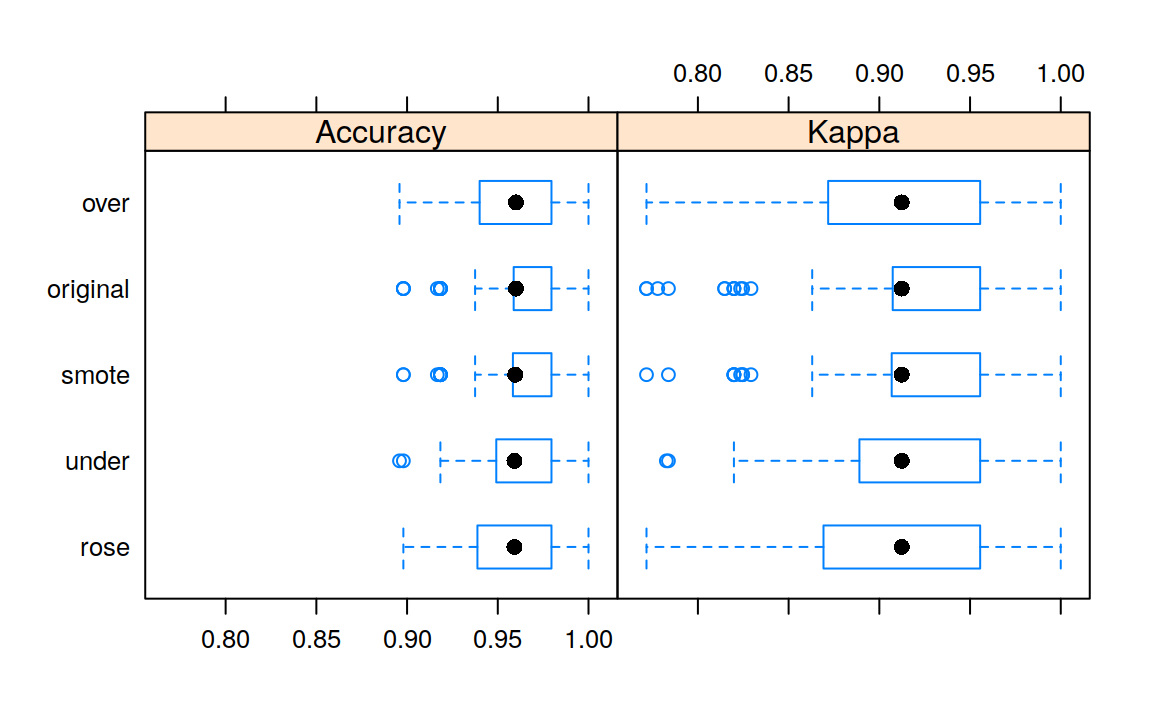
\includegraphics[width=0.7\linewidth]{meta_131-dealing_with_unbalanced_data-sglander_files/figure-latex/plot-resampling-1} \end{center}

\begin{Shaded}
\begin{Highlighting}[]
\KeywordTok{library}\NormalTok{(dplyr)}
\CommentTok{#> }
\CommentTok{#> Attaching package: 'dplyr'}
\CommentTok{#> The following objects are masked from 'package:stats':}
\CommentTok{#> }
\CommentTok{#>     filter, lag}
\CommentTok{#> The following objects are masked from 'package:base':}
\CommentTok{#> }
\CommentTok{#>     intersect, setdiff, setequal, union}
\NormalTok{comparison <-}\StringTok{ }\KeywordTok{data.frame}\NormalTok{(}\DataTypeTok{model =} \KeywordTok{names}\NormalTok{(models),}
                         \DataTypeTok{Sensitivity =} \KeywordTok{rep}\NormalTok{(}\OtherTok{NA}\NormalTok{, }\KeywordTok{length}\NormalTok{(models)),}
                         \DataTypeTok{Specificity =} \KeywordTok{rep}\NormalTok{(}\OtherTok{NA}\NormalTok{, }\KeywordTok{length}\NormalTok{(models)),}
                         \DataTypeTok{Precision   =} \KeywordTok{rep}\NormalTok{(}\OtherTok{NA}\NormalTok{, }\KeywordTok{length}\NormalTok{(models)),}
                         \DataTypeTok{Recall      =} \KeywordTok{rep}\NormalTok{(}\OtherTok{NA}\NormalTok{, }\KeywordTok{length}\NormalTok{(models)),}
                         \DataTypeTok{F1          =} \KeywordTok{rep}\NormalTok{(}\OtherTok{NA}\NormalTok{, }\KeywordTok{length}\NormalTok{(models)))}

\ControlFlowTok{for}\NormalTok{ (name }\ControlFlowTok{in} \KeywordTok{names}\NormalTok{(models)) \{}
\NormalTok{    cm_model <-}\StringTok{ }\KeywordTok{get}\NormalTok{(}\KeywordTok{paste0}\NormalTok{(}\StringTok{"cm_"}\NormalTok{, name))}
\NormalTok{    comparison[comparison}\OperatorTok{$}\NormalTok{model}\OperatorTok{==}\NormalTok{name, ] <-}\StringTok{ }\KeywordTok{filter}\NormalTok{(comparison, model}\OperatorTok{==}\NormalTok{name) }\OperatorTok
\StringTok{    }\KeywordTok{mutate}\NormalTok{(}\DataTypeTok{Sensitivity =}\NormalTok{ cm_model}\OperatorTok{$}\NormalTok{byClass[}\StringTok{"Sensitivity"}\NormalTok{],}
           \DataTypeTok{Specificity =}\NormalTok{ cm_model}\OperatorTok{$}\NormalTok{byClass[}\StringTok{"Specificity"}\NormalTok{],}
           \DataTypeTok{Precision   =}\NormalTok{ cm_model}\OperatorTok{$}\NormalTok{byClass[}\StringTok{"Precision"}\NormalTok{],}
           \DataTypeTok{Recall      =}\NormalTok{ cm_model}\OperatorTok{$}\NormalTok{byClass[}\StringTok{"Recall"}\NormalTok{],}
           \DataTypeTok{F1          =}\NormalTok{ cm_model}\OperatorTok{$}\NormalTok{byClass[}\StringTok{"F1"}\NormalTok{]}
\NormalTok{  )}
\NormalTok{\}    }

\KeywordTok{print}\NormalTok{(comparison)}
\CommentTok{#>      model Sensitivity Specificity Precision Recall    F1}
\CommentTok{#> 1 original       0.978       0.986     0.993  0.978 0.985}
\CommentTok{#> 2    under       0.978       1.000     1.000  0.978 0.989}
\CommentTok{#> 3     over       0.978       0.986     0.993  0.978 0.985}
\CommentTok{#> 4    smote       0.978       0.986     0.993  0.978 0.985}
\CommentTok{#> 5     rose       0.985       0.986     0.993  0.985 0.989}
\end{Highlighting}
\end{Shaded}

\begin{Shaded}
\begin{Highlighting}[]
\KeywordTok{library}\NormalTok{(tidyr)}
\CommentTok{#> }
\CommentTok{#> Attaching package: 'tidyr'}
\CommentTok{#> The following object is masked from 'package:mice':}
\CommentTok{#> }
\CommentTok{#>     complete}
\NormalTok{comparison }\OperatorTok
\StringTok{  }\KeywordTok{gather}\NormalTok{(x, y, Sensitivity}\OperatorTok{:}\NormalTok{F1) }\OperatorTok
\StringTok{  }\KeywordTok{ggplot}\NormalTok{(}\KeywordTok{aes}\NormalTok{(}\DataTypeTok{x =}\NormalTok{ x, }\DataTypeTok{y =}\NormalTok{ y, }\DataTypeTok{color =}\NormalTok{ model)) }\OperatorTok{+}
\StringTok{    }\KeywordTok{geom_jitter}\NormalTok{(}\DataTypeTok{width =} \FloatTok{0.2}\NormalTok{, }\DataTypeTok{alpha =} \FloatTok{0.5}\NormalTok{, }\DataTypeTok{size =} \DecValTok{3}\NormalTok{)}
\end{Highlighting}
\end{Shaded}

\begin{center}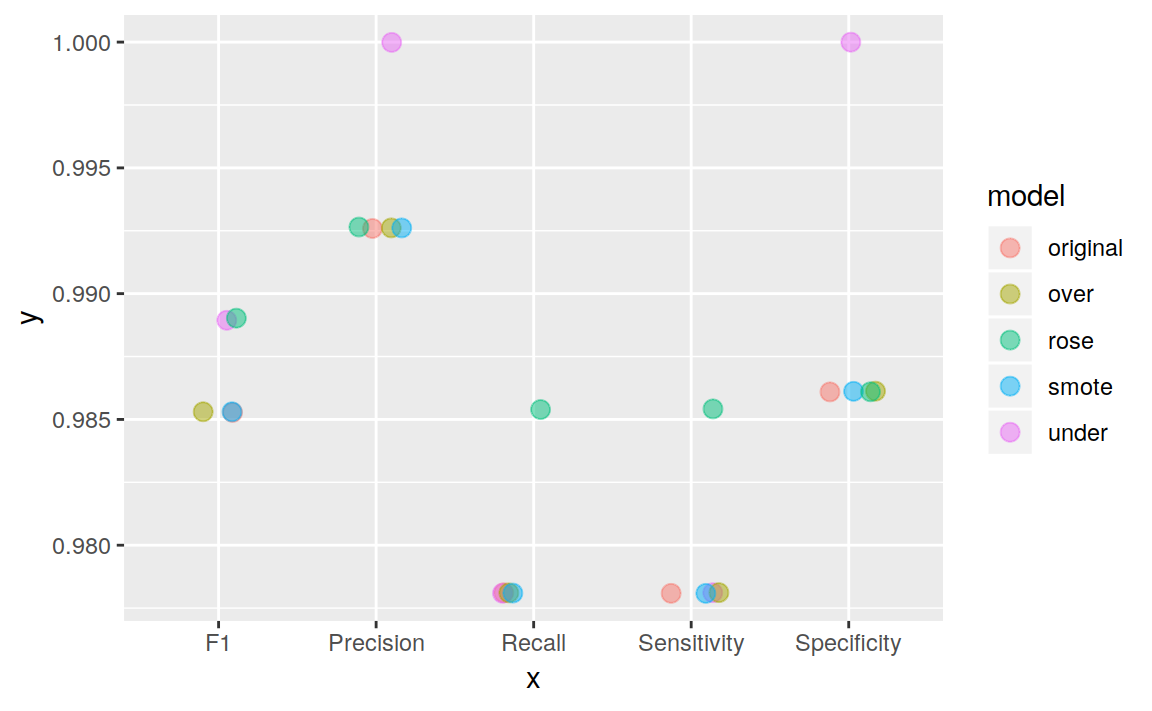
\includegraphics[width=0.7\linewidth]{meta_131-dealing_with_unbalanced_data-sglander_files/figure-latex/comparison-plot-1} \end{center}

With this small dataset, we can already see how the different techniques can influence model performance. \textbf{Sensitivity} (or \textbf{recall}) describes the proportion of benign cases that have been predicted correctly, while \textbf{specificity} describes the proportion of malignant cases that have been predicted correctly. \textbf{Precision describes} the true positives, i.e.~the proportion of benign predictions that were actual from benign samples. \textbf{F1} is the weighted average of precision and sensitivity/ recall.

\hypertarget{final-notes}{%
\section{Final notes}\label{final-notes}}

Here, all four methods improved specificity and precision compared to the original model. Under-sampling, over-sampling and ROSE additionally improved precision and the F1 score.

This post shows a simple example of how to correct for unbalance in datasets for machine learning. For more advanced instructions and potential caveats with these techniques, check out the excellent \texttt{caret} documentation.

If you are interested in more machine learning posts, check out the category listing for machine\_learning on my blog.

\hypertarget{ten-different-methods-to-assess-variable-importance}{%
\chapter{Ten different methods to assess Variable Importance}\label{ten-different-methods-to-assess-variable-importance}}

\hypertarget{glaucoma-dataset}{%
\section{Glaucoma dataset}\label{glaucoma-dataset}}

Source: \url{https://www.machinelearningplus.com/machine-learning/feature-selection/}

\hypertarget{introduction-2}{%
\section{Introduction}\label{introduction-2}}

In real-world datasets, it is fairly common to have columns that are nothing but noise.

You are better off getting rid of such variables because of the memory space they occupy, the time and the computational esources it is going to cost, especially in large datasets.

Sometimes, you have a variable that makes business sense, but you are not sure if it actually helps in predicting the Y. You also need to consider the fact that, a feature that could be useful in one ML algorithm (say a decision tree) may go underrepresented or unused by another (like a regression model).

Having said that, it is still possible that a variable that shows poor signs of helping to explain the response variable (Y), can turn out to be significantly useful in the presence of (or combination with) other predictors. What I mean by that is, a variable might have a low correlation value of (\textasciitilde{}0.2) with Y. But in the presence of other variables, it can help to explain certain patterns/phenomenon that other variables can't explain.

In such cases, it can be hard to make a call whether to include or exclude such variables.

The strategies we are about to discuss can help fix such problems. Not only that, it will also help understand if a particular variable is important or not and how much it is contributing to the model

An important caveat. It is always best to have variables that have sound business logic backing the inclusion of a variable and rely solely on variable importance metrics.

Alright. Let's load up the `Glaucoma' dataset where the goal is to predict if a patient has Glaucoma or not based on 63 different physiological measurements. You can directly run the codes or download the dataset here.

A lot of interesting examples ahead. Let's get started.

\begin{Shaded}
\begin{Highlighting}[]
\CommentTok{# Load Packages and prepare dataset}
\KeywordTok{library}\NormalTok{(TH.data)}
\CommentTok{#> Loading required package: survival}
\CommentTok{#> Loading required package: MASS}
\CommentTok{#> }
\CommentTok{#> Attaching package: 'TH.data'}
\CommentTok{#> The following object is masked from 'package:MASS':}
\CommentTok{#> }
\CommentTok{#>     geyser}
\KeywordTok{library}\NormalTok{(caret)}
\CommentTok{#> Loading required package: lattice}
\CommentTok{#> Loading required package: ggplot2}
\CommentTok{#> Registered S3 methods overwritten by 'ggplot2':}
\CommentTok{#>   method         from }
\CommentTok{#>   [.quosures     rlang}
\CommentTok{#>   c.quosures     rlang}
\CommentTok{#>   print.quosures rlang}
\CommentTok{#> }
\CommentTok{#> Attaching package: 'caret'}
\CommentTok{#> The following object is masked from 'package:survival':}
\CommentTok{#> }
\CommentTok{#>     cluster}
\KeywordTok{library}\NormalTok{(tictoc)}

\KeywordTok{data}\NormalTok{(}\StringTok{"GlaucomaM"}\NormalTok{, }\DataTypeTok{package =} \StringTok{"TH.data"}\NormalTok{)}
\NormalTok{trainData <-}\StringTok{ }\NormalTok{GlaucomaM}
\KeywordTok{head}\NormalTok{(trainData)}
\CommentTok{#>      ag    at    as    an    ai   eag   eat   eas   ean   eai  abrg  abrt}
\CommentTok{#> 2  2.22 0.354 0.580 0.686 0.601 1.267 0.336 0.346 0.255 0.331 0.479 0.260}
\CommentTok{#> 43 2.68 0.475 0.672 0.868 0.667 2.053 0.440 0.520 0.639 0.454 1.090 0.377}
\CommentTok{#> 25 1.98 0.343 0.508 0.624 0.504 1.200 0.299 0.396 0.259 0.246 0.465 0.209}
\CommentTok{#> 65 1.75 0.269 0.476 0.525 0.476 0.612 0.147 0.017 0.044 0.405 0.170 0.062}
\CommentTok{#> 70 2.99 0.599 0.686 1.039 0.667 2.513 0.543 0.607 0.871 0.492 1.800 0.431}
\CommentTok{#> 16 2.92 0.483 0.763 0.901 0.770 2.200 0.462 0.637 0.504 0.597 1.311 0.394}
\CommentTok{#>     abrs  abrn  abri    hic   mhcg  mhct   mhcs   mhcn   mhci   phcg}
\CommentTok{#> 2  0.107 0.014 0.098  0.214  0.111 0.412  0.036  0.105 -0.022 -0.139}
\CommentTok{#> 43 0.257 0.212 0.245  0.382  0.140 0.338  0.104  0.080  0.109 -0.015}
\CommentTok{#> 25 0.112 0.041 0.103  0.195  0.062 0.356  0.045 -0.009 -0.048 -0.149}
\CommentTok{#> 65 0.000 0.000 0.108 -0.030 -0.015 0.074 -0.084 -0.050  0.035 -0.182}
\CommentTok{#> 70 0.494 0.601 0.274  0.383  0.089 0.233  0.145  0.023  0.007 -0.131}
\CommentTok{#> 16 0.365 0.251 0.301  0.442  0.128 0.375  0.049  0.111  0.052 -0.088}
\CommentTok{#>      phct   phcs   phcn   phci   hvc  vbsg  vbst  vbss  vbsn  vbsi  vasg}
\CommentTok{#> 2   0.242 -0.053  0.010 -0.139 0.613 0.303 0.103 0.088 0.022 0.090 0.062}
\CommentTok{#> 43  0.296 -0.015 -0.015  0.036 0.382 0.676 0.181 0.186 0.141 0.169 0.029}
\CommentTok{#> 25  0.206 -0.092 -0.081 -0.149 0.557 0.300 0.084 0.088 0.046 0.082 0.036}
\CommentTok{#> 65 -0.097 -0.125 -0.138 -0.182 0.373 0.048 0.011 0.000 0.000 0.036 0.070}
\CommentTok{#> 70  0.163  0.055 -0.131 -0.115 0.405 0.889 0.151 0.253 0.330 0.155 0.020}
\CommentTok{#> 16  0.281 -0.067 -0.062 -0.088 0.507 0.972 0.213 0.316 0.197 0.246 0.043}
\CommentTok{#>     vast  vass  vasn  vasi  vbrg  vbrt  vbrs  vbrn  vbri  varg  vart  vars}
\CommentTok{#> 2  0.000 0.011 0.032 0.018 0.075 0.039 0.021 0.002 0.014 0.756 0.009 0.209}
\CommentTok{#> 43 0.001 0.007 0.011 0.010 0.370 0.127 0.099 0.050 0.093 0.410 0.006 0.105}
\CommentTok{#> 25 0.002 0.004 0.016 0.013 0.081 0.034 0.019 0.007 0.021 0.565 0.014 0.132}
\CommentTok{#> 65 0.005 0.030 0.033 0.002 0.005 0.001 0.000 0.000 0.004 0.380 0.032 0.147}
\CommentTok{#> 70 0.001 0.004 0.008 0.007 0.532 0.103 0.173 0.181 0.075 0.228 0.011 0.026}
\CommentTok{#> 16 0.001 0.005 0.028 0.009 0.467 0.136 0.148 0.078 0.104 0.540 0.008 0.133}
\CommentTok{#>     varn  vari   mdg   mdt   mds   mdn   mdi    tmg    tmt    tms    tmn}
\CommentTok{#> 2  0.298 0.240 0.705 0.637 0.738 0.596 0.691 -0.236 -0.018 -0.230 -0.510}
\CommentTok{#> 43 0.181 0.117 0.898 0.850 0.907 0.771 0.940 -0.211 -0.014 -0.165 -0.317}
\CommentTok{#> 25 0.243 0.177 0.687 0.643 0.689 0.684 0.700 -0.185 -0.097 -0.235 -0.337}
\CommentTok{#> 65 0.151 0.050 0.207 0.171 0.022 0.046 0.221 -0.148 -0.035 -0.449 -0.217}
\CommentTok{#> 70 0.105 0.087 0.721 0.638 0.730 0.730 0.640 -0.052 -0.105  0.084 -0.012}
\CommentTok{#> 16 0.232 0.167 0.927 0.842 0.953 0.906 0.898 -0.040  0.087  0.018 -0.094}
\CommentTok{#>       tmi    mr   rnf  mdic   emd    mv  Class}
\CommentTok{#> 2  -0.158 0.841 0.410 0.137 0.239 0.035 normal}
\CommentTok{#> 43 -0.192 0.924 0.256 0.252 0.329 0.022 normal}
\CommentTok{#> 25 -0.020 0.795 0.378 0.152 0.250 0.029 normal}
\CommentTok{#> 65 -0.091 0.746 0.200 0.027 0.078 0.023 normal}
\CommentTok{#> 70 -0.054 0.977 0.193 0.297 0.354 0.034 normal}
\CommentTok{#> 16 -0.051 0.965 0.339 0.333 0.442 0.028 normal}
\end{Highlighting}
\end{Shaded}

\hypertarget{boruta}{%
\section{1. Boruta}\label{boruta}}

Boruta is a feature ranking and selection algorithm based on random forests algorithm.

The advantage with Boruta is that it clearly decides if a variable is important or not and helps to select variables that are statistically significant. Besides, you can adjust the strictness of the algorithm by adjusting the \(p\) values that defaults to 0.01 and the \texttt{maxRuns}.

\texttt{maxRuns} is the number of times the algorithm is run. The higher the \texttt{maxRuns} the more selective you get in picking the variables. The default value is 100.

In the process of deciding if a feature is important or not, some features may be marked by Boruta as `Tentative'. Sometimes increasing the maxRuns can help resolve the `Tentativeness' of the feature.

Lets see an example based on the Glaucoma dataset from \texttt{TH.data} package that I created earlier.

\begin{Shaded}
\begin{Highlighting}[]
\CommentTok{# install.packages('Boruta')}
\KeywordTok{library}\NormalTok{(Boruta)}
\CommentTok{#> Loading required package: ranger}
\end{Highlighting}
\end{Shaded}

The \texttt{boruta} function uses a formula interface just like most predictive modeling functions. So the first argument to \texttt{boruta()} is the formula with the response variable on the left and all the predictors on the right.

By placing a dot, all the variables in \texttt{trainData} other than Class will be included in the model.

The \texttt{doTrace} argument controls the amount of output printed to the console. Higher the value, more the log details you get. So save space I have set it to 0, but try setting it to 1 and 2 if you are running the code.

Finally the output is stored in \texttt{boruta\_output}.

\begin{Shaded}
\begin{Highlighting}[]
\CommentTok{# Perform Boruta search}
\NormalTok{boruta_output <-}\StringTok{ }\KeywordTok{Boruta}\NormalTok{(Class }\OperatorTok{~}\StringTok{ }\NormalTok{., }\DataTypeTok{data=}\KeywordTok{na.omit}\NormalTok{(trainData), }\DataTypeTok{doTrace=}\DecValTok{0}\NormalTok{)  }
\end{Highlighting}
\end{Shaded}

Let's see what the boruta\_output contains.

\begin{Shaded}
\begin{Highlighting}[]
\KeywordTok{names}\NormalTok{(boruta_output)}
\CommentTok{#>  [1] "finalDecision" "ImpHistory"    "pValue"        "maxRuns"      }
\CommentTok{#>  [5] "light"         "mcAdj"         "timeTaken"     "roughfixed"   }
\CommentTok{#>  [9] "call"          "impSource"}
\end{Highlighting}
\end{Shaded}

\begin{Shaded}
\begin{Highlighting}[]
\CommentTok{# Get significant variables including tentatives}
\NormalTok{boruta_signif <-}\StringTok{ }\KeywordTok{getSelectedAttributes}\NormalTok{(boruta_output, }\DataTypeTok{withTentative =} \OtherTok{TRUE}\NormalTok{)}
\KeywordTok{print}\NormalTok{(boruta_signif)  }
\CommentTok{#>  [1] "as"   "ai"   "eas"  "ean"  "abrg" "abrs" "abrn" "abri" "hic"  "mhcg"}
\CommentTok{#> [11] "mhcs" "mhcn" "mhci" "phcg" "phcn" "phci" "hvc"  "vbsg" "vbss" "vbsn"}
\CommentTok{#> [21] "vbsi" "vasg" "vass" "vasi" "vbrg" "vbrs" "vbrn" "vbri" "varg" "vart"}
\CommentTok{#> [31] "vars" "varn" "vari" "mdn"  "tmg"  "tmt"  "tms"  "tmi"  "mr"   "rnf" }
\CommentTok{#> [41] "mdic" "emd"}
\end{Highlighting}
\end{Shaded}

If you are not sure about the tentative variables being selected for granted, you can choose a \texttt{TentativeRoughFix} on \texttt{boruta\_output}.

\begin{Shaded}
\begin{Highlighting}[]
\CommentTok{# Do a tentative rough fix}
\NormalTok{roughFixMod <-}\StringTok{ }\KeywordTok{TentativeRoughFix}\NormalTok{(boruta_output)}
\NormalTok{boruta_signif <-}\StringTok{ }\KeywordTok{getSelectedAttributes}\NormalTok{(roughFixMod)}
\KeywordTok{print}\NormalTok{(boruta_signif)}
\CommentTok{#>  [1] "as"   "ai"   "ean"  "abrg" "abrs" "abrn" "abri" "hic"  "mhcg" "mhcn"}
\CommentTok{#> [11] "mhci" "phcg" "phcn" "phci" "hvc"  "vbsn" "vbsi" "vasg" "vass" "vasi"}
\CommentTok{#> [21] "vbrg" "vbrs" "vbrn" "vbri" "varg" "vart" "vars" "varn" "vari" "mdn" }
\CommentTok{#> [31] "tmg"  "tms"  "tmi"  "mr"   "rnf"  "mdic"}
\end{Highlighting}
\end{Shaded}

There you go. Boruta has decided on the `Tentative' variables on our behalf. Let's find out the importance scores of these variables.

\begin{Shaded}
\begin{Highlighting}[]
\CommentTok{# Variable Importance Scores}
\NormalTok{imps <-}\StringTok{ }\KeywordTok{attStats}\NormalTok{(roughFixMod)}
\NormalTok{imps2 =}\StringTok{ }\NormalTok{imps[imps}\OperatorTok{$}\NormalTok{decision }\OperatorTok{!=}\StringTok{ 'Rejected'}\NormalTok{, }\KeywordTok{c}\NormalTok{(}\StringTok{'meanImp'}\NormalTok{, }\StringTok{'decision'}\NormalTok{)]}
\KeywordTok{head}\NormalTok{(imps2[}\KeywordTok{order}\NormalTok{(}\OperatorTok{-}\NormalTok{imps2}\OperatorTok{$}\NormalTok{meanImp), ])  }\CommentTok{# descending sort}
\CommentTok{#>      meanImp  decision}
\CommentTok{#> vari   12.37 Confirmed}
\CommentTok{#> varg   11.74 Confirmed}
\CommentTok{#> vars   10.74 Confirmed}
\CommentTok{#> phci    8.34 Confirmed}
\CommentTok{#> hic     8.21 Confirmed}
\CommentTok{#> varn    7.88 Confirmed}
\end{Highlighting}
\end{Shaded}

Let's plot it to see the importances of these variables.

\begin{Shaded}
\begin{Highlighting}[]
\CommentTok{# Plot variable importance}
\KeywordTok{plot}\NormalTok{(boruta_output, }\DataTypeTok{cex.axis=}\NormalTok{.}\DecValTok{7}\NormalTok{, }\DataTypeTok{las=}\DecValTok{2}\NormalTok{, }\DataTypeTok{xlab=}\StringTok{""}\NormalTok{, }\DataTypeTok{main=}\StringTok{"Variable Importance"}\NormalTok{)  }
\end{Highlighting}
\end{Shaded}

\begin{center}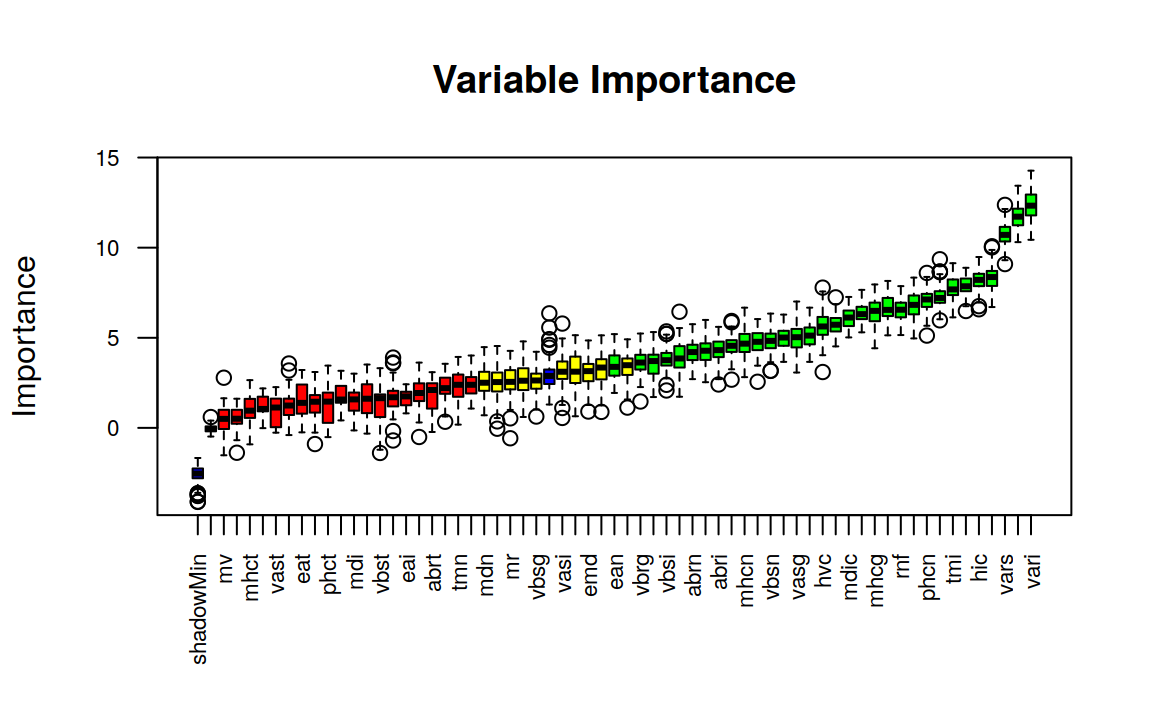
\includegraphics[width=0.7\linewidth]{meta_133-variable_importance_files/figure-latex/boruta-plot-1} \end{center}

This plot reveals the importance of each of the features.

The columns in green are `confirmed' and the ones in red are not. There are couple of blue bars representing \texttt{ShadowMax} and \texttt{ShadowMin.} They are not actual features, but are used by the boruta algorithm to decide if a variable is important or not.

\hypertarget{variable-importance-from-machine-learning-algorithms}{%
\section{Variable Importance from Machine Learning Algorithms}\label{variable-importance-from-machine-learning-algorithms}}

Another way to look at feature selection is to consider variables most used by various ML algorithms the most to be important.

Depending on how the machine learning algorithm learns the relationship between X's and Y, different machine learning algorithms may possibly end up using different variables (but mostly common vars) to various degrees.

What I mean by that is, the variables that proved useful in a tree-based algorithm like \texttt{rpart}, can turn out to be less useful in a regression-based model. So all variables need not be equally useful to all algorithms.

So how do we find the variable importance for a given ML algo?

\texttt{train()} the desired model using the caret package.
Then, use \texttt{varImp()} to determine the feature importances.

You may want to try out multiple algorithms, to get a feel of the usefulness of the features across algos.

\hypertarget{rpart}{%
\subsection{rpart}\label{rpart}}

\begin{Shaded}
\begin{Highlighting}[]
\CommentTok{# Train an rpart model and compute variable importance.}
\KeywordTok{library}\NormalTok{(caret)}
\KeywordTok{set.seed}\NormalTok{(}\DecValTok{100}\NormalTok{)}
\NormalTok{rPartMod <-}\StringTok{ }\KeywordTok{train}\NormalTok{(Class }\OperatorTok{~}\StringTok{ }\NormalTok{., }
                  \DataTypeTok{data=}\NormalTok{trainData, }
                  \DataTypeTok{method=}\StringTok{"rpart"}\NormalTok{)}

\NormalTok{rpartImp <-}\StringTok{ }\KeywordTok{varImp}\NormalTok{(rPartMod)}
\KeywordTok{print}\NormalTok{(rpartImp)}
\CommentTok{#> rpart variable importance}
\CommentTok{#> }
\CommentTok{#>   only 20 most important variables shown (out of 62)}
\CommentTok{#> }
\CommentTok{#>      Overall}
\CommentTok{#> varg   100.0}
\CommentTok{#> vari    93.2}
\CommentTok{#> vars    85.2}
\CommentTok{#> varn    76.9}
\CommentTok{#> tmi     72.3}
\CommentTok{#> mhcn     0.0}
\CommentTok{#> as       0.0}
\CommentTok{#> phcs     0.0}
\CommentTok{#> vbst     0.0}
\CommentTok{#> abrt     0.0}
\CommentTok{#> vbsg     0.0}
\CommentTok{#> eai      0.0}
\CommentTok{#> vbrs     0.0}
\CommentTok{#> vbsi     0.0}
\CommentTok{#> eag      0.0}
\CommentTok{#> tmt      0.0}
\CommentTok{#> phcn     0.0}
\CommentTok{#> vart     0.0}
\CommentTok{#> mds      0.0}
\CommentTok{#> an       0.0}
\end{Highlighting}
\end{Shaded}

Only 5 of the 63 features was used by rpart and if you look closely, the 5 variables used here are in the top 6 that boruta selected.

Let's do one more: the variable importances from Regularized Random Forest (RRF) algorithm.

\hypertarget{regularized-random-forest-rrf}{%
\subsection{Regularized Random Forest (RRF)}\label{regularized-random-forest-rrf}}

\begin{Shaded}
\begin{Highlighting}[]
\KeywordTok{tic}\NormalTok{()}
\CommentTok{# Train an RRF model and compute variable importance.}
\KeywordTok{set.seed}\NormalTok{(}\DecValTok{100}\NormalTok{)}
\NormalTok{rrfMod <-}\StringTok{ }\KeywordTok{train}\NormalTok{(Class }\OperatorTok{~}\StringTok{ }\NormalTok{., }
                \DataTypeTok{data =}\NormalTok{ trainData, }
                \DataTypeTok{method =} \StringTok{"RRF"}\NormalTok{)}
\CommentTok{#> Registered S3 method overwritten by 'RRF':}
\CommentTok{#>   method      from        }
\CommentTok{#>   plot.margin randomForest}

\NormalTok{rrfImp <-}\StringTok{ }\KeywordTok{varImp}\NormalTok{(rrfMod, }\DataTypeTok{scale=}\NormalTok{F)}
\KeywordTok{toc}\NormalTok{()}
\CommentTok{#> 345.177 sec elapsed}
\NormalTok{rrfImp}
\CommentTok{#> RRF variable importance}
\CommentTok{#> }
\CommentTok{#>   only 20 most important variables shown (out of 62)}
\CommentTok{#> }
\CommentTok{#>      Overall}
\CommentTok{#> varg   25.07}
\CommentTok{#> vari   18.78}
\CommentTok{#> vars    5.29}
\CommentTok{#> tmi     4.09}
\CommentTok{#> mhcg    3.25}
\CommentTok{#> mhci    2.81}
\CommentTok{#> hic     2.69}
\CommentTok{#> hvc     2.50}
\CommentTok{#> mv      2.00}
\CommentTok{#> vasg    1.99}
\CommentTok{#> phci    1.77}
\CommentTok{#> phcn    1.53}
\CommentTok{#> phct    1.43}
\CommentTok{#> vass    1.37}
\CommentTok{#> phcg    1.37}
\CommentTok{#> tms     1.32}
\CommentTok{#> tmg     1.16}
\CommentTok{#> abrs    1.16}
\CommentTok{#> tmt     1.13}
\CommentTok{#> mdic    1.13}
\end{Highlighting}
\end{Shaded}

\begin{Shaded}
\begin{Highlighting}[]
\KeywordTok{plot}\NormalTok{(rrfImp, }\DataTypeTok{top =} \DecValTok{20}\NormalTok{, }\DataTypeTok{main=}\StringTok{'Variable Importance'}\NormalTok{)}
\end{Highlighting}
\end{Shaded}

\begin{center}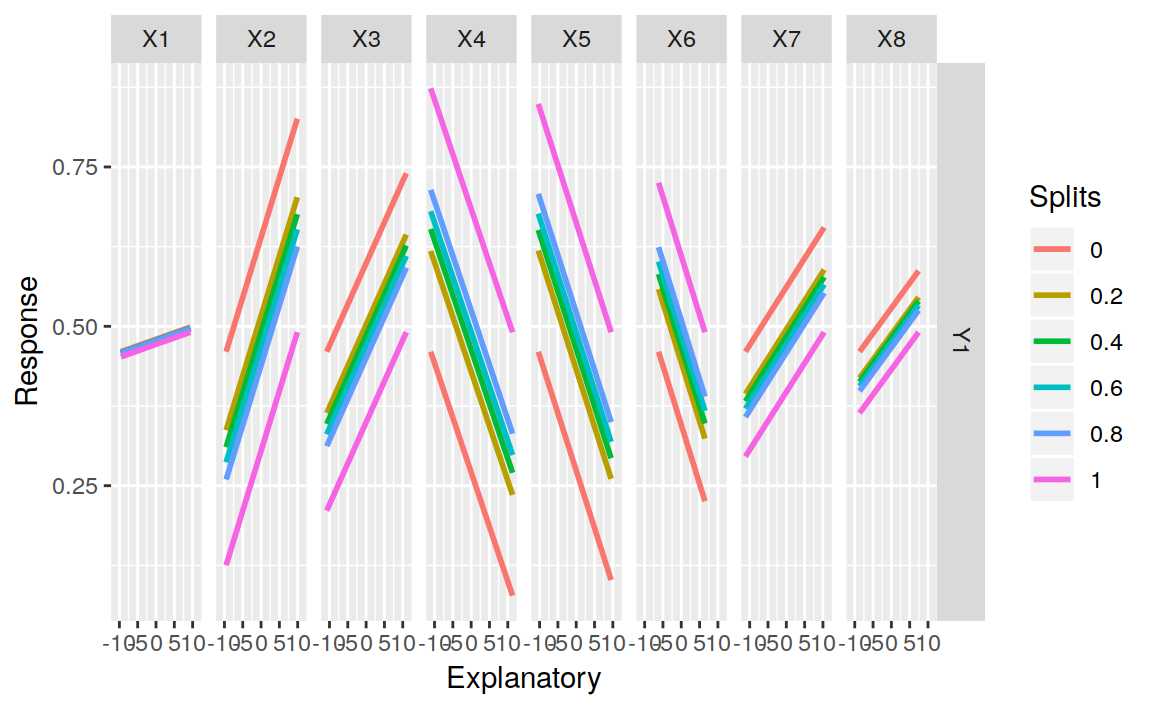
\includegraphics[width=0.7\linewidth]{meta_133-variable_importance_files/figure-latex/unnamed-chunk-9-1} \end{center}

The topmost important variables are pretty much from the top tier of Boruta's selections.

Some of the other algorithms available in \texttt{train()} that you can use to compute varImp are the following:

\begin{verbatim}
ada, AdaBag, AdaBoost.M1, adaboost, bagEarth, bagEarthGCV, bagFDA, bagFDAGCV, bartMachine, blasso, BstLm, bstSm, C5.0, C5.0Cost, C5.0Rules, C5.0Tree, cforest, chaid, ctree, ctree2, cubist, deepboost, earth, enet, evtree, extraTrees, fda, gamboost, gbm_h2o, gbm, gcvEarth, glmnet_h2o, glmnet, glmStepAIC, J48, JRip, lars, lars2, lasso, LMT, LogitBoost, M5, M5Rules, msaenet, nodeHarvest, OneR, ordinalNet, ORFlog, ORFpls, ORFridge, ORFsvm, pam, parRF, PART, penalized, PenalizedLDA, qrf, ranger, Rborist, relaxo, rf, rFerns, rfRules, rotationForest, rotationForestCp, rpart, rpart1SE, rpart2, rpartCost, rpartScore, rqlasso, rqnc, RRF, RRFglobal, sdwd, smda, sparseLDA, spikeslab, wsrf, xgbLinear, xgbTree.
\end{verbatim}

\hypertarget{lasso-regression}{%
\section{Lasso Regression}\label{lasso-regression}}

Least Absolute Shrinkage and Selection Operator (LASSO) regression is a type of regularization method that penalizes with L1-norm.

It basically imposes a cost to having large weights (value of coefficients). And its called L1 regularization, because the cost added, is proportional to the absolute value of weight coefficients.

As a result, in the process of shrinking the coefficients, it eventually reduces the coefficients of certain unwanted features all the to zero. That is, it removes the unneeded variables altogether.

So effectively, LASSO regression can be considered as a variable selection technique as well.

\begin{Shaded}
\begin{Highlighting}[]
\KeywordTok{library}\NormalTok{(glmnet)}
\CommentTok{#> Loading required package: Matrix}
\CommentTok{#> Loading required package: foreach}
\CommentTok{#> Loaded glmnet 2.0-16}

\CommentTok{# online data}
\CommentTok{# trainData <- read.csv('https://raw.githubusercontent.com/selva86/datasets/master/GlaucomaM.csv')}

\NormalTok{trainData <-}\StringTok{ }\KeywordTok{read.csv}\NormalTok{(}\KeywordTok{file.path}\NormalTok{(data_raw_dir, }\StringTok{"glaucoma.csv"}\NormalTok{))}

\NormalTok{x <-}\StringTok{ }\KeywordTok{as.matrix}\NormalTok{(trainData[,}\OperatorTok{-}\DecValTok{63}\NormalTok{]) }\CommentTok{# all X vars}
\NormalTok{y <-}\StringTok{ }\KeywordTok{as.double}\NormalTok{(}\KeywordTok{as.matrix}\NormalTok{(}\KeywordTok{ifelse}\NormalTok{(trainData[, }\DecValTok{63}\NormalTok{]}\OperatorTok{==}\StringTok{'normal'}\NormalTok{, }\DecValTok{0}\NormalTok{, }\DecValTok{1}\NormalTok{))) }\CommentTok{# Only Class}

\CommentTok{# Fit the LASSO model (Lasso: Alpha = 1)}
\KeywordTok{set.seed}\NormalTok{(}\DecValTok{100}\NormalTok{)}
\NormalTok{cv.lasso <-}\StringTok{ }\KeywordTok{cv.glmnet}\NormalTok{(x, y, }\DataTypeTok{family=}\StringTok{'binomial'}\NormalTok{, }\DataTypeTok{alpha=}\DecValTok{1}\NormalTok{, }\DataTypeTok{parallel=}\OtherTok{TRUE}\NormalTok{, }\DataTypeTok{standardize=}\OtherTok{TRUE}\NormalTok{, }\DataTypeTok{type.measure=}\StringTok{'auc'}\NormalTok{)}
\CommentTok{#> Warning: executing %dopar% sequentially: no parallel backend registered}

\CommentTok{# Results}
\KeywordTok{plot}\NormalTok{(cv.lasso)}
\end{Highlighting}
\end{Shaded}

\begin{center}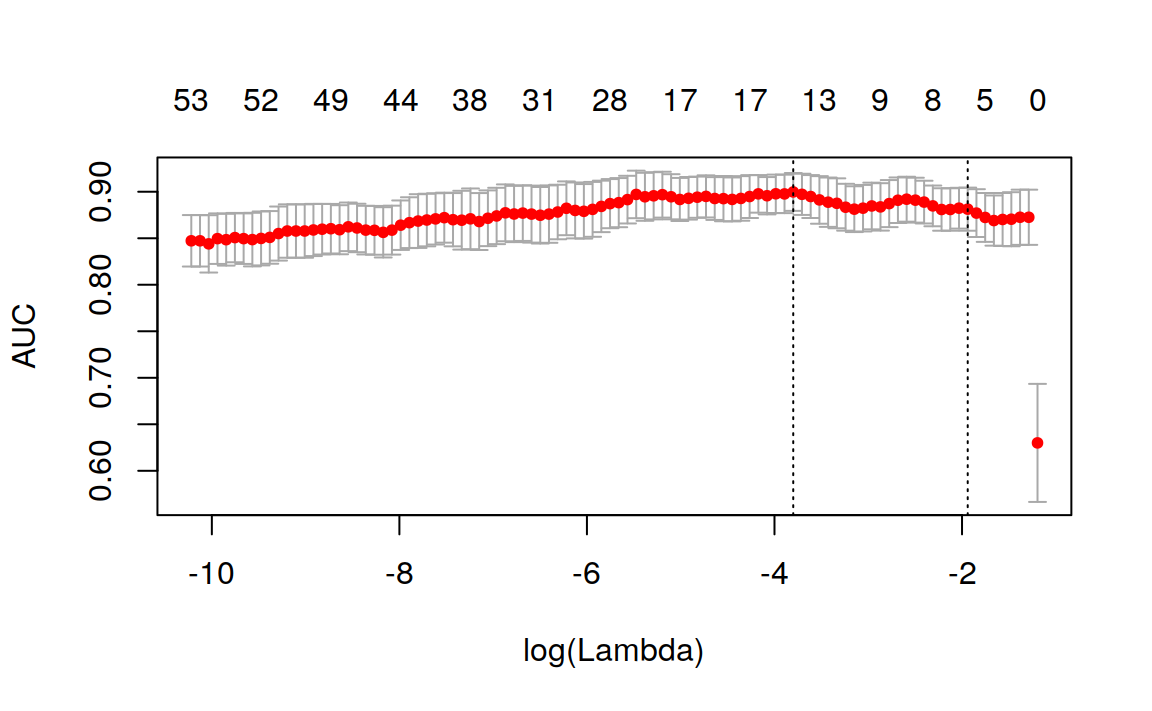
\includegraphics[width=0.7\linewidth]{meta_133-variable_importance_files/figure-latex/lasso-train-1} \end{center}

Let's see how to interpret this plot.

The X axis of the plot is the log of \texttt{lambda}. That means when it is 2 here, the lambda value is actually 100.

The numbers at the top of the plot show how many predictors were included in the model. The position of red dots along the Y-axis tells what \texttt{AUC} we got when you include as many variables shown on the top x-axis.

You can also see two dashed vertical lines.

The first one on the left points to the lambda with the lowest mean squared error. The one on the right point to the number of variables with the highest deviance within 1 standard deviation.

The best lambda value is stored inside `cv.lasso\$lambda.min'.

\begin{Shaded}
\begin{Highlighting}[]
\CommentTok{# plot(cv.lasso$glmnet.fit, xvar="lambda", label=TRUE)}
\KeywordTok{cat}\NormalTok{(}\StringTok{'Min Lambda: '}\NormalTok{, cv.lasso}\OperatorTok{$}\NormalTok{lambda.min, }\StringTok{'}\CharTok{\textbackslash{}n}\StringTok{ 1Sd Lambda: '}\NormalTok{, cv.lasso}\OperatorTok{$}\NormalTok{lambda}\FloatTok{.1}\NormalTok{se)}
\CommentTok{#> Min Lambda:  0.0224 }
\CommentTok{#>  1Sd Lambda:  0.144}
\NormalTok{df_coef <-}\StringTok{ }\KeywordTok{round}\NormalTok{(}\KeywordTok{as.matrix}\NormalTok{(}\KeywordTok{coef}\NormalTok{(cv.lasso, }\DataTypeTok{s=}\NormalTok{cv.lasso}\OperatorTok{$}\NormalTok{lambda.min)), }\DecValTok{2}\NormalTok{)}

\CommentTok{# See all contributing variables}
\NormalTok{df_coef[df_coef[, }\DecValTok{1}\NormalTok{] }\OperatorTok{!=}\StringTok{ }\DecValTok{0}\NormalTok{, ]}
\CommentTok{#> (Intercept)          as        mhci        phci         hvc        vast }
\CommentTok{#>        2.68       -1.59        3.85        5.60       -2.41      -13.90 }
\CommentTok{#>        vars        vari         mdn         mdi         tmg         tms }
\CommentTok{#>      -20.18       -1.58        0.50        0.99        0.06        2.56 }
\CommentTok{#>         tmi }
\CommentTok{#>        2.23}
\end{Highlighting}
\end{Shaded}

The above output shows what variables LASSO considered important. A high positive or low negative implies more important is that variable.

\hypertarget{step-wise-forward-and-backward-selection}{%
\section{Step wise Forward and Backward Selection}\label{step-wise-forward-and-backward-selection}}

Stepwise regression can be used to select features if the Y variable is a numeric variable. It is particularly used in selecting best linear regression models.

It searches for the best possible regression model by iteratively selecting and dropping variables to arrive at a model with the lowest possible AIC.

It can be implemented using the \texttt{step()} function and you need to provide it with a lower model, which is the base model from which it won't remove any features and an upper model, which is a full model that has all possible features you want to have.

Our case is not so complicated (\textless{} 20 vars), so lets just do a simple stepwise in `both' directions.

I will use the \texttt{ozone} dataset for this where the objective is to predict the \texttt{ozone\_reading} based on other weather related observations.

\begin{Shaded}
\begin{Highlighting}[]
\CommentTok{# Load data}
\CommentTok{# online}
\CommentTok{# trainData <- read.csv("http://rstatistics.net/wp-content/uploads/2015/09/ozone1.csv",}
\CommentTok{#                      stringsAsFactors=F)}
\NormalTok{trainData <-}\StringTok{ }\KeywordTok{read.csv}\NormalTok{(}\KeywordTok{file.path}\NormalTok{(data_raw_dir, }\StringTok{"ozone1.csv"}\NormalTok{))}
\KeywordTok{print}\NormalTok{(}\KeywordTok{head}\NormalTok{(trainData))}
\CommentTok{#>   Month Day_of_month Day_of_week ozone_reading pressure_height Wind_speed}
\CommentTok{#> 1     1            1           4             3            5480          8}
\CommentTok{#> 2     1            2           5             3            5660          6}
\CommentTok{#> 3     1            3           6             3            5710          4}
\CommentTok{#> 4     1            4           7             5            5700          3}
\CommentTok{#> 5     1            5           1             5            5760          3}
\CommentTok{#> 6     1            6           2             6            5720          4}
\CommentTok{#>   Humidity Temperature_Sandburg Temperature_ElMonte Inversion_base_height}
\CommentTok{#> 1       20                 40.5                39.8                  5000}
\CommentTok{#> 2       41                 38.0                46.7                  4109}
\CommentTok{#> 3       28                 40.0                49.5                  2693}
\CommentTok{#> 4       37                 45.0                52.3                   590}
\CommentTok{#> 5       51                 54.0                45.3                  1450}
\CommentTok{#> 6       69                 35.0                49.6                  1568}
\CommentTok{#>   Pressure_gradient Inversion_temperature Visibility}
\CommentTok{#> 1               -15                  30.6        200}
\CommentTok{#> 2               -14                  48.0        300}
\CommentTok{#> 3               -25                  47.7        250}
\CommentTok{#> 4               -24                  55.0        100}
\CommentTok{#> 5                25                  57.0         60}
\CommentTok{#> 6                15                  53.8         60}
\end{Highlighting}
\end{Shaded}

The data is ready. Let's perform the stepwise.

\begin{Shaded}
\begin{Highlighting}[]
\CommentTok{# Step 1: Define base intercept only model}
\NormalTok{base.mod <-}\StringTok{ }\KeywordTok{lm}\NormalTok{(ozone_reading }\OperatorTok{~}\StringTok{ }\DecValTok{1}\NormalTok{ , }\DataTypeTok{data=}\NormalTok{trainData)  }

\CommentTok{# Step 2: Full model with all predictors}
\NormalTok{all.mod <-}\StringTok{ }\KeywordTok{lm}\NormalTok{(ozone_reading }\OperatorTok{~}\StringTok{ }\NormalTok{. , }\DataTypeTok{data=}\NormalTok{ trainData) }

\CommentTok{# Step 3: Perform step-wise algorithm. direction='both' implies both forward and backward stepwise}
\NormalTok{stepMod <-}\StringTok{ }\KeywordTok{step}\NormalTok{(base.mod, }\DataTypeTok{scope =} \KeywordTok{list}\NormalTok{(}\DataTypeTok{lower =}\NormalTok{ base.mod, }\DataTypeTok{upper =}\NormalTok{ all.mod), }\DataTypeTok{direction =} \StringTok{"both"}\NormalTok{, }\DataTypeTok{trace =} \DecValTok{0}\NormalTok{, }\DataTypeTok{steps =} \DecValTok{1000}\NormalTok{)  }

\CommentTok{# Step 4: Get the shortlisted variable.}
\NormalTok{shortlistedVars <-}\StringTok{ }\KeywordTok{names}\NormalTok{(}\KeywordTok{unlist}\NormalTok{(stepMod[[}\DecValTok{1}\NormalTok{]])) }
\NormalTok{shortlistedVars <-}\StringTok{ }\NormalTok{shortlistedVars[}\OperatorTok{!}\NormalTok{shortlistedVars }\OperatorTok\StringTok{ "(Intercept)"}\NormalTok{] }\CommentTok{# remove intercept}

\CommentTok{# Show}
\KeywordTok{print}\NormalTok{(shortlistedVars)}
\CommentTok{#> [1] "Temperature_Sandburg"  "Humidity"              "Temperature_ElMonte"  }
\CommentTok{#> [4] "Month"                 "pressure_height"       "Inversion_base_height"}
\end{Highlighting}
\end{Shaded}

The selected model has the above 6 features in it.

But if you have too many features (\textgreater{} 100) in training data, then it might be a good idea to split the dataset into chunks of 10 variables each with Y as mandatory in each dataset. Loop through all the chunks and collect the best features.

We are doing it this way because some variables that came as important in a training data with fewer features may not show up in a linear reg model built on lots of features.

Finally, from a pool of shortlisted features (from small chunk models), run a full stepwise model to get the final set of selected features.

You can take this as a learning assignment to be solved within 20 minutes.

\hypertarget{relative-importance-from-linear-regression}{%
\section{Relative Importance from Linear Regression}\label{relative-importance-from-linear-regression}}

This technique is specific to linear regression models.

Relative importance can be used to assess which variables contributed how much in explaining the linear model's R-squared value. So, if you sum up the produced importances, it will add up to the model's R-sq value.

In essence, it is not directly a feature selection method, because you have already provided the features that go in the model. But after building the model, the \texttt{relaimpo} can provide a sense of how important each feature is in contributing to the R-sq, or in other words, in `explaining the Y variable'.

So, how to calculate relative importance?

It is implemented in the \texttt{relaimpo} package. Basically, you build a linear regression model and pass that as the main argument to \texttt{calc.relimp()}. relaimpo has multiple options to compute the relative importance, but the recommended method is to use \texttt{type=\textquotesingle{}lmg\textquotesingle{}}, as I have done below.

\begin{Shaded}
\begin{Highlighting}[]
\CommentTok{# install.packages('relaimpo')}
\KeywordTok{library}\NormalTok{(relaimpo)}
\CommentTok{#> Loading required package: boot}
\CommentTok{#> }
\CommentTok{#> Attaching package: 'boot'}
\CommentTok{#> The following object is masked from 'package:lattice':}
\CommentTok{#> }
\CommentTok{#>     melanoma}
\CommentTok{#> The following object is masked from 'package:survival':}
\CommentTok{#> }
\CommentTok{#>     aml}
\CommentTok{#> Loading required package: survey}
\CommentTok{#> Loading required package: grid}
\CommentTok{#> }
\CommentTok{#> Attaching package: 'survey'}
\CommentTok{#> The following object is masked from 'package:graphics':}
\CommentTok{#> }
\CommentTok{#>     dotchart}
\CommentTok{#> Loading required package: mitools}
\CommentTok{#> This is the global version of package relaimpo.}
\CommentTok{#> If you are a non-US user, a version with the interesting additional metric pmvd is available}
\CommentTok{#> from Ulrike Groempings web site at prof.beuth-hochschule.de/groemping.}

\CommentTok{# Build linear regression model}
\NormalTok{model_formula =}\StringTok{ }\NormalTok{ozone_reading }\OperatorTok{~}\StringTok{ }\NormalTok{Temperature_Sandburg }\OperatorTok{+}\StringTok{ }\NormalTok{Humidity }\OperatorTok{+}\StringTok{ }\NormalTok{Temperature_ElMonte }\OperatorTok{+}\StringTok{ }\NormalTok{Month }\OperatorTok{+}\StringTok{ }\NormalTok{pressure_height }\OperatorTok{+}\StringTok{ }\NormalTok{Inversion_base_height}
\NormalTok{lmMod <-}\StringTok{ }\KeywordTok{lm}\NormalTok{(model_formula, }\DataTypeTok{data=}\NormalTok{trainData)}

\CommentTok{# calculate relative importance}
\NormalTok{relImportance <-}\StringTok{ }\KeywordTok{calc.relimp}\NormalTok{(lmMod, }\DataTypeTok{type =} \StringTok{"lmg"}\NormalTok{, }\DataTypeTok{rela =}\NormalTok{ F)  }

\CommentTok{# Sort}
\KeywordTok{cat}\NormalTok{(}\StringTok{'Relative Importances: }\CharTok{\textbackslash{}n}\StringTok{'}\NormalTok{)}
\CommentTok{#> Relative Importances:}
\KeywordTok{sort}\NormalTok{(}\KeywordTok{round}\NormalTok{(relImportance}\OperatorTok{$}\NormalTok{lmg, }\DecValTok{3}\NormalTok{), }\DataTypeTok{decreasing=}\OtherTok{TRUE}\NormalTok{)}
\CommentTok{#>   Temperature_ElMonte  Temperature_Sandburg       pressure_height }
\CommentTok{#>                 0.214                 0.203                 0.104 }
\CommentTok{#> Inversion_base_height              Humidity                 Month }
\CommentTok{#>                 0.096                 0.086                 0.012}
\end{Highlighting}
\end{Shaded}

Additionally, you can use bootstrapping (using \texttt{boot.relimp}) to compute the confidence intervals of the produced relative importances.

\begin{Shaded}
\begin{Highlighting}[]
\NormalTok{bootsub <-}\StringTok{ }\KeywordTok{boot.relimp}\NormalTok{(ozone_reading }\OperatorTok{~}\StringTok{ }\NormalTok{Temperature_Sandburg }\OperatorTok{+}\StringTok{ }\NormalTok{Humidity }\OperatorTok{+}\StringTok{ }\NormalTok{Temperature_ElMonte }\OperatorTok{+}\StringTok{ }\NormalTok{Month }\OperatorTok{+}\StringTok{ }\NormalTok{pressure_height }\OperatorTok{+}\StringTok{ }\NormalTok{Inversion_base_height, }\DataTypeTok{data=}\NormalTok{trainData,}
                       \DataTypeTok{b =} \DecValTok{1000}\NormalTok{, }\DataTypeTok{type =} \StringTok{'lmg'}\NormalTok{, }\DataTypeTok{rank =} \OtherTok{TRUE}\NormalTok{, }\DataTypeTok{diff =} \OtherTok{TRUE}\NormalTok{)}

\KeywordTok{plot}\NormalTok{(}\KeywordTok{booteval.relimp}\NormalTok{(bootsub, }\DataTypeTok{level=}\NormalTok{.}\DecValTok{95}\NormalTok{))}
\end{Highlighting}
\end{Shaded}

\begin{center}\includegraphics[width=0.7\linewidth]{meta_133-variable_importance_files/figure-latex/unnamed-chunk-11-1} \end{center}

\hypertarget{recursive-feature-elimination-rfe}{%
\section{Recursive Feature Elimination (RFE)}\label{recursive-feature-elimination-rfe}}

Recursive feature elimnation (rfe) offers a rigorous way to determine the important variables before you even feed them into a ML algo.

It can be implemented using the \texttt{rfe()} from caret package.

The rfe() also takes two important parameters.

\begin{itemize}
\tightlist
\item
  \texttt{sizes}
\item
  \texttt{rfeControl}
\end{itemize}

So, what does \texttt{sizes} and \texttt{rfeControl} represent?

The sizes determines the number of most important features the rfe should iterate. Below, I have set the size as 1 to 5, 10, 15 and 18.

Secondly, the \texttt{rfeControl} parameter receives the output of the \texttt{rfeControl()}. You can set what type of variable evaluation algorithm must be used. Here, I have used random forests based rfFuncs. The \texttt{method=\textquotesingle{}repeatedCV\textquotesingle{}} means it will do a repeated k-Fold cross validation with \texttt{repeats=5}.

Once complete, you get the accuracy and kappa for each model size you provided. The final selected model subset size is marked with a * in the rightmost selected column.

\begin{Shaded}
\begin{Highlighting}[]
\KeywordTok{str}\NormalTok{(trainData)}
\CommentTok{#> 'data.frame':    366 obs. of  13 variables:}
\CommentTok{#>  $ Month                : int  1 1 1 1 1 1 1 1 1 1 ...}
\CommentTok{#>  $ Day_of_month         : int  1 2 3 4 5 6 7 8 9 10 ...}
\CommentTok{#>  $ Day_of_week          : int  4 5 6 7 1 2 3 4 5 6 ...}
\CommentTok{#>  $ ozone_reading        : num  3 3 3 5 5 6 4 4 6 7 ...}
\CommentTok{#>  $ pressure_height      : num  5480 5660 5710 5700 5760 5720 5790 5790 5700 5700 ...}
\CommentTok{#>  $ Wind_speed           : int  8 6 4 3 3 4 6 3 3 3 ...}
\CommentTok{#>  $ Humidity             : num  20 41 28 37 51 ...}
\CommentTok{#>  $ Temperature_Sandburg : num  40.5 38 40 45 54 ...}
\CommentTok{#>  $ Temperature_ElMonte  : num  39.8 46.7 49.5 52.3 45.3 ...}
\CommentTok{#>  $ Inversion_base_height: num  5000 4109 2693 590 1450 ...}
\CommentTok{#>  $ Pressure_gradient    : num  -15 -14 -25 -24 25 15 -33 -28 23 -2 ...}
\CommentTok{#>  $ Inversion_temperature: num  30.6 48 47.7 55 57 ...}
\CommentTok{#>  $ Visibility           : int  200 300 250 100 60 60 100 250 120 120 ...}
\end{Highlighting}
\end{Shaded}

\begin{Shaded}
\begin{Highlighting}[]
\KeywordTok{tic}\NormalTok{()}
\KeywordTok{set.seed}\NormalTok{(}\DecValTok{100}\NormalTok{)}
\KeywordTok{options}\NormalTok{(}\DataTypeTok{warn=}\OperatorTok{-}\DecValTok{1}\NormalTok{)}

\NormalTok{subsets <-}\StringTok{ }\KeywordTok{c}\NormalTok{(}\DecValTok{1}\OperatorTok{:}\DecValTok{5}\NormalTok{, }\DecValTok{10}\NormalTok{, }\DecValTok{15}\NormalTok{, }\DecValTok{18}\NormalTok{)}

\NormalTok{ctrl <-}\StringTok{ }\KeywordTok{rfeControl}\NormalTok{(}\DataTypeTok{functions =}\NormalTok{ rfFuncs,}
                   \DataTypeTok{method =} \StringTok{"repeatedcv"}\NormalTok{,}
                   \DataTypeTok{repeats =} \DecValTok{5}\NormalTok{,}
                   \DataTypeTok{verbose =} \OtherTok{FALSE}\NormalTok{)}

\NormalTok{lmProfile <-}\StringTok{ }\KeywordTok{rfe}\NormalTok{(}\DataTypeTok{x=}\NormalTok{trainData[, }\KeywordTok{c}\NormalTok{(}\DecValTok{1}\OperatorTok{:}\DecValTok{3}\NormalTok{, }\DecValTok{5}\OperatorTok{:}\DecValTok{13}\NormalTok{)], }\DataTypeTok{y=}\NormalTok{trainData}\OperatorTok{$}\NormalTok{ozone_reading,}
                 \DataTypeTok{sizes =}\NormalTok{ subsets,}
                 \DataTypeTok{rfeControl =}\NormalTok{ ctrl)}
\KeywordTok{toc}\NormalTok{()}
\CommentTok{#> 93.627 sec elapsed}
\NormalTok{lmProfile}
\CommentTok{#> }
\CommentTok{#> Recursive feature selection}
\CommentTok{#> }
\CommentTok{#> Outer resampling method: Cross-Validated (10 fold, repeated 5 times) }
\CommentTok{#> }
\CommentTok{#> Resampling performance over subset size:}
\CommentTok{#> }
\CommentTok{#>  Variables RMSE Rsquared  MAE RMSESD RsquaredSD MAESD Selected}
\CommentTok{#>          1 5.13    0.595 3.92  0.826     0.1275 0.586         }
\CommentTok{#>          2 4.03    0.746 3.11  0.542     0.0743 0.416         }
\CommentTok{#>          3 3.95    0.756 3.06  0.472     0.0670 0.380         }
\CommentTok{#>          4 3.93    0.759 3.01  0.468     0.0683 0.361         }
\CommentTok{#>          5 3.90    0.763 2.98  0.467     0.0659 0.350         }
\CommentTok{#>         10 3.77    0.782 2.85  0.496     0.0734 0.393        *}
\CommentTok{#>         12 3.77    0.781 2.86  0.508     0.0756 0.401         }
\CommentTok{#> }
\CommentTok{#> The top 5 variables (out of 10):}
\CommentTok{#>    Temperature_ElMonte, Pressure_gradient, Temperature_Sandburg, Inversion_temperature, Humidity}
\end{Highlighting}
\end{Shaded}

So, it says, Temperature\_ElMonte, Pressure\_gradient, Temperature\_Sandburg, Inversion\_temperature, Humidity are the top 5 variables in that order.

And the best model size out of the provided models sizes (in subsets) is 10.

You can see all of the top 10 variables from `\texttt{lmProfile\$optVariables}' that was created using \texttt{rfe} function above.

\hypertarget{genetic-algorithm}{%
\section{Genetic Algorithm}\label{genetic-algorithm}}

You can perform a supervised feature selection with genetic algorithms using the \texttt{gafs()}. This is \textbf{quite resource expensive} so consider that before choosing the number of iterations (iters) and the number of repeats in \texttt{gafsControl()}.

\begin{Shaded}
\begin{Highlighting}[]
\KeywordTok{tic}\NormalTok{()}
\CommentTok{# Define control function}
\NormalTok{ga_ctrl <-}\StringTok{ }\KeywordTok{gafsControl}\NormalTok{(}\DataTypeTok{functions =}\NormalTok{ rfGA,  }\CommentTok{# another option is `caretGA`.}
                        \DataTypeTok{method =} \StringTok{"cv"}\NormalTok{,}
                        \DataTypeTok{repeats =} \DecValTok{3}\NormalTok{)}

\CommentTok{# Genetic Algorithm feature selection}
\KeywordTok{set.seed}\NormalTok{(}\DecValTok{100}\NormalTok{)}
\NormalTok{ga_obj <-}\StringTok{ }\KeywordTok{gafs}\NormalTok{(}\DataTypeTok{x=}\NormalTok{trainData[, }\KeywordTok{c}\NormalTok{(}\DecValTok{1}\OperatorTok{:}\DecValTok{3}\NormalTok{, }\DecValTok{5}\OperatorTok{:}\DecValTok{13}\NormalTok{)], }
               \DataTypeTok{y=}\NormalTok{trainData[, }\DecValTok{4}\NormalTok{], }
               \DataTypeTok{iters =} \DecValTok{3}\NormalTok{,   }\CommentTok{# normally much higher (100+)}
               \DataTypeTok{gafsControl =}\NormalTok{ ga_ctrl)}
\KeywordTok{toc}\NormalTok{()}
\CommentTok{#> 652.647 sec elapsed}
\NormalTok{ga_obj}
\CommentTok{#> }
\CommentTok{#> Genetic Algorithm Feature Selection}
\CommentTok{#> }
\CommentTok{#> 366 samples}
\CommentTok{#> 12 predictors}
\CommentTok{#> }
\CommentTok{#> Maximum generations: 3 }
\CommentTok{#> Population per generation: 50 }
\CommentTok{#> Crossover probability: 0.8 }
\CommentTok{#> Mutation probability: 0.1 }
\CommentTok{#> Elitism: 0 }
\CommentTok{#> }
\CommentTok{#> Internal performance values: RMSE, Rsquared}
\CommentTok{#> Subset selection driven to minimize internal RMSE }
\CommentTok{#> }
\CommentTok{#> External performance values: RMSE, Rsquared, MAE}
\CommentTok{#> Best iteration chose by minimizing external RMSE }
\CommentTok{#> External resampling method: Cross-Validated (10 fold) }
\CommentTok{#> }
\CommentTok{#> During resampling:}
\CommentTok{#>   * the top 5 selected variables (out of a possible 12):}
\CommentTok{#>     Month (100%), Pressure_gradient (100%), Temperature_ElMonte (100%), Humidity (80%), Visibility (80%)}
\CommentTok{#>   * on average, 6.8 variables were selected (min = 5, max = 9)}
\CommentTok{#> }
\CommentTok{#> In the final search using the entire training set:}
\CommentTok{#>    * 9 features selected at iteration 2 including:}
\CommentTok{#>      Month, Day_of_month, pressure_height, Wind_speed, Humidity ... }
\CommentTok{#>    * external performance at this iteration is}
\CommentTok{#> }
\CommentTok{#>       RMSE   Rsquared        MAE }
\CommentTok{#>      3.721      0.788      2.800}
\end{Highlighting}
\end{Shaded}

\begin{Shaded}
\begin{Highlighting}[]
\CommentTok{# Optimal variables}
\NormalTok{ga_obj}\OperatorTok{$}\NormalTok{optVariables}
\CommentTok{#> [1] "Month"                 "Day_of_month"          "pressure_height"      }
\CommentTok{#> [4] "Wind_speed"            "Humidity"              "Temperature_ElMonte"  }
\CommentTok{#> [7] "Inversion_base_height" "Pressure_gradient"     "Inversion_temperature"}
\end{Highlighting}
\end{Shaded}

`Month'
`Day\_of\_month'
`Wind\_speed'
`Temperature\_ElMonte'
`Pressure\_gradient'
`Visibility'

So the optimal variables according to the genetic algorithms are listed above. But, I wouldn't use it just yet because, the above variant was tuned for only 3 iterations, which is quite low. I had to set it so low to save computing time.

\hypertarget{simulated-annealing}{%
\section{Simulated Annealing}\label{simulated-annealing}}

Simulated annealing is a global search algorithm that allows a suboptimal solution to be accepted in hope that a better solution will show up eventually.

It works by making small random changes to an initial solution and sees if the performance improved. The change is accepted if it improves, else it can still be accepted if the difference of performances meet an acceptance criteria.

In caret it has been implemented in the \texttt{safs()} which accepts a control parameter that can be set using the \texttt{safsControl()} function.

\texttt{safsControl} is similar to other control functions in caret (like you saw in rfe and ga), and additionally it accepts an improve parameter which is the number of iterations it should wait without improvement until the values are reset to previous iteration.

\begin{Shaded}
\begin{Highlighting}[]
\KeywordTok{tic}\NormalTok{()}
\CommentTok{# Define control function}
\NormalTok{sa_ctrl <-}\StringTok{ }\KeywordTok{safsControl}\NormalTok{(}\DataTypeTok{functions =}\NormalTok{ rfSA,}
                        \DataTypeTok{method =} \StringTok{"repeatedcv"}\NormalTok{,}
                        \DataTypeTok{repeats =} \DecValTok{3}\NormalTok{,}
                        \DataTypeTok{improve =} \DecValTok{5}\NormalTok{) }\CommentTok{# n iterations without improvement before a reset}

\CommentTok{# Genetic Algorithm feature selection}
\KeywordTok{set.seed}\NormalTok{(}\DecValTok{100}\NormalTok{)}
\NormalTok{sa_obj <-}\StringTok{ }\KeywordTok{safs}\NormalTok{(}\DataTypeTok{x=}\NormalTok{trainData[, }\KeywordTok{c}\NormalTok{(}\DecValTok{1}\OperatorTok{:}\DecValTok{3}\NormalTok{, }\DecValTok{5}\OperatorTok{:}\DecValTok{13}\NormalTok{)], }
               \DataTypeTok{y=}\NormalTok{trainData[, }\DecValTok{4}\NormalTok{],}
               \DataTypeTok{safsControl =}\NormalTok{ sa_ctrl)}
\KeywordTok{toc}\NormalTok{()}
\CommentTok{#> 111.982 sec elapsed}
\NormalTok{sa_obj}
\CommentTok{#> }
\CommentTok{#> Simulated Annealing Feature Selection}
\CommentTok{#> }
\CommentTok{#> 366 samples}
\CommentTok{#> 12 predictors}
\CommentTok{#> }
\CommentTok{#> Maximum search iterations: 10 }
\CommentTok{#> Restart after 5 iterations without improvement (0.3 restarts on average)}
\CommentTok{#> }
\CommentTok{#> Internal performance values: RMSE, Rsquared}
\CommentTok{#> Subset selection driven to minimize internal RMSE }
\CommentTok{#> }
\CommentTok{#> External performance values: RMSE, Rsquared, MAE}
\CommentTok{#> Best iteration chose by minimizing external RMSE }
\CommentTok{#> External resampling method: Cross-Validated (10 fold, repeated 3 times) }
\CommentTok{#> }
\CommentTok{#> During resampling:}
\CommentTok{#>   * the top 5 selected variables (out of a possible 12):}
\CommentTok{#>     Temperature_Sandburg (80%), Month (66.7%), Pressure_gradient (66.7%), Temperature_ElMonte (63.3%), Visibility (60%)}
\CommentTok{#>   * on average, 6.5 variables were selected (min = 3, max = 11)}
\CommentTok{#> }
\CommentTok{#> In the final search using the entire training set:}
\CommentTok{#>    * 6 features selected at iteration 9 including:}
\CommentTok{#>      Day_of_week, pressure_height, Wind_speed, Humidity, Inversion_base_height ... }
\CommentTok{#>    * external performance at this iteration is}
\CommentTok{#> }
\CommentTok{#>       RMSE   Rsquared        MAE }
\CommentTok{#>      4.108      0.743      3.111}
\end{Highlighting}
\end{Shaded}

\begin{Shaded}
\begin{Highlighting}[]
\CommentTok{# Optimal variables}
\KeywordTok{print}\NormalTok{(sa_obj}\OperatorTok{$}\NormalTok{optVariables)}
\CommentTok{#> [1] "Day_of_week"           "pressure_height"       "Wind_speed"           }
\CommentTok{#> [4] "Humidity"              "Inversion_base_height" "Pressure_gradient"}
\end{Highlighting}
\end{Shaded}

\hypertarget{information-value-and-weights-of-evidence}{%
\section{Information Value and Weights of Evidence}\label{information-value-and-weights-of-evidence}}

The Information Value can be used to judge how important a given categorical variable is in explaining the binary Y variable. It goes well with logistic regression and other classification models that can model binary variables.

Let's try to find out how important the categorical variables are in predicting if an individual will earn \textgreater{} 50k from the \texttt{adult.csv} dataset. Just run the code below to import the dataset.

\begin{Shaded}
\begin{Highlighting}[]
\KeywordTok{library}\NormalTok{(InformationValue)}
\CommentTok{#> }
\CommentTok{#> Attaching package: 'InformationValue'}
\CommentTok{#> The following objects are masked from 'package:caret':}
\CommentTok{#> }
\CommentTok{#>     confusionMatrix, precision, sensitivity, specificity}

\CommentTok{# online data}
\CommentTok{# inputData <- read.csv("http://rstatistics.net/wp-content/uploads/2015/09/adult.csv")}

\NormalTok{inputData <-}\StringTok{ }\KeywordTok{read.csv}\NormalTok{(}\KeywordTok{file.path}\NormalTok{(data_raw_dir, }\StringTok{"adult.csv"}\NormalTok{))}
\KeywordTok{print}\NormalTok{(}\KeywordTok{head}\NormalTok{(inputData))}
\CommentTok{#>   AGE        WORKCLASS FNLWGT EDUCATION EDUCATIONNUM      MARITALSTATUS}
\CommentTok{#> 1  39        State-gov  77516 Bachelors           13      Never-married}
\CommentTok{#> 2  50 Self-emp-not-inc  83311 Bachelors           13 Married-civ-spouse}
\CommentTok{#> 3  38          Private 215646   HS-grad            9           Divorced}
\CommentTok{#> 4  53          Private 234721      11th            7 Married-civ-spouse}
\CommentTok{#> 5  28          Private 338409 Bachelors           13 Married-civ-spouse}
\CommentTok{#> 6  37          Private 284582   Masters           14 Married-civ-spouse}
\CommentTok{#>          OCCUPATION  RELATIONSHIP  RACE    SEX CAPITALGAIN CAPITALLOSS}
\CommentTok{#> 1      Adm-clerical Not-in-family White   Male        2174           0}
\CommentTok{#> 2   Exec-managerial       Husband White   Male           0           0}
\CommentTok{#> 3 Handlers-cleaners Not-in-family White   Male           0           0}
\CommentTok{#> 4 Handlers-cleaners       Husband Black   Male           0           0}
\CommentTok{#> 5    Prof-specialty          Wife Black Female           0           0}
\CommentTok{#> 6   Exec-managerial          Wife White Female           0           0}
\CommentTok{#>   HOURSPERWEEK NATIVECOUNTRY ABOVE50K}
\CommentTok{#> 1           40 United-States        0}
\CommentTok{#> 2           13 United-States        0}
\CommentTok{#> 3           40 United-States        0}
\CommentTok{#> 4           40 United-States        0}
\CommentTok{#> 5           40          Cuba        0}
\CommentTok{#> 6           40 United-States        0}
\end{Highlighting}
\end{Shaded}

\begin{Shaded}
\begin{Highlighting}[]
\CommentTok{# Choose Categorical Variables to compute Info Value.}
\NormalTok{cat_vars <-}\StringTok{ }\KeywordTok{c}\NormalTok{ (}\StringTok{"WORKCLASS"}\NormalTok{, }\StringTok{"EDUCATION"}\NormalTok{, }\StringTok{"MARITALSTATUS"}\NormalTok{, }\StringTok{"OCCUPATION"}\NormalTok{, }\StringTok{"RELATIONSHIP"}\NormalTok{, }\StringTok{"RACE"}\NormalTok{, }\StringTok{"SEX"}\NormalTok{, }\StringTok{"NATIVECOUNTRY"}\NormalTok{)  }\CommentTok{# get all categorical variables}

\NormalTok{factor_vars <-}\StringTok{ }\NormalTok{cat_vars}


\CommentTok{# Init Output}
\NormalTok{df_iv <-}\StringTok{ }\KeywordTok{data.frame}\NormalTok{(}\DataTypeTok{VARS=}\NormalTok{cat_vars, }\DataTypeTok{IV=}\KeywordTok{numeric}\NormalTok{(}\KeywordTok{length}\NormalTok{(cat_vars)), }\DataTypeTok{STRENGTH=}\KeywordTok{character}\NormalTok{(}\KeywordTok{length}\NormalTok{(cat_vars)), }\DataTypeTok{stringsAsFactors =}\NormalTok{ F)  }\CommentTok{# init output dataframe}

\CommentTok{# Get Information Value for each variable}
\ControlFlowTok{for}\NormalTok{ (factor_var }\ControlFlowTok{in}\NormalTok{ factor_vars)\{}
\NormalTok{  df_iv[df_iv}\OperatorTok{$}\NormalTok{VARS }\OperatorTok{==}\StringTok{ }\NormalTok{factor_var, }\StringTok{"IV"}\NormalTok{] <-}\StringTok{ }\NormalTok{InformationValue}\OperatorTok{::}\KeywordTok{IV}\NormalTok{(}\DataTypeTok{X=}\NormalTok{inputData[, factor_var], }\DataTypeTok{Y=}\NormalTok{inputData}\OperatorTok{$}\NormalTok{ABOVE50K)}
\NormalTok{  df_iv[df_iv}\OperatorTok{$}\NormalTok{VARS }\OperatorTok{==}\StringTok{ }\NormalTok{factor_var, }\StringTok{"STRENGTH"}\NormalTok{] <-}\StringTok{ }\KeywordTok{attr}\NormalTok{(InformationValue}\OperatorTok{::}\KeywordTok{IV}\NormalTok{(}\DataTypeTok{X=}\NormalTok{inputData[, factor_var], }\DataTypeTok{Y=}\NormalTok{inputData}\OperatorTok{$}\NormalTok{ABOVE50K), }\StringTok{"howgood"}\NormalTok{)}
\NormalTok{\}}

\CommentTok{# Sort}
\NormalTok{df_iv <-}\StringTok{ }\NormalTok{df_iv[}\KeywordTok{order}\NormalTok{(}\OperatorTok{-}\NormalTok{df_iv}\OperatorTok{$}\NormalTok{IV), ]}

\NormalTok{df_iv}
\CommentTok{#>            VARS     IV            STRENGTH}
\CommentTok{#> 5  RELATIONSHIP 1.5356   Highly Predictive}
\CommentTok{#> 3 MARITALSTATUS 1.3388   Highly Predictive}
\CommentTok{#> 4    OCCUPATION 0.7762   Highly Predictive}
\CommentTok{#> 2     EDUCATION 0.7411   Highly Predictive}
\CommentTok{#> 7           SEX 0.3033   Highly Predictive}
\CommentTok{#> 1     WORKCLASS 0.1634   Highly Predictive}
\CommentTok{#> 8 NATIVECOUNTRY 0.0794 Somewhat Predictive}
\CommentTok{#> 6          RACE 0.0693 Somewhat Predictive}
\end{Highlighting}
\end{Shaded}

Here is what the quantum of Information Value means:

Less than 0.02, then the predictor is not useful for modeling (separating the Goods from the Bads)

0.02 to 0.1, then the predictor has only a weak relationship.
0.1 to 0.3, then the predictor has a medium strength relationship.
0.3 or higher, then the predictor has a strong relationship.
That was about IV. Then what is Weight of Evidence?

Weights of evidence can be useful to find out how important a given categorical variable is in explaining the `events' (called `Goods' in below table.)

The `Information Value' of the categorical variable can then be derived from the respective WOE values.

IV=(perc good of all goods−perc bad of all bads) *WOE

The `WOETable' below given the computation in more detail.

\begin{Shaded}
\begin{Highlighting}[]
\KeywordTok{WOETable}\NormalTok{(}\DataTypeTok{X=}\NormalTok{inputData[, }\StringTok{'WORKCLASS'}\NormalTok{], }\DataTypeTok{Y=}\NormalTok{inputData}\OperatorTok{$}\NormalTok{ABOVE50K)}
\CommentTok{#>                CAT GOODS  BADS TOTAL   PCT_G    PCT_B    WOE       IV}
\CommentTok{#> 1                ?   191  1645  1836 0.02429 0.066545 -1.008 0.042574}
\CommentTok{#> 2      Federal-gov   371   589   960 0.04719 0.023827  0.683 0.015964}
\CommentTok{#> 3        Local-gov   617  1476  2093 0.07848 0.059709  0.273 0.005131}
\CommentTok{#> 4     Never-worked     7     7     7 0.00089 0.000283  1.146 0.000696}
\CommentTok{#> 5          Private  4963 17733 22696 0.63126 0.717354 -0.128 0.011006}
\CommentTok{#> 6     Self-emp-inc   622   494  1116 0.07911 0.019984  1.376 0.081363}
\CommentTok{#> 7 Self-emp-not-inc   724  1817  2541 0.09209 0.073503  0.225 0.004190}
\CommentTok{#> 8        State-gov   353   945  1298 0.04490 0.038228  0.161 0.001073}
\CommentTok{#> 9      Without-pay    14    14    14 0.00178 0.000566  1.146 0.001391}
\end{Highlighting}
\end{Shaded}

The total IV of a variable is the sum of IV's of its categories.

\hypertarget{dalex-package}{%
\section{DALEX Package}\label{dalex-package}}

The \texttt{DALEX} is a powerful package that explains various things about the variables used in an ML model.

For example, using the \texttt{variable\_dropout()} function you can find out how important a variable is based on a dropout loss, that is how much loss is incurred by removing a variable from the model.

Apart from this, it also has the \texttt{single\_variable()} function that gives you an idea of how the model's output will change by changing the values of one of the X's in the model.

It also has the \texttt{single\_prediction()} that can decompose a single model prediction so as to understand which variable caused what effect in predicting the value of Y.

\begin{Shaded}
\begin{Highlighting}[]
\KeywordTok{library}\NormalTok{(randomForest)}
\CommentTok{#> randomForest 4.6-14}
\CommentTok{#> Type rfNews() to see new features/changes/bug fixes.}
\CommentTok{#> }
\CommentTok{#> Attaching package: 'randomForest'}
\CommentTok{#> The following object is masked from 'package:dplyr':}
\CommentTok{#> }
\CommentTok{#>     combine}
\CommentTok{#> The following object is masked from 'package:ranger':}
\CommentTok{#> }
\CommentTok{#>     importance}
\CommentTok{#> The following object is masked from 'package:ggplot2':}
\CommentTok{#> }
\CommentTok{#>     margin}
\KeywordTok{library}\NormalTok{(DALEX)}
\CommentTok{#> Welcome to DALEX (version: 0.3.0).}
\CommentTok{#> This is a plain DALEX. Use 'install_dependencies()' to get all required packages.}
\CommentTok{#> }
\CommentTok{#> Attaching package: 'DALEX'}
\CommentTok{#> The following object is masked from 'package:dplyr':}
\CommentTok{#> }
\CommentTok{#>     explain}

\CommentTok{# Load data}
\CommentTok{# inputData <- read.csv("http://rstatistics.net/wp-content/uploads/2015/09/adult.csv")}

\NormalTok{inputData <-}\StringTok{ }\KeywordTok{read.csv}\NormalTok{(}\KeywordTok{file.path}\NormalTok{(data_raw_dir, }\StringTok{"adult.csv"}\NormalTok{))}

\CommentTok{# Train random forest model}
\NormalTok{rf_mod <-}\StringTok{ }\KeywordTok{randomForest}\NormalTok{(}\KeywordTok{factor}\NormalTok{(ABOVE50K) }\OperatorTok{~}\StringTok{ }\NormalTok{., }\DataTypeTok{data=}\NormalTok{inputData, }\DataTypeTok{ntree=}\DecValTok{100}\NormalTok{)}
\NormalTok{rf_mod}
\CommentTok{#> }
\CommentTok{#> Call:}
\CommentTok{#>  randomForest(formula = factor(ABOVE50K) ~ ., data = inputData,      ntree = 100) }
\CommentTok{#>                Type of random forest: classification}
\CommentTok{#>                      Number of trees: 100}
\CommentTok{#> No. of variables tried at each split: 3}
\CommentTok{#> }
\CommentTok{#>         OOB estimate of  error rate: 13.6%}
\CommentTok{#> Confusion matrix:}
\CommentTok{#>       0    1 class.error}
\CommentTok{#> 0 23051 1669      0.0675}
\CommentTok{#> 1  2754 5087      0.3512}

\CommentTok{# Variable importance with DALEX}
\NormalTok{explained_rf <-}\StringTok{ }\KeywordTok{explain}\NormalTok{(rf_mod, }\DataTypeTok{data=}\NormalTok{inputData, }\DataTypeTok{y=}\NormalTok{inputData}\OperatorTok{$}\NormalTok{ABOVE50K)}

\CommentTok{# Get the variable importances}
\NormalTok{varimps =}\StringTok{ }\KeywordTok{variable_dropout}\NormalTok{(explained_rf, }\DataTypeTok{type=}\StringTok{'raw'}\NormalTok{)}

\KeywordTok{print}\NormalTok{(varimps)}
\CommentTok{#>         variable dropout_loss        label}
\CommentTok{#> 1   _full_model_         31.6 randomForest}
\CommentTok{#> 2       ABOVE50K         31.6 randomForest}
\CommentTok{#> 3           RACE         36.6 randomForest}
\CommentTok{#> 4            SEX         39.4 randomForest}
\CommentTok{#> 5    CAPITALLOSS         39.9 randomForest}
\CommentTok{#> 6  NATIVECOUNTRY         40.3 randomForest}
\CommentTok{#> 7      WORKCLASS         51.0 randomForest}
\CommentTok{#> 8    CAPITALGAIN         53.8 randomForest}
\CommentTok{#> 9         FNLWGT         56.2 randomForest}
\CommentTok{#> 10  HOURSPERWEEK         56.7 randomForest}
\CommentTok{#> 11     EDUCATION         58.0 randomForest}
\CommentTok{#> 12  RELATIONSHIP         58.5 randomForest}
\CommentTok{#> 13  EDUCATIONNUM         59.2 randomForest}
\CommentTok{#> 14 MARITALSTATUS         71.0 randomForest}
\CommentTok{#> 15    OCCUPATION         83.1 randomForest}
\CommentTok{#> 16           AGE         86.8 randomForest}
\CommentTok{#> 17    _baseline_        304.4 randomForest}
\end{Highlighting}
\end{Shaded}

\begin{Shaded}
\begin{Highlighting}[]
\KeywordTok{plot}\NormalTok{(varimps)}
\end{Highlighting}
\end{Shaded}

\begin{center}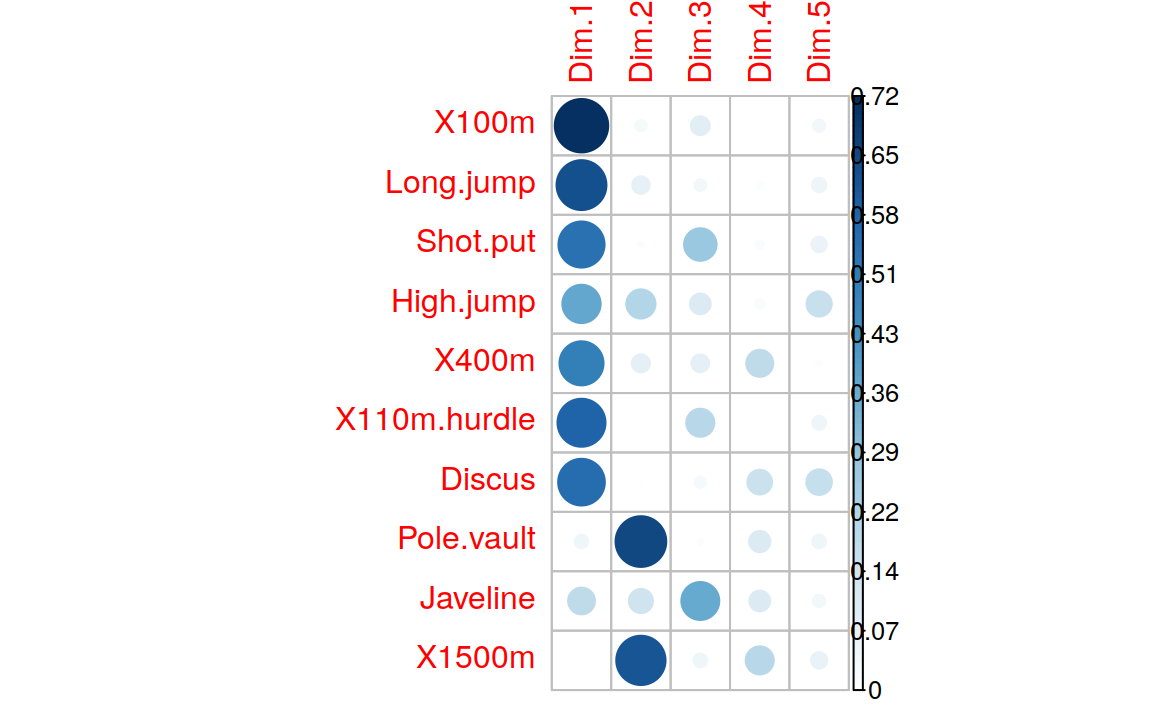
\includegraphics[width=0.7\linewidth]{meta_133-variable_importance_files/figure-latex/unnamed-chunk-15-1} \end{center}

\hypertarget{conclusion}{%
\section{Conclusion}\label{conclusion}}

Hope you find these methods useful. As it turns out different methods showed different variables as important, or at least the degree of importance changed. This need not be a conflict, because each method gives a different perspective of how the variable can be useful depending on how the algorithms learn \texttt{Y\ \textasciitilde{}\ x}. So its cool.

If you find any code breaks or bugs, report the issue here or just write it below.

\hypertarget{imputting-missing-values-with-random-forest}{%
\chapter{Imputting missing values with Random Forest}\label{imputting-missing-values-with-random-forest}}

\hypertarget{flu-prediction.-fluh7n9_china_2013-dataset}{%
\section{\texorpdfstring{Flu Prediction. \texttt{fluH7N9\_china\_2013} dataset}{Flu Prediction. fluH7N9\_china\_2013 dataset}}\label{flu-prediction.-fluh7n9_china_2013-dataset}}

Source: \url{https://shirinsplayground.netlify.com/2018/04/flu_prediction/}

\begin{Shaded}
\begin{Highlighting}[]
\KeywordTok{library}\NormalTok{(outbreaks)}
\KeywordTok{library}\NormalTok{(tidyverse)}
\KeywordTok{library}\NormalTok{(plyr)}
\KeywordTok{library}\NormalTok{(mice)}
\KeywordTok{library}\NormalTok{(caret)}
\KeywordTok{library}\NormalTok{(purrr)}
\KeywordTok{library}\NormalTok{(}\StringTok{"tibble"}\NormalTok{)}
\KeywordTok{library}\NormalTok{(}\StringTok{"dplyr"}\NormalTok{)}
\KeywordTok{library}\NormalTok{(}\StringTok{"tidyr"}\NormalTok{)}
\end{Highlighting}
\end{Shaded}

Since I migrated my blog from Github Pages to blogdown and Netlify, I wanted to start migrating (most of) my old posts too - and use that opportunity to update them and make sure the code still works.

Here I am updating my very first machine learning post from 27 Nov 2016: Can we predict flu deaths with Machine Learning and R?. Changes are marked as bold comments.

The main changes I made are:

\begin{itemize}
\item
  using the tidyverse more consistently throughout the analysis
\item
  focusing on comparing multiple imputations from the mice package, rather than comparing different algorithms
\item
  using purrr, map(), nest() and unnest() to model and predict the machine learning algorithm over the different imputed datasets
\end{itemize}

\begin{center}\rule{0.5\linewidth}{\linethickness}\end{center}

Among the many nice R packages containing data collections is the \texttt{outbreaks} package. It contains a dataset on epidemics and among them is data from the 2013 outbreak of influenza A H7N9 in China as analysed by Kucharski et al. (2014):

\begin{quote}
A. Kucharski, H. Mills, A. Pinsent, C. Fraser, M. Van Kerkhove, C. A. Donnelly, and S. Riley. 2014. Distinguishing between reservoir exposure and human-to-human transmission for emerging pathogens using case onset data. PLOS Currents Outbreaks. Mar 7, edition 1. doi: 10.1371/currents.outbreaks.e1473d9bfc99d080ca242139a06c455f.
\end{quote}

\begin{quote}
A. Kucharski, H. Mills, A. Pinsent, C. Fraser, M. Van Kerkhove, C. A. Donnelly, and S. Riley. 2014. Data from: Distinguishing between reservoir exposure and human-to-human transmission for emerging pathogens using case onset data. Dryad Digital Repository. \url{http://dx.doi.org/10.5061/dryad.2g43n}.
\end{quote}

I will be using their data as an example to show how to use Machine Learning algorithms for predicting disease outcome.

\hypertarget{the-data}{%
\section{The data}\label{the-data}}

The dataset contains case ID, date of onset, date of hospitalization, date of outcome, gender, age, province and of course outcome: Death or Recovery.

\hypertarget{pre-processing}{%
\subsection{Pre-processing}\label{pre-processing}}

Change: variable names (i.e.~column names) have been renamed, dots have been replaced with underscores, letters are all lower case now.

Change: I am using the tidyverse notation more consistently.

First, I'm doing some preprocessing, including:

\begin{itemize}
\tightlist
\item
  renaming missing data as NA
\item
  adding an ID column
\item
  setting column types
\item
  gathering date columns
\item
  changing factor names of dates (to make them look nicer in plots) and of province (to combine provinces with few cases)
\end{itemize}

\begin{Shaded}
\begin{Highlighting}[]
\NormalTok{from1 <-}\StringTok{ }\KeywordTok{c}\NormalTok{(}\StringTok{"date_of_onset"}\NormalTok{, }\StringTok{"date_of_hospitalisation"}\NormalTok{, }\StringTok{"date_of_outcome"}\NormalTok{)}
\NormalTok{to1   <-}\StringTok{ }\KeywordTok{c}\NormalTok{(}\StringTok{"date of onset"}\NormalTok{, }\StringTok{"date of hospitalisation"}\NormalTok{, }\StringTok{"date of outcome"}\NormalTok{)}
\NormalTok{from2 <-}\StringTok{ }\KeywordTok{c}\NormalTok{(}\StringTok{"Anhui"}\NormalTok{, }\StringTok{"Beijing"}\NormalTok{, }\StringTok{"Fujian"}\NormalTok{, }\StringTok{"Guangdong"}\NormalTok{, }\StringTok{"Hebei"}\NormalTok{, }\StringTok{"Henan"}\NormalTok{, }
           \StringTok{"Hunan"}\NormalTok{, }\StringTok{"Jiangxi"}\NormalTok{, }\StringTok{"Shandong"}\NormalTok{, }\StringTok{"Taiwan"}\NormalTok{)}
\NormalTok{to2   <-}\StringTok{ }\KeywordTok{rep}\NormalTok{(}\StringTok{"Other"}\NormalTok{, }\DecValTok{10}\NormalTok{)}

\NormalTok{fluH7N9_china_}\DecValTok{2013}\OperatorTok{$}\NormalTok{age[}\KeywordTok{which}\NormalTok{(fluH7N9_china_}\DecValTok{2013}\OperatorTok{$}\NormalTok{age }\OperatorTok{==}\StringTok{ "?"}\NormalTok{)] <-}\StringTok{ }\OtherTok{NA}
\NormalTok{fluH7N9_china_}\DecValTok{2013}\NormalTok{_gather <-}\StringTok{ }\NormalTok{fluH7N9_china_}\DecValTok{2013} \OperatorTok
\StringTok{  }\KeywordTok{mutate}\NormalTok{(}\DataTypeTok{case_id =} \KeywordTok{paste}\NormalTok{(}\StringTok{"case"}\NormalTok{, case_id, }\DataTypeTok{sep =} \StringTok{"_"}\NormalTok{),}
         \DataTypeTok{age =} \KeywordTok{as.numeric}\NormalTok{(age)) }\OperatorTok
\StringTok{  }\KeywordTok{gather}\NormalTok{(Group, Date, date_of_onset}\OperatorTok{:}\NormalTok{date_of_outcome) }\OperatorTok
\StringTok{  }\KeywordTok{mutate}\NormalTok{(}\DataTypeTok{Group =} \KeywordTok{as.factor}\NormalTok{(}\KeywordTok{mapvalues}\NormalTok{(Group, }\DataTypeTok{from =}\NormalTok{ from1, }\DataTypeTok{to =}\NormalTok{ to1)),}
         \DataTypeTok{province =} \KeywordTok{mapvalues}\NormalTok{(province, }\DataTypeTok{from =}\NormalTok{ from2, }\DataTypeTok{to =}\NormalTok{ to2))}

\NormalTok{fluH7N9_china_}\DecValTok{2013}\NormalTok{ <-}\StringTok{ }\KeywordTok{as.tibble}\NormalTok{(fluH7N9_china_}\DecValTok{2013}\NormalTok{)}
\CommentTok{#> Warning: `as.tibble()` is deprecated, use `as_tibble()` (but mind the new semantics).}
\CommentTok{#> This warning is displayed once per session.}
\NormalTok{fluH7N9_china_}\DecValTok{2013}\NormalTok{_gather <-}\StringTok{ }\KeywordTok{as.tibble}\NormalTok{(fluH7N9_china_}\DecValTok{2013}\NormalTok{_gather)}
\KeywordTok{print}\NormalTok{(fluH7N9_china_}\DecValTok{2013}\NormalTok{)}
\CommentTok{#> # A tibble: 136 x 8}
\CommentTok{#>   case_id date_of_onset date_of_hospita~ date_of_outcome outcome gender}
\CommentTok{#>   <fct>   <date>        <date>           <date>          <fct>   <fct> }
\CommentTok{#> 1 1       2013-02-19    NA               2013-03-04      Death   m     }
\CommentTok{#> 2 2       2013-02-27    2013-03-03       2013-03-10      Death   m     }
\CommentTok{#> 3 3       2013-03-09    2013-03-19       2013-04-09      Death   f     }
\CommentTok{#> 4 4       2013-03-19    2013-03-27       NA              <NA>    f     }
\CommentTok{#> 5 5       2013-03-19    2013-03-30       2013-05-15      Recover f     }
\CommentTok{#> 6 6       2013-03-21    2013-03-28       2013-04-26      Death   f     }
\CommentTok{#> # ... with 130 more rows, and 2 more variables: age <fct>, province <fct>}
\end{Highlighting}
\end{Shaded}

I'm also adding a third gender level for unknown gender

\begin{Shaded}
\begin{Highlighting}[]
\KeywordTok{levels}\NormalTok{(fluH7N9_china_}\DecValTok{2013}\NormalTok{_gather}\OperatorTok{$}\NormalTok{gender) <-}\StringTok{ }
\StringTok{  }\KeywordTok{c}\NormalTok{(}\KeywordTok{levels}\NormalTok{(fluH7N9_china_}\DecValTok{2013}\NormalTok{_gather}\OperatorTok{$}\NormalTok{gender), }\StringTok{"unknown"}\NormalTok{)}
\NormalTok{fluH7N9_china_}\DecValTok{2013}\NormalTok{_gather}\OperatorTok{$}\NormalTok{gender[}\KeywordTok{is.na}\NormalTok{(fluH7N9_china_}\DecValTok{2013}\NormalTok{_gather}\OperatorTok{$}\NormalTok{gender)] <-}\StringTok{ "unknown"}
\KeywordTok{print}\NormalTok{(fluH7N9_china_}\DecValTok{2013}\NormalTok{_gather)}
\CommentTok{#> # A tibble: 408 x 7}
\CommentTok{#>   case_id outcome gender   age province Group         Date      }
\CommentTok{#>   <chr>   <fct>   <fct>  <dbl> <fct>    <fct>         <date>    }
\CommentTok{#> 1 case_1  Death   m         58 Shanghai date of onset 2013-02-19}
\CommentTok{#> 2 case_2  Death   m          7 Shanghai date of onset 2013-02-27}
\CommentTok{#> 3 case_3  Death   f         11 Other    date of onset 2013-03-09}
\CommentTok{#> 4 case_4  <NA>    f         18 Jiangsu  date of onset 2013-03-19}
\CommentTok{#> 5 case_5  Recover f         20 Jiangsu  date of onset 2013-03-19}
\CommentTok{#> 6 case_6  Death   f          9 Jiangsu  date of onset 2013-03-21}
\CommentTok{#> # ... with 402 more rows}
\end{Highlighting}
\end{Shaded}

For plotting, I am defining a custom ggplot2 theme:

\begin{Shaded}
\begin{Highlighting}[]
\NormalTok{my_theme <-}\StringTok{ }\ControlFlowTok{function}\NormalTok{(}\DataTypeTok{base_size =} \DecValTok{12}\NormalTok{, }\DataTypeTok{base_family =} \StringTok{"sans"}\NormalTok{)\{}
  \KeywordTok{theme_minimal}\NormalTok{(}\DataTypeTok{base_size =}\NormalTok{ base_size, }\DataTypeTok{base_family =}\NormalTok{ base_family) }\OperatorTok{+}
\StringTok{  }\KeywordTok{theme}\NormalTok{(}
    \DataTypeTok{axis.text =} \KeywordTok{element_text}\NormalTok{(}\DataTypeTok{size =} \DecValTok{12}\NormalTok{),}
    \DataTypeTok{axis.text.x =} \KeywordTok{element_text}\NormalTok{(}\DataTypeTok{angle =} \DecValTok{45}\NormalTok{, }\DataTypeTok{vjust =} \FloatTok{0.5}\NormalTok{, }\DataTypeTok{hjust =} \FloatTok{0.5}\NormalTok{),}
    \DataTypeTok{axis.title =} \KeywordTok{element_text}\NormalTok{(}\DataTypeTok{size =} \DecValTok{14}\NormalTok{),}
    \DataTypeTok{panel.grid.major =} \KeywordTok{element_line}\NormalTok{(}\DataTypeTok{color =} \StringTok{"grey"}\NormalTok{),}
    \DataTypeTok{panel.grid.minor =} \KeywordTok{element_blank}\NormalTok{(),}
    \DataTypeTok{panel.background =} \KeywordTok{element_rect}\NormalTok{(}\DataTypeTok{fill =} \StringTok{"aliceblue"}\NormalTok{),}
    \DataTypeTok{strip.background =} \KeywordTok{element_rect}\NormalTok{(}\DataTypeTok{fill =} \StringTok{"lightgrey"}\NormalTok{, }\DataTypeTok{color =} \StringTok{"grey"}\NormalTok{, }\DataTypeTok{size =} \DecValTok{1}\NormalTok{),}
    \DataTypeTok{strip.text =} \KeywordTok{element_text}\NormalTok{(}\DataTypeTok{face =} \StringTok{"bold"}\NormalTok{, }\DataTypeTok{size =} \DecValTok{12}\NormalTok{, }\DataTypeTok{color =} \StringTok{"black"}\NormalTok{),}
    \DataTypeTok{legend.position =} \StringTok{"bottom"}\NormalTok{,}
    \DataTypeTok{legend.justification =} \StringTok{"top"}\NormalTok{, }
    \DataTypeTok{legend.box =} \StringTok{"horizontal"}\NormalTok{,}
    \DataTypeTok{legend.box.background =} \KeywordTok{element_rect}\NormalTok{(}\DataTypeTok{colour =} \StringTok{"grey50"}\NormalTok{),}
    \DataTypeTok{legend.background =} \KeywordTok{element_blank}\NormalTok{(),}
    \DataTypeTok{panel.border =} \KeywordTok{element_rect}\NormalTok{(}\DataTypeTok{color =} \StringTok{"grey"}\NormalTok{, }\DataTypeTok{fill =} \OtherTok{NA}\NormalTok{, }\DataTypeTok{size =} \FloatTok{0.5}\NormalTok{)}
\NormalTok{  )}
\NormalTok{\}}
\end{Highlighting}
\end{Shaded}

And use that theme to visualize the data:

\begin{Shaded}
\begin{Highlighting}[]
\KeywordTok{ggplot}\NormalTok{(}\DataTypeTok{data =}\NormalTok{ fluH7N9_china_}\DecValTok{2013}\NormalTok{_gather, }\KeywordTok{aes}\NormalTok{(}\DataTypeTok{x =}\NormalTok{ Date, }\DataTypeTok{y =}\NormalTok{ age, }\DataTypeTok{fill =}\NormalTok{ outcome)) }\OperatorTok{+}
\StringTok{  }\KeywordTok{stat_density2d}\NormalTok{(}\KeywordTok{aes}\NormalTok{(}\DataTypeTok{alpha =}\NormalTok{ ..level..), }\DataTypeTok{geom =} \StringTok{"polygon"}\NormalTok{) }\OperatorTok{+}
\StringTok{  }\KeywordTok{geom_jitter}\NormalTok{(}\KeywordTok{aes}\NormalTok{(}\DataTypeTok{color =}\NormalTok{ outcome, }\DataTypeTok{shape =}\NormalTok{ gender), }\DataTypeTok{size =} \FloatTok{1.5}\NormalTok{) }\OperatorTok{+}
\StringTok{  }\KeywordTok{geom_rug}\NormalTok{(}\KeywordTok{aes}\NormalTok{(}\DataTypeTok{color =}\NormalTok{ outcome)) }\OperatorTok{+}
\StringTok{  }\KeywordTok{scale_y_continuous}\NormalTok{(}\DataTypeTok{limits =} \KeywordTok{c}\NormalTok{(}\DecValTok{0}\NormalTok{, }\DecValTok{90}\NormalTok{)) }\OperatorTok{+}
\StringTok{  }\KeywordTok{labs}\NormalTok{(}
    \DataTypeTok{fill =} \StringTok{"Outcome"}\NormalTok{,}
    \DataTypeTok{color =} \StringTok{"Outcome"}\NormalTok{,}
    \DataTypeTok{alpha =} \StringTok{"Level"}\NormalTok{,}
    \DataTypeTok{shape =} \StringTok{"Gender"}\NormalTok{,}
    \DataTypeTok{x =} \StringTok{"Date in 2013"}\NormalTok{,}
    \DataTypeTok{y =} \StringTok{"Age"}\NormalTok{,}
    \DataTypeTok{title =} \StringTok{"2013 Influenza A H7N9 cases in China"}\NormalTok{,}
    \DataTypeTok{subtitle =} \StringTok{"Dataset from 'outbreaks' package (Kucharski et al. 2014)"}\NormalTok{,}
    \DataTypeTok{caption =} \StringTok{""}
\NormalTok{  ) }\OperatorTok{+}
\StringTok{  }\KeywordTok{facet_grid}\NormalTok{(Group }\OperatorTok{~}\StringTok{ }\NormalTok{province) }\OperatorTok{+}
\StringTok{  }\KeywordTok{my_theme}\NormalTok{() }\OperatorTok{+}
\StringTok{  }\KeywordTok{scale_shape_manual}\NormalTok{(}\DataTypeTok{values =} \KeywordTok{c}\NormalTok{(}\DecValTok{15}\NormalTok{, }\DecValTok{16}\NormalTok{, }\DecValTok{17}\NormalTok{)) }\OperatorTok{+}
\StringTok{  }\KeywordTok{scale_color_brewer}\NormalTok{(}\DataTypeTok{palette=}\StringTok{"Set1"}\NormalTok{, }\DataTypeTok{na.value =} \StringTok{"grey50"}\NormalTok{) }\OperatorTok{+}
\StringTok{  }\KeywordTok{scale_fill_brewer}\NormalTok{(}\DataTypeTok{palette=}\StringTok{"Set1"}\NormalTok{)}
\CommentTok{#> Warning: Removed 149 rows containing non-finite values (stat_density2d).}
\CommentTok{#> Warning: Removed 149 rows containing missing values (geom_point).}
\end{Highlighting}
\end{Shaded}

\begin{center}\includegraphics[width=0.7\linewidth]{meta_230-missing_flu_prediction_micex5-sglander_files/figure-latex/unnamed-chunk-6-1} \end{center}

\begin{Shaded}
\begin{Highlighting}[]
\KeywordTok{ggplot}\NormalTok{(}\DataTypeTok{data =}\NormalTok{ fluH7N9_china_}\DecValTok{2013}\NormalTok{_gather, }\KeywordTok{aes}\NormalTok{(}\DataTypeTok{x =}\NormalTok{ Date, }\DataTypeTok{y =}\NormalTok{ age, }\DataTypeTok{color =}\NormalTok{ outcome)) }\OperatorTok{+}
\StringTok{  }\KeywordTok{geom_point}\NormalTok{(}\KeywordTok{aes}\NormalTok{(}\DataTypeTok{color =}\NormalTok{ outcome, }\DataTypeTok{shape =}\NormalTok{ gender), }\DataTypeTok{size =} \FloatTok{1.5}\NormalTok{, }\DataTypeTok{alpha =} \FloatTok{0.6}\NormalTok{) }\OperatorTok{+}
\StringTok{  }\KeywordTok{geom_path}\NormalTok{(}\KeywordTok{aes}\NormalTok{(}\DataTypeTok{group =}\NormalTok{ case_id)) }\OperatorTok{+}
\StringTok{  }\KeywordTok{facet_wrap}\NormalTok{( }\OperatorTok{~}\StringTok{ }\NormalTok{province, }\DataTypeTok{ncol =} \DecValTok{2}\NormalTok{) }\OperatorTok{+}
\StringTok{  }\KeywordTok{my_theme}\NormalTok{() }\OperatorTok{+}
\StringTok{  }\KeywordTok{scale_shape_manual}\NormalTok{(}\DataTypeTok{values =} \KeywordTok{c}\NormalTok{(}\DecValTok{15}\NormalTok{, }\DecValTok{16}\NormalTok{, }\DecValTok{17}\NormalTok{)) }\OperatorTok{+}
\StringTok{  }\KeywordTok{scale_color_brewer}\NormalTok{(}\DataTypeTok{palette=}\StringTok{"Set1"}\NormalTok{, }\DataTypeTok{na.value =} \StringTok{"grey50"}\NormalTok{) }\OperatorTok{+}
\StringTok{  }\KeywordTok{scale_fill_brewer}\NormalTok{(}\DataTypeTok{palette=}\StringTok{"Set1"}\NormalTok{) }\OperatorTok{+}
\StringTok{  }\KeywordTok{labs}\NormalTok{(}
    \DataTypeTok{color =} \StringTok{"Outcome"}\NormalTok{,}
    \DataTypeTok{shape =} \StringTok{"Gender"}\NormalTok{,}
    \DataTypeTok{x =} \StringTok{"Date in 2013"}\NormalTok{,}
    \DataTypeTok{y =} \StringTok{"Age"}\NormalTok{,}
    \DataTypeTok{title =} \StringTok{"2013 Influenza A H7N9 cases in China"}\NormalTok{,}
    \DataTypeTok{subtitle =} \StringTok{"Dataset from 'outbreaks' package (Kucharski et al. 2014)"}\NormalTok{,}
    \DataTypeTok{caption =} \StringTok{"}\CharTok{\textbackslash{}n}\StringTok{Time from onset of flu to outcome."}
\NormalTok{  )}
\CommentTok{#> Warning: Removed 149 rows containing missing values (geom_point).}
\CommentTok{#> Warning: Removed 122 rows containing missing values (geom_path).}
\end{Highlighting}
\end{Shaded}

\begin{center}\includegraphics[width=0.7\linewidth]{meta_230-missing_flu_prediction_micex5-sglander_files/figure-latex/unnamed-chunk-7-1} \end{center}

\hypertarget{features}{%
\section{Features}\label{features}}

In machine learning-speak features are what we call the variables used for model training. Using the right features dramatically influences the accuracy and success of your model.

For this example, I am keeping age, but I am also generating new features from the date information and converting gender and province into numerical values.

\begin{Shaded}
\begin{Highlighting}[]
\NormalTok{delta_dates <-}\StringTok{ }\ControlFlowTok{function}\NormalTok{(onset, ref) \{}
\NormalTok{    d2 =}\StringTok{ }\KeywordTok{as.Date}\NormalTok{(}\KeywordTok{as.character}\NormalTok{(onset), }\DataTypeTok{format =} \StringTok{"%Y-%m-%d"}\NormalTok{)}
\NormalTok{    d1 =}\StringTok{ }\KeywordTok{as.Date}\NormalTok{(}\KeywordTok{as.character}\NormalTok{(ref), }\DataTypeTok{format =} \StringTok{"%Y-%m-%d"}\NormalTok{)}
    \KeywordTok{as.numeric}\NormalTok{(}\KeywordTok{as.character}\NormalTok{(}\KeywordTok{gsub}\NormalTok{(}\StringTok{" days"}\NormalTok{, }\StringTok{""}\NormalTok{, d1 }\OperatorTok{-}\StringTok{ }\NormalTok{d2)))}
\NormalTok{\}}
\end{Highlighting}
\end{Shaded}

\begin{Shaded}
\begin{Highlighting}[]
\NormalTok{dataset <-}\StringTok{ }\NormalTok{fluH7N9_china_}\DecValTok{2013} \OperatorTok
\StringTok{  }\KeywordTok{mutate}\NormalTok{(}
      \DataTypeTok{hospital =} \KeywordTok{as.factor}\NormalTok{(}\KeywordTok{ifelse}\NormalTok{(}\KeywordTok{is.na}\NormalTok{(date_of_hospitalisation), }\DecValTok{0}\NormalTok{, }\DecValTok{1}\NormalTok{)), }
      \DataTypeTok{gender_f =} \KeywordTok{as.factor}\NormalTok{(}\KeywordTok{ifelse}\NormalTok{(gender }\OperatorTok{==}\StringTok{ "f"}\NormalTok{, }\DecValTok{1}\NormalTok{, }\DecValTok{0}\NormalTok{)), }
      \DataTypeTok{province_Jiangsu =} \KeywordTok{as.factor}\NormalTok{(}\KeywordTok{ifelse}\NormalTok{(province }\OperatorTok{==}\StringTok{ "Jiangsu"}\NormalTok{, }\DecValTok{1}\NormalTok{, }\DecValTok{0}\NormalTok{)), }
      \DataTypeTok{province_Shanghai =} \KeywordTok{as.factor}\NormalTok{(}\KeywordTok{ifelse}\NormalTok{(province }\OperatorTok{==}\StringTok{ "Shanghai"}\NormalTok{, }\DecValTok{1}\NormalTok{, }\DecValTok{0}\NormalTok{)), }
      \DataTypeTok{province_Zhejiang =} \KeywordTok{as.factor}\NormalTok{(}\KeywordTok{ifelse}\NormalTok{(province }\OperatorTok{==}\StringTok{ "Zhejiang"}\NormalTok{, }\DecValTok{1}\NormalTok{, }\DecValTok{0}\NormalTok{)), }
      \DataTypeTok{province_other =} \KeywordTok{as.factor}\NormalTok{(}\KeywordTok{ifelse}\NormalTok{(province }\OperatorTok{==}\StringTok{ "Zhejiang"} 
                                           \OperatorTok{|}\StringTok{ }\NormalTok{province }\OperatorTok{==}\StringTok{ "Jiangsu"} 
                                           \OperatorTok{|}\StringTok{ }\NormalTok{province }\OperatorTok{==}\StringTok{ "Shanghai"}\NormalTok{, }\DecValTok{0}\NormalTok{, }\DecValTok{1}\NormalTok{)),}
      
      \DataTypeTok{days_onset_to_outcome =} \KeywordTok{delta_dates}\NormalTok{(date_of_onset, date_of_outcome),}
      \DataTypeTok{days_onset_to_hospital =} \KeywordTok{delta_dates}\NormalTok{(date_of_onset, date_of_hospitalisation),}
      \DataTypeTok{age =}\NormalTok{ age,}
      \DataTypeTok{early_onset =} \KeywordTok{as.factor}\NormalTok{(}\KeywordTok{ifelse}\NormalTok{(date_of_onset }\OperatorTok{<}\StringTok{ }
\StringTok{                                     }\KeywordTok{summary}\NormalTok{(date_of_onset)[[}\DecValTok{3}\NormalTok{]], }\DecValTok{1}\NormalTok{, }\DecValTok{0}\NormalTok{)),}
      \DataTypeTok{early_outcome =} \KeywordTok{as.factor}\NormalTok{(}\KeywordTok{ifelse}\NormalTok{(date_of_outcome }\OperatorTok{<}
\StringTok{                                       }\KeywordTok{summary}\NormalTok{(date_of_outcome)[[}\DecValTok{3}\NormalTok{]], }\DecValTok{1}\NormalTok{, }\DecValTok{0}\NormalTok{))}
\NormalTok{    ) }\OperatorTok\StringTok{ }
\StringTok{  }\KeywordTok{subset}\NormalTok{(}\DataTypeTok{select =} \OperatorTok{-}\KeywordTok{c}\NormalTok{(}\DecValTok{2}\OperatorTok{:}\DecValTok{4}\NormalTok{, }\DecValTok{6}\NormalTok{, }\DecValTok{8}\NormalTok{))}

\KeywordTok{rownames}\NormalTok{(dataset) <-}\StringTok{ }\NormalTok{dataset}\OperatorTok{$}\NormalTok{case_id}
\CommentTok{#> Warning: Setting row names on a tibble is deprecated.}
\NormalTok{dataset[, }\DecValTok{-2}\NormalTok{] <-}\StringTok{ }\KeywordTok{as.numeric}\NormalTok{(}\KeywordTok{as.matrix}\NormalTok{(dataset[, }\DecValTok{-2}\NormalTok{]))}
\KeywordTok{print}\NormalTok{(dataset)}
\CommentTok{#> # A tibble: 136 x 13}
\CommentTok{#>   case_id outcome   age hospital gender_f province_Jiangsu province_Shangh~}
\CommentTok{#> *   <dbl> <fct>   <dbl>    <dbl>    <dbl>            <dbl>            <dbl>}
\CommentTok{#> 1       1 Death      87        0        0                0                1}
\CommentTok{#> 2       2 Death      27        1        0                0                1}
\CommentTok{#> 3       3 Death      35        1        1                0                0}
\CommentTok{#> 4       4 <NA>       45        1        1                1                0}
\CommentTok{#> 5       5 Recover    48        1        1                1                0}
\CommentTok{#> 6       6 Death      32        1        1                1                0}
\CommentTok{#> # ... with 130 more rows, and 6 more variables: province_Zhejiang <dbl>,}
\CommentTok{#> #   province_other <dbl>, days_onset_to_outcome <dbl>,}
\CommentTok{#> #   days_onset_to_hospital <dbl>, early_onset <dbl>, early_outcome <dbl>}
\end{Highlighting}
\end{Shaded}

\begin{Shaded}
\begin{Highlighting}[]
\KeywordTok{summary}\NormalTok{(dataset}\OperatorTok{$}\NormalTok{outcome)}
\CommentTok{#>   Death Recover    NA's }
\CommentTok{#>      32      47      57}
\end{Highlighting}
\end{Shaded}

\hypertarget{imputing-missing-values}{%
\section{Imputing missing values}\label{imputing-missing-values}}

I am using the \texttt{mice} package for imputing missing values

Note: Since publishing this blogpost I learned that the idea behind using mice is to compare different imputations to see how stable they are, instead of picking one imputed set as fixed for the remainder of the analysis. Therefore, I changed the focus of this post a little bit: in the old post I compared many different algorithms and their outcome; in this updated version I am only showing the \textbf{Random Forest} algorithm and focus on \textbf{comparing the different imputed datasets}. I am ignoring feature importance and feature plots because nothing changed compared to the old post.

\begin{Shaded}
\begin{Highlighting}[]
\CommentTok{# plot the missing data in a matrix by variables}
\NormalTok{md_pattern <-}\StringTok{ }\KeywordTok{md.pattern}\NormalTok{(dataset, }\DataTypeTok{rotate.names =} \OtherTok{TRUE}\NormalTok{)}
\end{Highlighting}
\end{Shaded}

\begin{center}\includegraphics[width=0.7\linewidth]{meta_230-missing_flu_prediction_micex5-sglander_files/figure-latex/unnamed-chunk-11-1} \end{center}

\begin{Shaded}
\begin{Highlighting}[]
\NormalTok{dataset_impute <-}\StringTok{ }\KeywordTok{mice}\NormalTok{(}\DataTypeTok{data =}\NormalTok{ dataset[, }\DecValTok{-2}\NormalTok{],  }\DataTypeTok{print =} \OtherTok{FALSE}\NormalTok{)}
\CommentTok{#> Warning: Number of logged events: 150}
\end{Highlighting}
\end{Shaded}

\hypertarget{generate-a-dataframe-of-five-imputting-strategies}{%
\subsection{Generate a dataframe of five imputting strategies}\label{generate-a-dataframe-of-five-imputting-strategies}}

\begin{itemize}
\tightlist
\item
  by default, mice() calculates five (m = 5) imputed data sets
\item
  we can combine them all in one output with the complete(``long'') function
\item
  I did not want to impute missing values in the outcome column, so I have to merge it back in with the imputed data
\end{itemize}

\begin{Shaded}
\begin{Highlighting}[]
\CommentTok{# c(1,2): case_id, outcome}
\NormalTok{datasets_complete <-}\StringTok{ }\KeywordTok{right_join}\NormalTok{(dataset[, }\KeywordTok{c}\NormalTok{(}\DecValTok{1}\NormalTok{, }\DecValTok{2}\NormalTok{)], }
                           \KeywordTok{complete}\NormalTok{(dataset_impute, }\StringTok{"long"}\NormalTok{),}
                           \DataTypeTok{by =} \StringTok{"case_id"}\NormalTok{) }\OperatorTok\StringTok{ }
\StringTok{  }\KeywordTok{mutate}\NormalTok{(}\DataTypeTok{.imp =} \KeywordTok{as.factor}\NormalTok{(.imp)) }\OperatorTok\StringTok{   }
\StringTok{  }\KeywordTok{select}\NormalTok{(}\OperatorTok{-}\NormalTok{.id) }\OperatorTok\StringTok{ }
\StringTok{  }\KeywordTok{print}\NormalTok{()}
\CommentTok{#> # A tibble: 680 x 14}
\CommentTok{#>   case_id outcome .imp    age hospital gender_f province_Jiangsu}
\CommentTok{#>     <dbl> <fct>   <fct> <dbl>    <dbl>    <dbl>            <dbl>}
\CommentTok{#> 1       1 Death   1        87        0        0                0}
\CommentTok{#> 2       2 Death   1        27        1        0                0}
\CommentTok{#> 3       3 Death   1        35        1        1                0}
\CommentTok{#> 4       4 <NA>    1        45        1        1                1}
\CommentTok{#> 5       5 Recover 1        48        1        1                1}
\CommentTok{#> 6       6 Death   1        32        1        1                1}
\CommentTok{#> # ... with 674 more rows, and 7 more variables: province_Shanghai <dbl>,}
\CommentTok{#> #   province_Zhejiang <dbl>, province_other <dbl>,}
\CommentTok{#> #   days_onset_to_outcome <dbl>, days_onset_to_hospital <dbl>,}
\CommentTok{#> #   early_onset <dbl>, early_outcome <dbl>}
\end{Highlighting}
\end{Shaded}

Let's compare the distributions of the five different imputed datasets:

\hypertarget{plot-effect-of-imputting-on-features}{%
\subsection{plot effect of imputting on features}\label{plot-effect-of-imputting-on-features}}

\begin{Shaded}
\begin{Highlighting}[]
\NormalTok{datasets_complete }\OperatorTok
\StringTok{  }\KeywordTok{gather}\NormalTok{(x, y, age}\OperatorTok{:}\NormalTok{early_outcome) }\OperatorTok\StringTok{ }
\StringTok{  }\KeywordTok{ggplot}\NormalTok{(}\KeywordTok{aes}\NormalTok{(}\DataTypeTok{x =}\NormalTok{ y, }\DataTypeTok{fill =}\NormalTok{ .imp, }\DataTypeTok{color =}\NormalTok{ .imp)) }\OperatorTok{+}
\StringTok{    }\KeywordTok{geom_density}\NormalTok{(}\DataTypeTok{alpha =} \FloatTok{0.20}\NormalTok{) }\OperatorTok{+}
\StringTok{  }\KeywordTok{facet_wrap}\NormalTok{(}\OperatorTok{~}\StringTok{ }\NormalTok{x, }\DataTypeTok{ncol =} \DecValTok{3}\NormalTok{, }\DataTypeTok{scales =} \StringTok{"free"}\NormalTok{) }\OperatorTok{+}
\StringTok{    }\KeywordTok{scale_fill_brewer}\NormalTok{(}\DataTypeTok{palette=}\StringTok{"Set1"}\NormalTok{, }\DataTypeTok{na.value =} \StringTok{"grey50"}\NormalTok{) }\OperatorTok{+}
\StringTok{    }\KeywordTok{scale_color_brewer}\NormalTok{(}\DataTypeTok{palette=}\StringTok{"Set1"}\NormalTok{, }\DataTypeTok{na.value =} \StringTok{"grey50"}\NormalTok{) }\OperatorTok{+}
\StringTok{    }\KeywordTok{my_theme}\NormalTok{()}
\end{Highlighting}
\end{Shaded}

\begin{center}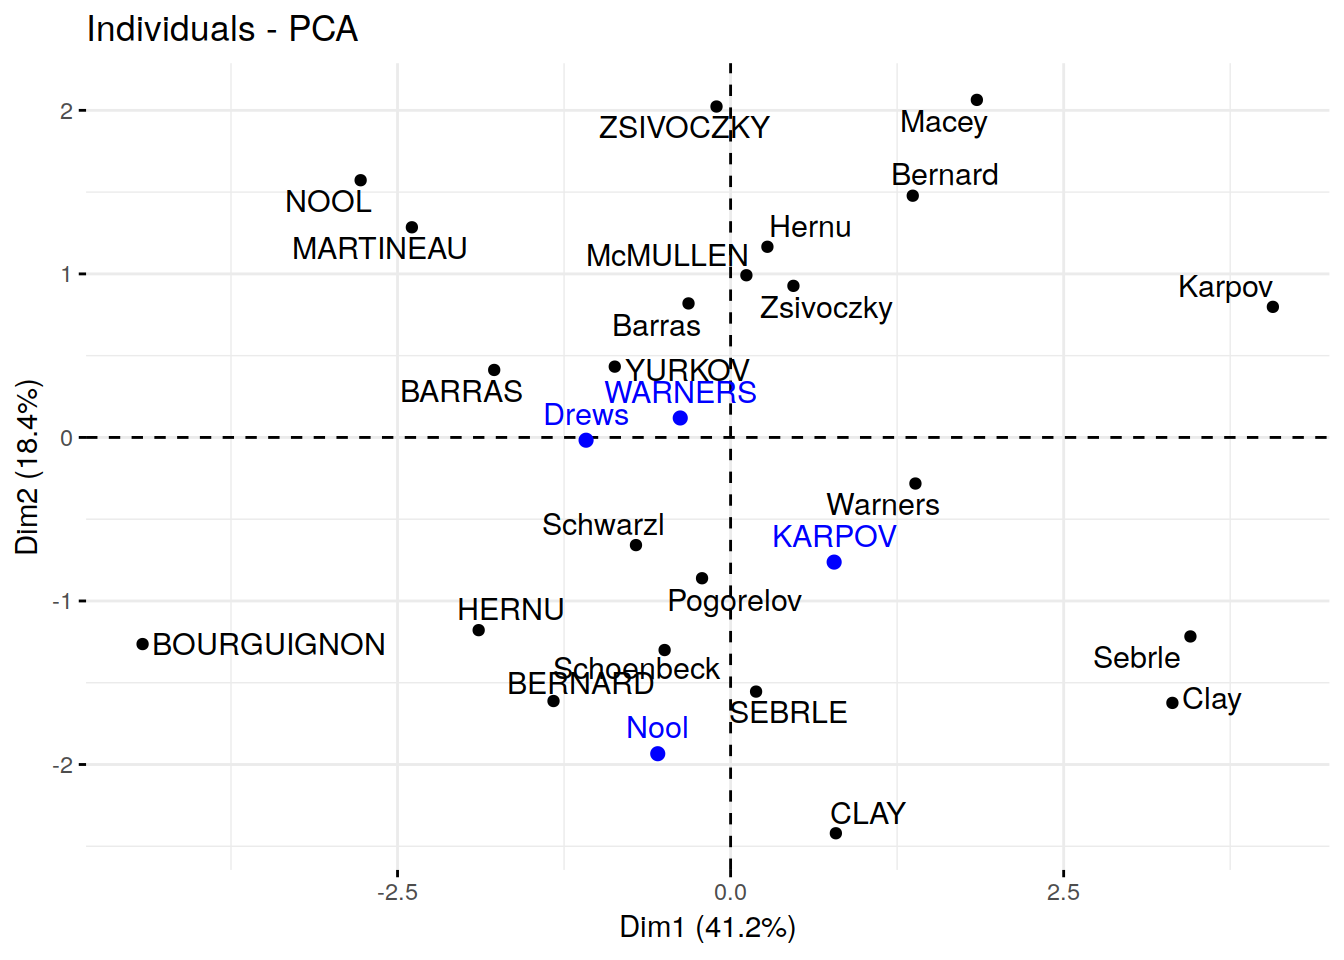
\includegraphics[width=0.7\linewidth]{meta_230-missing_flu_prediction_micex5-sglander_files/figure-latex/unnamed-chunk-14-1} \end{center}

\hypertarget{test-train-and-validation-data-sets}{%
\section{Test, train and validation data sets}\label{test-train-and-validation-data-sets}}

Now, we can go ahead with machine learning!

The dataset contains a few missing values in the outcome column; those will be the test set used for final predictions (see the old blog post for this).

\begin{Shaded}
\begin{Highlighting}[]
\KeywordTok{length}\NormalTok{(}\KeywordTok{which}\NormalTok{(}\KeywordTok{is.na}\NormalTok{(datasets_complete}\OperatorTok{$}\NormalTok{outcome)))}
\KeywordTok{length}\NormalTok{(}\KeywordTok{which}\NormalTok{(}\OperatorTok{!}\KeywordTok{is.na}\NormalTok{(datasets_complete}\OperatorTok{$}\NormalTok{outcome)))}
\CommentTok{#> [1] 285}
\CommentTok{#> [1] 395}
\end{Highlighting}
\end{Shaded}

\begin{Shaded}
\begin{Highlighting}[]
\NormalTok{train_index <-}\StringTok{ }\KeywordTok{which}\NormalTok{(}\KeywordTok{is.na}\NormalTok{(datasets_complete}\OperatorTok{$}\NormalTok{outcome))}
\NormalTok{train_data <-}\StringTok{ }\NormalTok{datasets_complete[}\OperatorTok{-}\NormalTok{train_index, ]}
\NormalTok{test_data  <-}\StringTok{ }\NormalTok{datasets_complete[train_index, }\DecValTok{-2}\NormalTok{]       }\CommentTok{# remove variable outcome}
\end{Highlighting}
\end{Shaded}

\begin{Shaded}
\begin{Highlighting}[]
\KeywordTok{print}\NormalTok{(train_data)}
\CommentTok{#> # A tibble: 395 x 14}
\CommentTok{#>   case_id outcome .imp    age hospital gender_f province_Jiangsu}
\CommentTok{#>     <dbl> <fct>   <fct> <dbl>    <dbl>    <dbl>            <dbl>}
\CommentTok{#> 1       1 Death   1        87        0        0                0}
\CommentTok{#> 2       2 Death   1        27        1        0                0}
\CommentTok{#> 3       3 Death   1        35        1        1                0}
\CommentTok{#> 4       5 Recover 1        48        1        1                1}
\CommentTok{#> 5       6 Death   1        32        1        1                1}
\CommentTok{#> 6       7 Death   1        83        1        0                1}
\CommentTok{#> # ... with 389 more rows, and 7 more variables: province_Shanghai <dbl>,}
\CommentTok{#> #   province_Zhejiang <dbl>, province_other <dbl>,}
\CommentTok{#> #   days_onset_to_outcome <dbl>, days_onset_to_hospital <dbl>,}
\CommentTok{#> #   early_onset <dbl>, early_outcome <dbl>}
\end{Highlighting}
\end{Shaded}

\begin{Shaded}
\begin{Highlighting}[]
\CommentTok{# outcome variable removed}
\KeywordTok{print}\NormalTok{(test_data)}
\CommentTok{#> # A tibble: 285 x 13}
\CommentTok{#>   case_id .imp    age hospital gender_f province_Jiangsu province_Shangh~}
\CommentTok{#>     <dbl> <fct> <dbl>    <dbl>    <dbl>            <dbl>            <dbl>}
\CommentTok{#> 1       4 1        45        1        1                1                0}
\CommentTok{#> 2       9 1        67        1        0                0                0}
\CommentTok{#> 3      15 1        61        0        1                1                0}
\CommentTok{#> 4      16 1        79        0        0                1                0}
\CommentTok{#> 5      22 1        85        1        0                1                0}
\CommentTok{#> 6      28 1        79        0        0                0                0}
\CommentTok{#> # ... with 279 more rows, and 6 more variables: province_Zhejiang <dbl>,}
\CommentTok{#> #   province_other <dbl>, days_onset_to_outcome <dbl>,}
\CommentTok{#> #   days_onset_to_hospital <dbl>, early_onset <dbl>, early_outcome <dbl>}
\end{Highlighting}
\end{Shaded}

The remainder of the data will be used for modeling. Here, I am splitting the data into 70\% training and 30\% test data.

Because I want to model each imputed dataset separately, I am using the \texttt{nest()} and \texttt{map()} functions.

\begin{Shaded}
\begin{Highlighting}[]
\NormalTok{train_data_nest <-}\StringTok{ }\NormalTok{train_data }\OperatorTok
\StringTok{  }\KeywordTok{group_by}\NormalTok{(.imp) }\OperatorTok
\StringTok{  }\KeywordTok{nest}\NormalTok{() }\OperatorTok
\StringTok{  }\KeywordTok{print}\NormalTok{()}
\CommentTok{#> # A tibble: 5 x 2}
\CommentTok{#>   .imp  data              }
\CommentTok{#>   <fct> <list>            }
\CommentTok{#> 1 1     <tibble [79 x 13]>}
\CommentTok{#> 2 2     <tibble [79 x 13]>}
\CommentTok{#> 3 3     <tibble [79 x 13]>}
\CommentTok{#> 4 4     <tibble [79 x 13]>}
\CommentTok{#> 5 5     <tibble [79 x 13]>}
\end{Highlighting}
\end{Shaded}

\begin{Shaded}
\begin{Highlighting}[]
\CommentTok{# split the training data in validation training and validation test}
\KeywordTok{set.seed}\NormalTok{(}\DecValTok{42}\NormalTok{)}
\NormalTok{val_data <-}\StringTok{ }\NormalTok{train_data_nest }\OperatorTok\StringTok{ }
\StringTok{  }\KeywordTok{mutate}\NormalTok{(}\DataTypeTok{val_index =} \KeywordTok{map}\NormalTok{(data, }\OperatorTok{~}\StringTok{ }\KeywordTok{createDataPartition}\NormalTok{(.}\OperatorTok{$}\NormalTok{outcome, }
                                                     \DataTypeTok{p =} \FloatTok{0.7}\NormalTok{, }
                                               \DataTypeTok{list =} \OtherTok{FALSE}\NormalTok{)),}
         \DataTypeTok{val_train_data =} \KeywordTok{map2}\NormalTok{(data, val_index, }\OperatorTok{~}\StringTok{ }\NormalTok{.x[.y, ]),}
         \DataTypeTok{val_test_data  =} \KeywordTok{map2}\NormalTok{(data, val_index, }\OperatorTok{~}\StringTok{ }\NormalTok{.x[}\OperatorTok{-}\NormalTok{.y, ])) }\OperatorTok\StringTok{ }
\StringTok{  }\KeywordTok{print}\NormalTok{()}
\CommentTok{#> # A tibble: 5 x 5}
\CommentTok{#>   .imp  data            val_index        val_train_data    val_test_data   }
\CommentTok{#>   <fct> <list>          <list>           <list>            <list>          }
\CommentTok{#> 1 1     <tibble [79 x ~ <int[,1] [56 x ~ <tibble [56 x 13~ <tibble [23 x 1~}
\CommentTok{#> 2 2     <tibble [79 x ~ <int[,1] [56 x ~ <tibble [56 x 13~ <tibble [23 x 1~}
\CommentTok{#> 3 3     <tibble [79 x ~ <int[,1] [56 x ~ <tibble [56 x 13~ <tibble [23 x 1~}
\CommentTok{#> 4 4     <tibble [79 x ~ <int[,1] [56 x ~ <tibble [56 x 13~ <tibble [23 x 1~}
\CommentTok{#> 5 5     <tibble [79 x ~ <int[,1] [56 x ~ <tibble [56 x 13~ <tibble [23 x 1~}
\end{Highlighting}
\end{Shaded}

\hypertarget{machine-learning-algorithms}{%
\section{Machine Learning algorithms}\label{machine-learning-algorithms}}

\hypertarget{random-forest}{%
\subsection{Random Forest}\label{random-forest}}

To make the code tidier, I am first defining the modeling function with the parameters I want.

\begin{Shaded}
\begin{Highlighting}[]
\NormalTok{model_function <-}\StringTok{ }\ControlFlowTok{function}\NormalTok{(df) \{}
\NormalTok{  caret}\OperatorTok{::}\KeywordTok{train}\NormalTok{(outcome }\OperatorTok{~}\StringTok{ }\NormalTok{.,}
               \DataTypeTok{data =}\NormalTok{ df,}
               \DataTypeTok{method =} \StringTok{"rf"}\NormalTok{,}
               \DataTypeTok{preProcess =} \KeywordTok{c}\NormalTok{(}\StringTok{"scale"}\NormalTok{, }\StringTok{"center"}\NormalTok{),}
               \DataTypeTok{trControl =} \KeywordTok{trainControl}\NormalTok{(}\DataTypeTok{method =} \StringTok{"repeatedcv"}\NormalTok{, }
                                        \DataTypeTok{number =} \DecValTok{5}\NormalTok{, }
                                        \DataTypeTok{repeats =} \DecValTok{3}\NormalTok{, }
                                        \DataTypeTok{verboseIter =} \OtherTok{FALSE}\NormalTok{))}
\NormalTok{\}}
\end{Highlighting}
\end{Shaded}

\hypertarget{add-model-and-prediction-to-nested-dataframe-and-calculate}{%
\subsection{Add model and prediction to nested dataframe and calculate}\label{add-model-and-prediction-to-nested-dataframe-and-calculate}}

Next, I am using the nested tibble from before to map() the model function, predict the outcome and calculate confusion matrices.

\hypertarget{add-model-list-column}{%
\subsubsection{add model list-column}\label{add-model-list-column}}

\begin{Shaded}
\begin{Highlighting}[]
\NormalTok{val_data_model <-}\StringTok{ }\NormalTok{val_data }\OperatorTok
\StringTok{  }\KeywordTok{mutate}\NormalTok{(}\DataTypeTok{model =} \KeywordTok{map}\NormalTok{(val_train_data, }\OperatorTok{~}\StringTok{ }\KeywordTok{model_function}\NormalTok{(.x))) }\OperatorTok\StringTok{ }
\StringTok{  }\KeywordTok{select}\NormalTok{(}\OperatorTok{-}\NormalTok{val_index) }\OperatorTok\StringTok{ }
\StringTok{  }\KeywordTok{print}\NormalTok{()}
\CommentTok{#> # A tibble: 5 x 5}
\CommentTok{#>   .imp  data               val_train_data     val_test_data      model  }
\CommentTok{#>   <fct> <list>             <list>             <list>             <list> }
\CommentTok{#> 1 1     <tibble [79 x 13]> <tibble [56 x 13]> <tibble [23 x 13]> <train>}
\CommentTok{#> 2 2     <tibble [79 x 13]> <tibble [56 x 13]> <tibble [23 x 13]> <train>}
\CommentTok{#> 3 3     <tibble [79 x 13]> <tibble [56 x 13]> <tibble [23 x 13]> <train>}
\CommentTok{#> 4 4     <tibble [79 x 13]> <tibble [56 x 13]> <tibble [23 x 13]> <train>}
\CommentTok{#> 5 5     <tibble [79 x 13]> <tibble [56 x 13]> <tibble [23 x 13]> <train>}
\end{Highlighting}
\end{Shaded}

\hypertarget{add-prediction-and-confusion-matrix-list-columns}{%
\subsubsection{add prediction and confusion matrix list-columns}\label{add-prediction-and-confusion-matrix-list-columns}}

\begin{Shaded}
\begin{Highlighting}[]
\KeywordTok{set.seed}\NormalTok{(}\DecValTok{42}\NormalTok{)}
\NormalTok{val_data_model <-}\StringTok{ }\NormalTok{val_data_model }\OperatorTok
\StringTok{  }\KeywordTok{mutate}\NormalTok{(}
         \DataTypeTok{predict =} \KeywordTok{map2}\NormalTok{(model, val_test_data, }\OperatorTok{~}\StringTok{ }
\StringTok{                            }\KeywordTok{data.frame}\NormalTok{(}\DataTypeTok{prediction =} \KeywordTok{predict}\NormalTok{(.x, .y[, }\DecValTok{-2}\NormalTok{]))),}
         \DataTypeTok{predict_prob =} \KeywordTok{map2}\NormalTok{(model, val_test_data, }\OperatorTok{~}\StringTok{ }
\StringTok{                            }\KeywordTok{data.frame}\NormalTok{(}\DataTypeTok{outcome =}\NormalTok{ .y[, }\DecValTok{2}\NormalTok{], }
                            \DataTypeTok{prediction =} \KeywordTok{predict}\NormalTok{(.x, .y[, }\DecValTok{-2}\NormalTok{], }\DataTypeTok{type =} \StringTok{"prob"}\NormalTok{))),}
         \DataTypeTok{confusion_matrix =} \KeywordTok{map2}\NormalTok{(val_test_data, predict, }\OperatorTok{~}\StringTok{ }
\StringTok{                                     }\KeywordTok{confusionMatrix}\NormalTok{(.x}\OperatorTok{$}\NormalTok{outcome, .y}\OperatorTok{$}\NormalTok{prediction)),}
         \DataTypeTok{confusion_matrix_tbl =} \KeywordTok{map}\NormalTok{(confusion_matrix, }\OperatorTok{~}\StringTok{ }\KeywordTok{as.tibble}\NormalTok{(.x}\OperatorTok{$}\NormalTok{table))) }\OperatorTok\StringTok{ }
\StringTok{  }\KeywordTok{print}\NormalTok{()}
\CommentTok{#> # A tibble: 5 x 9}
\CommentTok{#>   .imp  data  val_train_data val_test_data model predict predict_prob}
\CommentTok{#>   <fct> <lis> <list>         <list>        <lis> <list>  <list>      }
\CommentTok{#> 1 1     <tib~ <tibble [56 x~ <tibble [23 ~ <tra~ <df[,1~ <df[,3] [23~}
\CommentTok{#> 2 2     <tib~ <tibble [56 x~ <tibble [23 ~ <tra~ <df[,1~ <df[,3] [23~}
\CommentTok{#> 3 3     <tib~ <tibble [56 x~ <tibble [23 ~ <tra~ <df[,1~ <df[,3] [23~}
\CommentTok{#> 4 4     <tib~ <tibble [56 x~ <tibble [23 ~ <tra~ <df[,1~ <df[,3] [23~}
\CommentTok{#> 5 5     <tib~ <tibble [56 x~ <tibble [23 ~ <tra~ <df[,1~ <df[,3] [23~}
\CommentTok{#> # ... with 2 more variables: confusion_matrix <list>,}
\CommentTok{#> #   confusion_matrix_tbl <list>}
\end{Highlighting}
\end{Shaded}

\begin{quote}
Finally, we have a nested dataframe of 5 rows or cases, one per imputting strategy with its corresponding models and prediction results.
\end{quote}

\hypertarget{comparing-accuracy-of-models}{%
\section{Comparing accuracy of models}\label{comparing-accuracy-of-models}}

To compare how the different imputations did, I am plotting the confusion matrices:

\begin{Shaded}
\begin{Highlighting}[]
\NormalTok{val_data_model_unnest <-}\StringTok{ }\NormalTok{val_data_model }\OperatorTok
\StringTok{  }\KeywordTok{unnest}\NormalTok{(confusion_matrix_tbl) }\OperatorTok
\StringTok{  }\KeywordTok{print}\NormalTok{()}
\CommentTok{#> # A tibble: 20 x 4}
\CommentTok{#>   .imp  Prediction Reference     n}
\CommentTok{#>   <fct> <chr>      <chr>     <int>}
\CommentTok{#> 1 1     Death      Death         5}
\CommentTok{#> 2 1     Recover    Death         3}
\CommentTok{#> 3 1     Death      Recover       4}
\CommentTok{#> 4 1     Recover    Recover      11}
\CommentTok{#> 5 2     Death      Death         3}
\CommentTok{#> 6 2     Recover    Death         3}
\CommentTok{#> # ... with 14 more rows}
\end{Highlighting}
\end{Shaded}

\begin{Shaded}
\begin{Highlighting}[]
\NormalTok{val_data_model_unnest }\OperatorTok\StringTok{ }
\StringTok{  }\KeywordTok{ggplot}\NormalTok{(}\KeywordTok{aes}\NormalTok{(}\DataTypeTok{x =}\NormalTok{ Prediction, }\DataTypeTok{y =}\NormalTok{ Reference, }\DataTypeTok{fill =}\NormalTok{ n)) }\OperatorTok{+}
\StringTok{    }\KeywordTok{facet_wrap}\NormalTok{(}\OperatorTok{~}\StringTok{ }\NormalTok{.imp, }\DataTypeTok{ncol =} \DecValTok{5}\NormalTok{, }\DataTypeTok{scales =} \StringTok{"free"}\NormalTok{) }\OperatorTok{+}
\StringTok{    }\KeywordTok{geom_tile}\NormalTok{() }\OperatorTok{+}
\StringTok{    }\KeywordTok{my_theme}\NormalTok{()}
\end{Highlighting}
\end{Shaded}

\begin{center}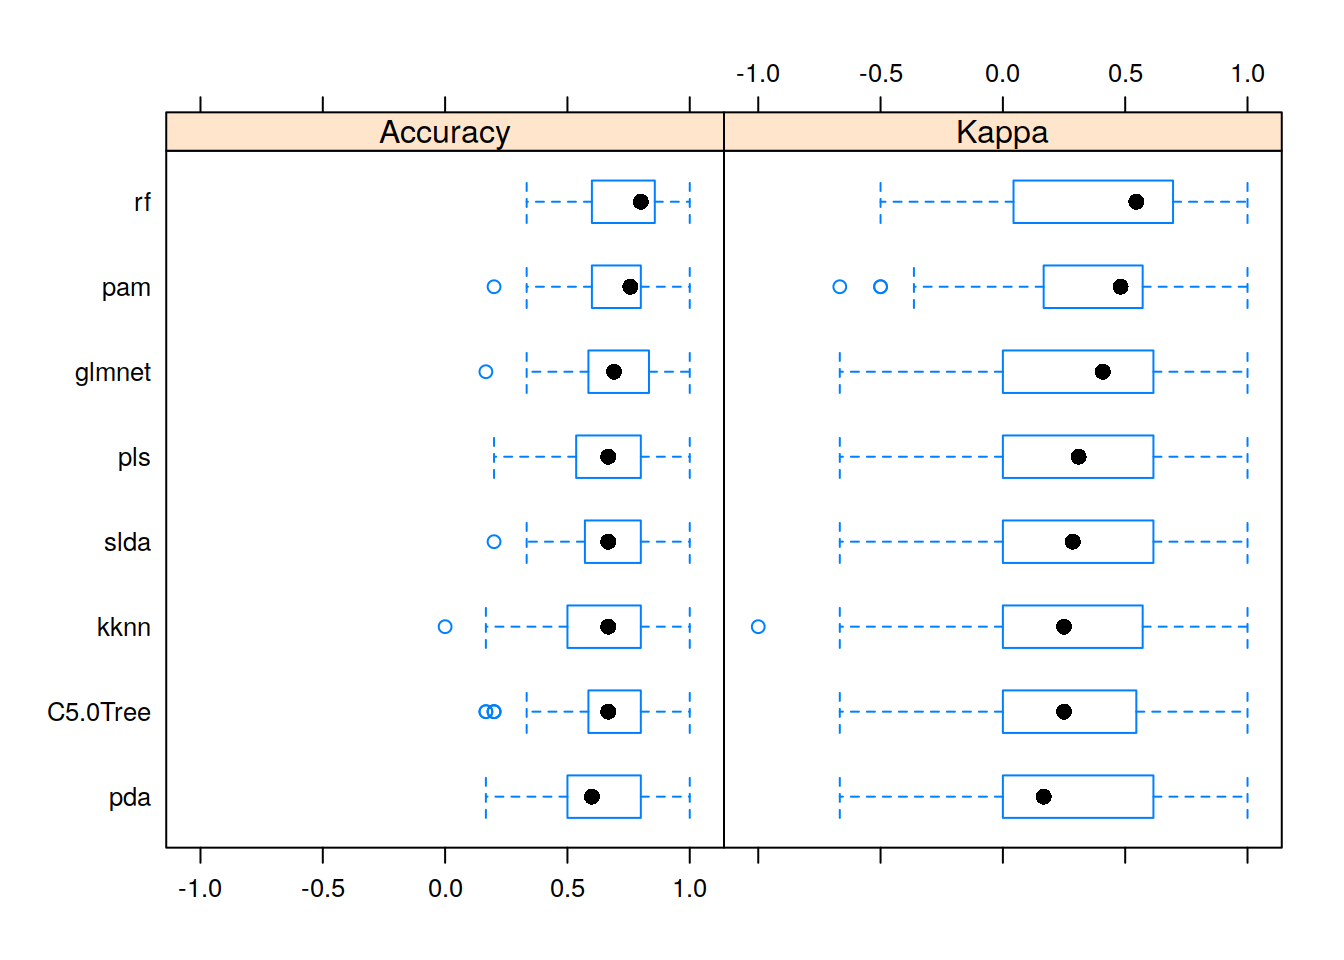
\includegraphics[width=0.7\linewidth]{meta_230-missing_flu_prediction_micex5-sglander_files/figure-latex/unnamed-chunk-25-1} \end{center}

and the prediction probabilities for correct and wrong predictions:

\begin{Shaded}
\begin{Highlighting}[]
\NormalTok{val_data_model_gather <-}\StringTok{ }\NormalTok{val_data_model }\OperatorTok
\StringTok{  }\KeywordTok{unnest}\NormalTok{(predict_prob) }\OperatorTok
\StringTok{  }\KeywordTok{gather}\NormalTok{(x, y, prediction.Death}\OperatorTok{:}\NormalTok{prediction.Recover) }\OperatorTok
\StringTok{  }\KeywordTok{print}\NormalTok{()}
\CommentTok{#> # A tibble: 230 x 4}
\CommentTok{#>   .imp  outcome x                    y}
\CommentTok{#>   <fct> <fct>   <chr>            <dbl>}
\CommentTok{#> 1 1     Death   prediction.Death 0.758}
\CommentTok{#> 2 1     Recover prediction.Death 0.864}
\CommentTok{#> 3 1     Death   prediction.Death 0.828}
\CommentTok{#> 4 1     Death   prediction.Death 0.828}
\CommentTok{#> 5 1     Recover prediction.Death 0.342}
\CommentTok{#> 6 1     Recover prediction.Death 0.552}
\CommentTok{#> # ... with 224 more rows}
\end{Highlighting}
\end{Shaded}

\begin{Shaded}
\begin{Highlighting}[]
\NormalTok{val_data_model_gather }\OperatorTok\StringTok{ }
\StringTok{  }\KeywordTok{ggplot}\NormalTok{(}\KeywordTok{aes}\NormalTok{(}\DataTypeTok{x =}\NormalTok{ x, }\DataTypeTok{y =}\NormalTok{ y, }\DataTypeTok{fill =}\NormalTok{ outcome)) }\OperatorTok{+}
\StringTok{    }\KeywordTok{facet_wrap}\NormalTok{(}\OperatorTok{~}\StringTok{ }\NormalTok{.imp, }\DataTypeTok{ncol =} \DecValTok{5}\NormalTok{) }\OperatorTok{+}
\StringTok{    }\KeywordTok{geom_boxplot}\NormalTok{() }\OperatorTok{+}
\StringTok{    }\KeywordTok{scale_fill_brewer}\NormalTok{(}\DataTypeTok{palette=}\StringTok{"Set1"}\NormalTok{, }\DataTypeTok{na.value =} \StringTok{"grey50"}\NormalTok{) }\OperatorTok{+}
\StringTok{    }\KeywordTok{my_theme}\NormalTok{()}
\end{Highlighting}
\end{Shaded}

\begin{center}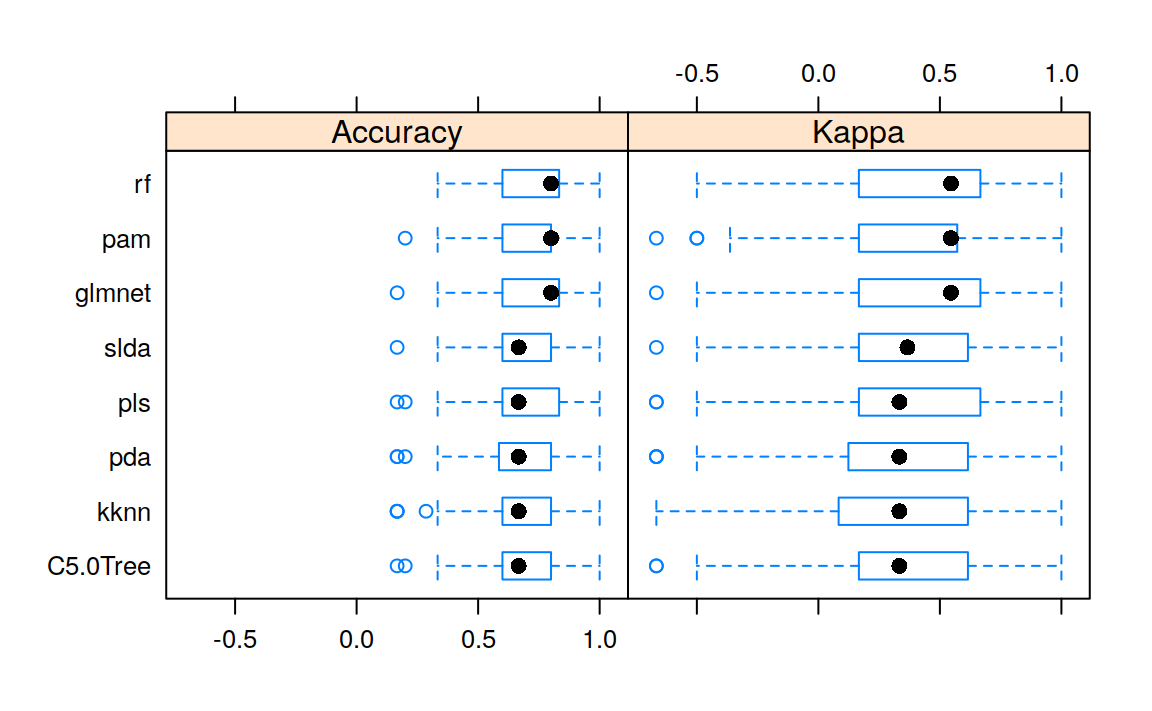
\includegraphics[width=0.7\linewidth]{meta_230-missing_flu_prediction_micex5-sglander_files/figure-latex/unnamed-chunk-27-1} \end{center}

Hope, you found that example interesting and helpful!

\begin{Shaded}
\begin{Highlighting}[]
\KeywordTok{sessionInfo}\NormalTok{()}
\CommentTok{#> R version 3.6.0 (2019-04-26)}
\CommentTok{#> Platform: x86_64-pc-linux-gnu (64-bit)}
\CommentTok{#> Running under: Ubuntu 18.04.3 LTS}
\CommentTok{#> }
\CommentTok{#> Matrix products: default}
\CommentTok{#> BLAS/LAPACK: /usr/lib/x86_64-linux-gnu/libopenblasp-r0.2.20.so}
\CommentTok{#> }
\CommentTok{#> locale:}
\CommentTok{#>  [1] LC_CTYPE=en_US.UTF-8       LC_NUMERIC=C              }
\CommentTok{#>  [3] LC_TIME=en_US.UTF-8        LC_COLLATE=en_US.UTF-8    }
\CommentTok{#>  [5] LC_MONETARY=en_US.UTF-8    LC_MESSAGES=en_US.UTF-8   }
\CommentTok{#>  [7] LC_PAPER=en_US.UTF-8       LC_NAME=C                 }
\CommentTok{#>  [9] LC_ADDRESS=C               LC_TELEPHONE=C            }
\CommentTok{#> [11] LC_MEASUREMENT=en_US.UTF-8 LC_IDENTIFICATION=C       }
\CommentTok{#> }
\CommentTok{#> attached base packages:}
\CommentTok{#> [1] stats     graphics  grDevices utils     datasets  methods   base     }
\CommentTok{#> }
\CommentTok{#> other attached packages:}
\CommentTok{#>  [1] caret_6.0-84    mice_3.4.0      lattice_0.20-38 plyr_1.8.4     }
\CommentTok{#>  [5] forcats_0.4.0   stringr_1.4.0   dplyr_0.8.0.1   purrr_0.3.2    }
\CommentTok{#>  [9] readr_1.3.1     tidyr_0.8.3     tibble_2.1.1    ggplot2_3.1.1  }
\CommentTok{#> [13] tidyverse_1.2.1 outbreaks_1.5.0 logging_0.9-107}
\CommentTok{#> }
\CommentTok{#> loaded via a namespace (and not attached):}
\CommentTok{#>  [1] nlme_3.1-139        lubridate_1.7.4     RColorBrewer_1.1-2 }
\CommentTok{#>  [4] httr_1.4.0          rprojroot_1.3-2     tools_3.6.0        }
\CommentTok{#>  [7] backports_1.1.4     utf8_1.1.4          R6_2.4.0           }
\CommentTok{#> [10] rpart_4.1-15        lazyeval_0.2.2      colorspace_1.4-1   }
\CommentTok{#> [13] jomo_2.6-7          nnet_7.3-12         withr_2.1.2        }
\CommentTok{#> [16] tidyselect_0.2.5    compiler_3.6.0      cli_1.1.0          }
\CommentTok{#> [19] rvest_0.3.3         xml2_1.2.0          labeling_0.3       }
\CommentTok{#> [22] bookdown_0.10       scales_1.0.0        randomForest_4.6-14}
\CommentTok{#> [25] digest_0.6.18       minqa_1.2.4         rmarkdown_1.12     }
\CommentTok{#> [28] pkgconfig_2.0.2     htmltools_0.3.6     lme4_1.1-21        }
\CommentTok{#> [31] rlang_0.3.4         readxl_1.3.1        rstudioapi_0.10    }
\CommentTok{#> [34] generics_0.0.2      jsonlite_1.6        ModelMetrics_1.2.2 }
\CommentTok{#> [37] magrittr_1.5        Matrix_1.2-17       Rcpp_1.0.1         }
\CommentTok{#> [40] munsell_0.5.0       fansi_0.4.0         stringi_1.4.3      }
\CommentTok{#> [43] yaml_2.2.0          MASS_7.3-51.4       recipes_0.1.5      }
\CommentTok{#> [46] grid_3.6.0          parallel_3.6.0      mitml_0.3-7        }
\CommentTok{#> [49] crayon_1.3.4        haven_2.1.0         splines_3.6.0      }
\CommentTok{#> [52] hms_0.4.2           zeallot_0.1.0       knitr_1.22         }
\CommentTok{#> [55] pillar_1.4.0        boot_1.3-22         reshape2_1.4.3     }
\CommentTok{#> [58] codetools_0.2-16    stats4_3.6.0        pan_1.6            }
\CommentTok{#> [61] glue_1.3.1          evaluate_0.13       data.table_1.12.2  }
\CommentTok{#> [64] modelr_0.1.4        vctrs_0.1.0         nloptr_1.2.1       }
\CommentTok{#> [67] foreach_1.4.4       cellranger_1.1.0    gtable_0.3.0       }
\CommentTok{#> [70] assertthat_0.2.1    xfun_0.6            gower_0.2.0        }
\CommentTok{#> [73] prodlim_2018.04.18  broom_0.5.2         e1071_1.7-1        }
\CommentTok{#> [76] class_7.3-15        survival_2.44-1.1   timeDate_3043.102  }
\CommentTok{#> [79] iterators_1.0.10    lava_1.6.5          ipred_0.9-9}
\end{Highlighting}
\end{Shaded}

\bibliography{book.bib,packages.bib}


\end{document}
